\chapter{Methodology}

Building on the theoretical foundations of Bayesian inference and variational methods, this chapter develops the methodological framework of the thesis. We formalize the Linear Regression Model (LRM), the Hierarchical Linear Regression Model (HLRM), and the Clustering HLRM (CHLRM), specifying their priors and posterior structures. These models provide the ground on which we implement and compare MCMC, Variational Inference (VI), and Stochastic Variational Inference (SVI), thus establishing the link between theory and application that guides the subsequent empirical analysis.

\section{Model Checking and Goodness-of-Fit}

We evaluate the adequacy of Bayesian modeling by combining posterior predictive checks with information criteria that balance fit and complexity. Posterior predictive checks focus on absolute model adequacy, while criteria such as the Deviance Information Criterion (DIC) and the Watanabe–Akaike Information Criterion (WAIC) address relative model comparison.

\vspace{0.5cm}

To begin, we use posterior predictive $p$-values (ppp-values), which are obtained by comparing replicated data from the posterior predictive distribution with the observed data (see  \cite{GELMAN14}). For a chosen discrepancy statistic $t(\cdot)$, the posterior predictive $p$-value is defined as

\begin{equation}
p_{pp} = p\left(t(\bm{\tilde{y}}) > t(\bm y)\mid \bm y,\hat{\bm\Theta}\right),
\end{equation}

where $\bm{\tilde{y}} \stackrel{\text{iid}}{\sim} p(y \mid\hat{\bm\Theta})$ denotes a replicated dataset. Values of $p_{pp}$ close to $0.5$ indicate that the model reproduces relevant features of the data, whereas values near $0$ or $1$ suggest a potential lack of fit. Although ppp-values are known to be conservative, they remain a flexible and widely used diagnostic in hierarchical modeling (\cite{SOSA}).

\vspace{0.5cm}

As a complement, we consider predictive performance criteria that penalize complexity. The Deviance Information Criterion (DIC) is defined as
\begin{equation}
\label{DIC}
\text{DIC} = -2\log p(\bm{y}\mid \hat{\bm{\Theta}}) + 2p_{\text{DIC}},
\end{equation}
where $\hat{\bm{\Theta}}$ is the posterior mean of the parameters and $p_{\text{DIC}}$ is the effective number of parameters, computed either as

$$
p_{\text{DIC}} = 2\log p(\bm{y}\mid \hat{\bm{\Theta}}) - 2\mathbb{E}\left[\log p(\bm{y}\mid \bm{\Theta}) \mid \bm{y}\right]
$$

or equivalently as the posterior variance of the log-likelihood. DIC has been widely applied in hierarchical regression contexts (\cite{HOFF}), but it may perform poorly when posterior distributions are multimodal or weakly identifiable.

\vspace{0.5cm}

A more robust alternative is the Watanabe–Akaike Information Criterion (WAIC), which is fully Bayesian and based on pointwise predictive density contributions (\cite{watanabe}). It is defined as

\begin{equation}
\label{WAIC}
\text{WAIC} = -2\sum_{i=1}^n \log \mathsf{E}\left[p(y_i\mid \bm{\Theta}) \mid \bm{y}\right] + 2p_{\text{WAIC}},
\end{equation}
with
$$
p_{\text{WAIC}} = \sum_{i=1}^n \mathsf{Var}\left(\log p(y_i\mid \bm{\Theta}) \mid \mathbf{y}\right).
$$

WAIC can be viewed as a Bayesian approximation to cross-validation and is typically more stable than DIC in complex hierarchical or nonparametric models (\cite{SOSA}).

\vspace{0.5cm}

In summary, posterior predictive $p$-values provide evidence of absolute model adequacy, while DIC and WAIC are relative criteria. Among these, WAIC is generally preferred for hierarchical models due to its theoretical grounding and robustness, although in practice it is advisable to combine all three measures to obtain a comprehensive assessment of model fit and predictive ability.


\section{Normal Linear Regression Model}

In \cite{ML_MURPHY} it states the classical linear regression model like the \textit{work horse} of statistics and supervised machine learning , so as to this model tries to explain variations in  continuous response variable $\bm{y}$ from one or more predictor variables $\bm{x}=(x_{1},\cdots,x_{p})^\top$ , specifying the mean of the response variable as a linear combination of the predictor variables \cite{Christensen2010-ps} , we start the bayesian study of above model as follows:

\begin{equation}
    \label{LRM_i}
    y_i \mid \bm{x}_i,\bm{\beta},\sigma^2\stackrel{\mathsf{iid}}{\sim} \mathsf{N}\left(\bm{x}_i^\top\bm{\beta},\sigma^2\right)\quad\text{for}\quad i=1,\cdots,n
\end{equation}

with $\bm{x}_i=(x_{i1},\cdots,x_{ip})^\top$, which expressed in matricial form is given by:

\begin{equation}
    \label{LRM}
    \bm{y} \mid \bm{X},\bm{\beta},\sigma^2\sim\mathsf{N_n}\left(\bm{X}\bm{\beta},\sigma^2\bm{I_n}\right)
\end{equation}

with $\bm{y}=(y_1,\cdots,y_n)^\top$ the response vector, $\bm{X}=\left[\bm{x}_1,\cdots,\bm{x}_n\right]^\top$ the design matrix , $\bm{\beta}=\left[\beta_1,\cdots,\beta_p\right]^\top$ the vector of parameters and $\sigma^2$ the response variance.

\subsection{Prior Distributions}

To address with a Bayesian approach we define the parameters vector as $\bm{\Theta}=(\bm{\beta},\sigma^2)$ and its priors distributions as follows:

\begin{equation}
    \label{hyper_LRM_1}
    \bm{\beta} \sim \mathsf{N_p}(\bm{\beta}_0, \bm{\Sigma}_0) \quad \text { and } \quad \sigma^2 \sim \mathsf{IG}\left(\nu_0/ 2, \nu_0 \sigma_0^2 / 2\right)
\end{equation}

with $\bm{\beta}_0,\bm{\Sigma}_0,\nu_0,\sigma^2_0$ the hyperparameters of model.


\begin{figure}[H]
    \centering
    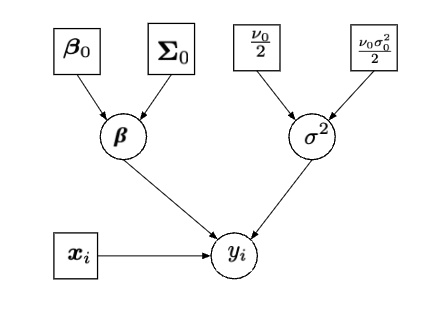
\includegraphics[scale=0.6]{Kap2/DAG_LRM.png}
    \caption{DAG Representation LRM}
    \label{fig:DAG_LRM}
\end{figure}

\subsubsection{Prior elicitation}

Prior elicitation plays a fundamental role in hierarchical linear regression, as it determines how much external information is incorporated into the posterior inference. According to \cite{SOSA}, two main strategies are commonly adopted depending on the availability of prior knowledge. When little or no external evidence is available, it is advisable to use weakly informative priors that contribute minimal influence, such as the \emph{unit information prior} of \cite{KassWasserman1995}. This choice encodes the information equivalent to a single observation and ensures that the prior does not dominate the likelihood, while still guaranteeing mathematical regularity for the posterior, \cite{HOFF} emphasizes that in regression settings, it is often convenient to center the prior mean at the ordinary least squares estimator, setting
\begin{equation}
    \bm{\beta}_0 = \hat{\bm{\beta}}_{\text{OLS}}, \qquad
    \bm{\Sigma}_0 = g \, \sigma^2 \left(\bm{X}^\top \bm{X}\right)^{-1},
\end{equation}
so that the prior on $\bm{\beta}$ represents the information of approximately one data point. Similarly, for the error variance we may use
\begin{equation}
    \nu_0 = 1, \qquad \sigma_0^2 = \hat{\sigma}^2_{\text{OLS}}.
\end{equation}
An alternative is to adopt a scale–invariant prior by setting
\begin{equation}
    \bm{\beta}_0 = \bm{0}, \qquad \bm{\Sigma}_0 = g \, \sigma^2 \left(\bm{X}^\top \bm{X}\right)^{-1},
\end{equation}
with $g=n$, leading to Zellner’s $g$‑prior \cite{Zellner1986}. Both approaches allow the researcher to encode weak or moderate prior information in a way that is consistent with model structure while remaining computationally tractable.


\subsection{Posterior Inference}

\subsubsection{Gibbs Sampling}

For this algorithm, the full conditional distributions (f.c.d.'s) of each parameter in the model $\bm{\Theta} = (\bm{\beta}, \sigma^2)$ are provided, where $p(\cdot \mid \textit{rest})$ denotes the full conditional distribution of each parameter given the remaining parameters, from the full posterior distribution as follows:

\begin{equation}
    \label{POST_LRM}
    \begin{split}
    p(\bm{\Theta} \mid \bm{y}, \bm{X}) 
    &\propto 
p(\bm{y} \mid \bm{X}, \bm{\beta}, \sigma^2) \,
p(\bm{\beta} ) \,
p(\sigma^2 )\\
&\propto\mathsf{N_n}\left(\bm{y}\mid\bm{X}\bm{\beta},\sigma^2\bm{I_n}\right)\times\mathsf{N_p}(\bm{\beta}\mid\bm{\beta}_0, \bm{\Sigma}_0)\times\mathsf{IG}\left(\sigma^2\mid\nu_0/ 2, \nu_0 \sigma_0^2 / 2\right)\\
&\propto (\sigma^2)^{-n/2} 
\exp\left\{ -\frac{1}{2\sigma^2}  (\bm{y} - \bm{X} \bm{\beta})^{\top}
(\bm{y} - \bm{X} \bm{\beta}) \right\} \\
&\quad \times \exp\left\{ -\frac{1}{2} (\bm{\beta} - \bm{\beta}_0)^{\top}
\bm{\Sigma}_0^{-1} (\bm{\beta} - \bm{\beta}_0) \right\} \\
&\quad \times (\sigma^2)^{-(\nu_0/2 + 1)} 
\exp\left\{ -\frac{\nu_0 \sigma_0^2}{2\sigma^2} \right\}
\end{split}
\end{equation}

so, the f.c.d.s are given by:

\begin{itemize}

\item f.c.d of $\bm{\beta}$

\begin{equation}
    \label{LRM_MCMC_Beta}
    \bm{\beta} \mid \text{rest} \sim \mathsf{N_p}\left(\left( \frac{1}{\sigma^2} \bm{X}^\top \bm{X} + \bm{\Sigma}_0^{-1} \right)^{-1}\left( \frac{1}{\sigma^2} \bm{X}^\top \bm{y} + \bm{\Sigma}_0^{-1} \bm{\beta}_0 \right), \left( \frac{1}{\sigma^2} \bm{X}^\top \bm{X} + \bm{\Sigma}_0^{-1} \right)^{-1}\right)
\end{equation}

\item  f.c.d of $\sigma^2$

\begin{equation}
    \label{LRM_MCMC_sigma2}
    \sigma^2 \mid \text{rest} \sim \mathsf{IG}\left( \frac{n + \nu_0}{2}, \frac{\nu_0 \sigma_0^2 + (\bm{y} - \bm{X} \bm{\beta})^\top (\bm{y} - \bm{X} \bm{\beta})}{2} \right)
\end{equation}

\end{itemize}

\begin{algorithm}[H]
\caption{Gibbs Sampling for LRM}
\begin{algorithmic}
\State \textbf{Input} Init values $\bm{\beta}^{(0)}, (\sigma^2)^{(0)}$, hyperparameters: $\bm{\beta}_0,\bm{\Sigma},\nu_0,\sigma_0^2$, data values $\bm{y},\bm{X}$
\For{$b = 1, \dots, B$}
    \State Sample $\bm{\beta}^{(b)} \sim p\left(\bm{\beta} \mid (\sigma^2)^{(b-1)},\bm{y},\bm{X}\right)$ from eq. \ref{LRM_MCMC_Beta}
    \State Sample $(\sigma^2)^{(b)} \sim p\left(\sigma^{2} \mid \bm{\beta}^{(b)},\bm{y},\bm{X}\right)$ from eq. \ref{LRM_MCMC_sigma2}
\EndFor
\State \textbf{Output} Draws $\{\bm{\beta}^{(b)}, (\sigma^2)^{(b)}\}_{b=1}^{B}$ 
\end{algorithmic}
\end{algorithm}

For detailed and explicit derivations, see Appendix \ref{Appendix_B}.


\subsubsection{CAVI}

For this algorithm, the coordinate ascent variational inference updates are presented for each parameter in the model $\bm{\Theta} = (\bm{\beta}, \sigma^2)$. Here, the updates are derived under a mean–field factorization, and each variational factor is optimized while holding the others fixed, as follows:

\begin{equation}
\label{Q_LRM}
q\left(\bm{\Theta}\right)=q(\bm{\beta})q(\sigma^2)
\end{equation}
    

\begin{itemize}

\item Factor $q(\bm{\beta}) = \mathsf{N_p}\left(\bm{\mu}_{\bm{\beta}},\bm{\Sigma}_{\bm{\beta}}\right)$, whit

\begin{equation}
\label{LRM_CAVI_Mu_Beta}
\bm{\mu}_{\bm{\beta}}=\left(\mathsf{E}_{\sigma^2}\left[ \frac{1}{\sigma^2} \right]\bm{X}^\top \bm{X} + \bm{\Sigma}_0^{-1} \right)^{-1}\left(\mathsf{E}_{\sigma^2}\left[ \frac{1}{\sigma^2}\right] \bm{X}^\top \bm{y} + \bm{\Sigma}_0^{-1} \bm{\beta}_0 \right),
\end{equation}

\begin{equation}
\label{LRM_CAVI_sigma2_Beta}
\bm{\Sigma}_{\bm{\beta}} = \left(\mathsf{E}_{\sigma^2}\left[ \frac{1}{\sigma^2} \right]\bm{X}^\top \bm{X} + \bm{\Sigma}_0^{-1} \right)^{-1}
\end{equation}

\item Factor $q(\sigma^2) = \mathsf{IG}\left( a, b \right)$, whit

\begin{equation}
\label{LRM_CAVI_a_sigma2}
a = \frac{n + \nu_0}{2},
\end{equation}

\begin{equation}
\label{LRM_CAVI_b_sigma2}
b = \frac{\nu_0 \sigma_0^2 + \mathsf{E}_{\bm{\beta}}\left[(\bm{y} - \bm{X} \bm{\beta})^{\top}
(\bm{y} - \bm{X} \bm{\beta})  \right]}{2}
\end{equation}

\item ELBO $\mathcal{L}(q(\bm{\Theta}))$

\begin{equation}
\label{LRM_CAVI_ELBO}
\begin{split}
\mathcal{L}(q(\bm{\Theta}))
&=\mathsf{E}_{\bm{\Theta}}\left[\log p(\bm{\Theta},\bm{y}, \bm{X})\right]-\mathsf{E}_{\bm{\Theta}}\left[\log q(\bm{\Theta})\right]\\
&=\mathsf{E}_{\bm{\Theta}}\left[\log p(\bm{y} \mid \bm{X}, \bm{\beta}, \sigma^2)\right] + \left(\mathsf{E}_{\bm{\Theta}}\left[\log  p(\bm{\beta})\right] -\mathsf{E}_{\bm{\beta}}\left[\log q(\bm{\beta})\right]\right)+
\left(\mathsf{E}_{\bm{\Theta}}\left[\log p(\sigma^2 )\right]-\mathsf{E}_{\sigma^2}\left[\log q(\sigma^2)\right]\right)
\end{split}
\end{equation}

\newpage

where:

\begin{itemize}
    \item $\mathsf{E}_{\bm{\Theta}}\left[\log p(\bm{y} \mid \bm{X}, \bm{\beta}, \sigma^2)\right]=-\frac{n}{2}\log(2\pi) - \frac{n}{2}\left(\log b -\psi(a)\right)
- \frac{1}{2}\left(\frac{a}{b}\right)\left((\bm{y} - \bm{X}  \bm\mu_{\bm{\beta}})^{\top}
(\bm{y} - \bm{X} \bm\mu_{\bm{\beta}}) + \operatorname{tr}\left(\bm{X}^{\top}\bm{X}\bm{\Sigma}_{\bm{\beta}}\right)\right)$
\item  $\mathsf{E}_{\bm{\Theta}}\left[\log  p(\bm{\beta})\right]=- \frac{p}{2}\log(2\pi) + \frac{1}{2}\log|\bm\Sigma_{0}|
- \frac{1}{2}
\left((\bm\mu_{\bm\beta}-\bm\beta_{0})^{\top}
\bm\Sigma_{0}^{-1}(\bm\mu_{\bm\beta}-\bm\beta_{0})+\operatorname{tr}(\bm\Sigma_0^{-1}\bm\Sigma_{\bm{\beta}})\right)$
\item $\mathsf{E}_{\bm{\beta}}\left[\log q(\bm{\beta})\right]=-\frac{d}{2}\log(2\pi e)-\frac{1}{2}\log|\bm{\Sigma}_{\bm{\beta}}|$
\item$\mathsf{E}_{\bm{\Theta}}\left[\log p(\sigma^2 )\right]=\frac{\nu_{0}}{2}\log \left(\frac{\nu_0\sigma_{0}^2}{2}\right) - \log\Gamma\left(\frac{\nu_{0}}{2}\right)
- \left(\frac{\nu_{0}}{2}+1\right)\left(\log b -\psi(a)\right)
- \frac{\nu_0\sigma_{0}^2}{2}\left(\frac{a}{b}\right)$
\item$\mathsf{E}_{\sigma^2}\left[\log q(\sigma^2)\right]=-\log b-\log\Gamma(a)+(a+1)\psi(a)-a$
\end{itemize}

\end{itemize}

\begin{algorithm}[H]
\caption{CAVI for LRM}
\begin{algorithmic}
\State \textbf{Input} Init values $\bm{\mu}_{\bm{\beta}}^{(0)}, \bm{\Sigma}_{\bm{\beta}}^{(0)}, a^{(0)}, b^{(0)}$, data values $\bm{y},\bm{X}$
\While{ELBO has not converged}
\State Update $q(\bm{\beta})$ setting $\bm{\mu}_{\bm{\beta}}$ (eq. \ref{LRM_CAVI_Mu_Beta}) and $\bm{\Sigma}_{\bm{\beta}}$ (eq. \ref{LRM_CAVI_sigma2_Beta}).
\State Update $q(\sigma^2)$ setting $a$ (eq. \ref{LRM_CAVI_a_sigma2} ) and $b$ (eq. \ref{LRM_CAVI_b_sigma2}).
\State Calculate ELBO $\mathcal{L}(q(\bm{\Theta}))$ (eq. \ref{LRM_CAVI_ELBO})
\EndWhile
\State \textbf{Output} Optimal parameters $\bm{\mu}_{\bm{\beta}}, \bm{\Sigma}_{\bm{\beta}}, a, b$
\end{algorithmic}
\end{algorithm}

For detailed and explicit derivations of these results, see Appendix \ref{Appendix_C}.



\subsection{Illustration}
\subsubsection{Iris Dataset}
To illustrate the implementation of MCMC and VI methods, we rely on a widely used benchmark dataset in statistics and machine learning: Fisher’s \textit{Iris} dataset. This dataset consists of $150$ observations of iris flowers, each described by four morphological measurements (sepal length, sepal width, petal length, and petal width), together with the species label. For the purpose of this study, we restrict attention to the relationship between petal length and sepal length. 

\begin{figure}[H]
    \centering
    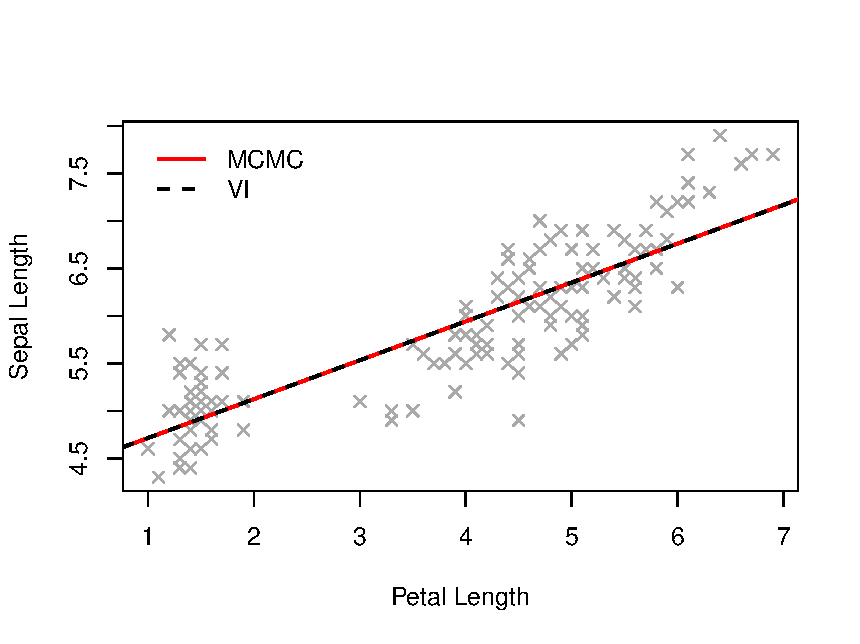
\includegraphics[scale=0.8]{Kap3/lrm_scatter.pdf}
    \caption{Scatterplot of sepal length (y-axis) against petal length (x-axis) for the \textit{Iris} dataset with estimated regression lines obtained via MCMC and VI.}
    \label{fig:lrm_scatter}
\end{figure}


Figure \ref{fig:lrm_scatter} shows similar results under both methodologies, and Table \ref{tab:fit_lr} provides a quantitative comparison of their performance. In particular, both MCMC and VI yield almost identical values for the information criteria (WAIC and DIC), as well as for the predictive accuracy metrics ($R^2$ and MSE). This confirms that the variational approximation provides an accurate posterior representation in this simple regression setting. However, a substantial difference arises in terms of computational efficiency: while MCMC requires approximately 21 seconds to complete, the VI method converges in about 1 second. This highlights one of the main advantages of variational inference, namely its ability to deliver results of comparable quality to MCMC but at a fraction of the computational cost.
 
\begin{table}[ht]
\centering
\caption{Goodness of fit and runtime (LRM, 1000 posterior samples), Iris Dataset.}
\label{tab:fit_lr}
\begin{tabular}{lrr}
\toprule
Metric & MCMC & VI \\
\midrule
WAIC & 160.061 & 160.259 \\
DIC & 160.028 & 160.215 \\
$R^2$ & 0.760 & 0.760 \\
MSE & 0.164 & 0.164 \\
Time (sec) & 21.184 & 1.008 \\
\bottomrule
\end{tabular}
\end{table}

\newpage

Figure \ref{fig:lrm_ELBO} illustrates the evolution of the Evidence Lower Bound (ELBO) as a function of execution time. The solid red curve corresponds to the VI optimization path, while the dashed blue line represents the posterior mean log-joint estimated via MCMC. As observed, the VI method rapidly increases the ELBO during the first iterations, reaching a stable plateau that closely approximates the MCMC benchmark within a fraction of a second. This behavior highlights the fast convergence properties of variational inference, which achieves a comparable approximation to the posterior distribution obtained by MCMC but with a substantially lower computational cost. In contrast, MCMC delivers a more robust estimate of the log-joint expectation, though at the expense of significantly longer execution time.


\begin{figure}[H]
    \centering
    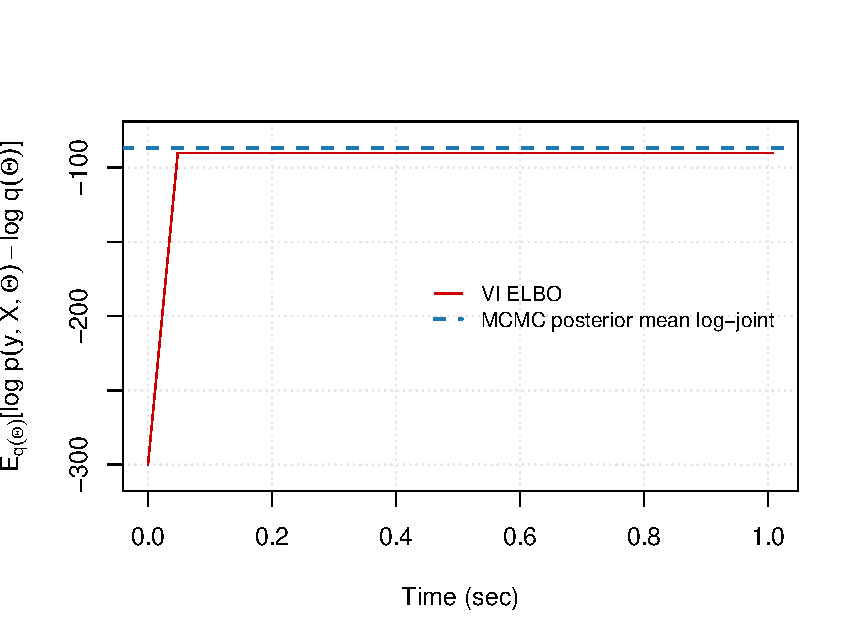
\includegraphics[scale=0.7]{Kap3/lrm_elbo_logjoint.pdf}
    \caption{Evolution of the ELBO compared with the posterior mean log-joint probability estimated via MCMC for LRM.}
    \label{fig:lrm_ELBO}
\end{figure}

Figure \ref{fig:lrm_betas_joint} presents the estimated joint posterior density for the regression coefficients 
$\bm{\beta} = (\beta_1, \beta_2)$ in the Iris dataset. The gray points correspond to MCMC draws, while the solid 
and dashed contours represent the $50\%$ and $95\%$ Mahalanobis credible regions obtained under MCMC and VI, 
respectively. Both methods yield highly consistent estimates of the joint distribution, with posterior means 
indicated by the vertical and horizontal lines. 

\vspace{0.5cm}

The overlap between the MCMC and VI contours indicates that the variational approximation is able to capture 
the main correlation structure between $\beta_1$ and $\beta_2$, as well as the shape and orientation of the 
joint posterior distribution. Moreover, the marginal credible intervals obtained from VI closely align with 
those derived from MCMC, demonstrating that in this setting the variational method achieves nearly the same 
precision as the MCMC approach, while offering substantial gains in computational efficiency.

\begin{figure}[H]
    \centering
    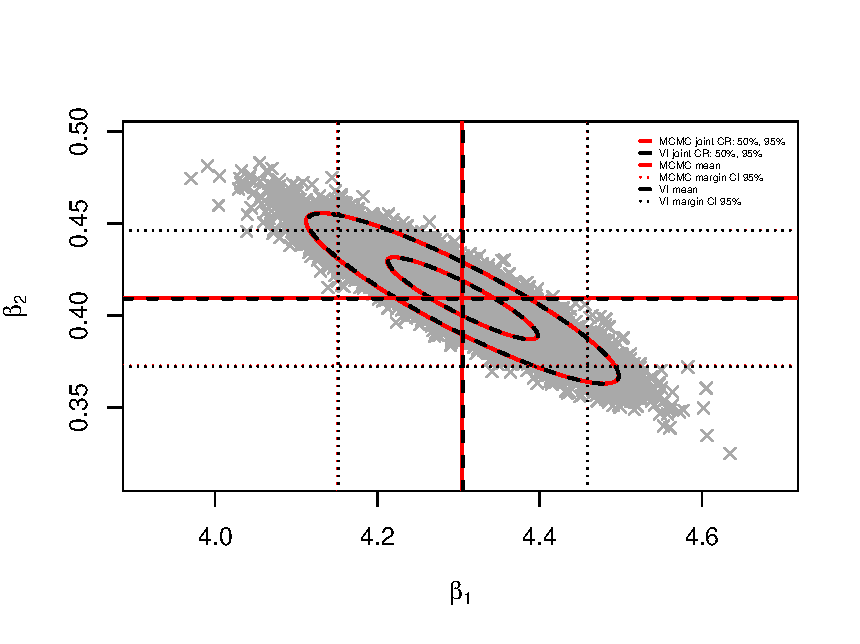
\includegraphics[scale=0.8]{Kap3/lrm_betas_joint.pdf}
    \caption{Joint posterior density estimates for $\bm{\beta} = (\beta_1, \beta_2)$ in the LRM using the Iris dataset, including Mahalanobis credible regions obtained via MCMC and VI and margin credible intervals.}
    \label{fig:lrm_betas_joint}
\end{figure}


\begin{figure}[H]
    \centering
    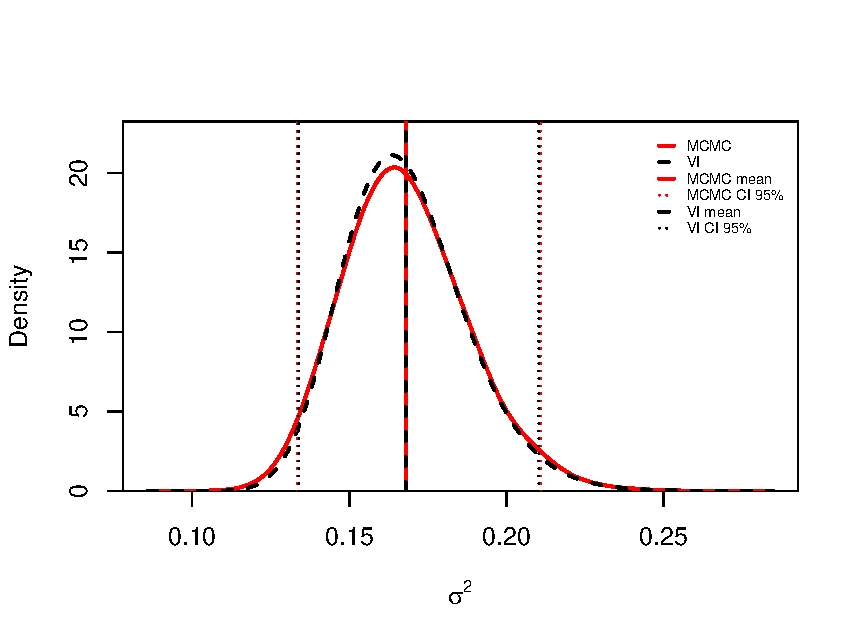
\includegraphics[scale=0.7]{Kap3/lrm_sigma2_density.pdf}
    \caption{Posterior density estimates for the error variance $\sigma^2$ in the LRM using the Iris dataset.}
    \label{fig:lrm_sigma2}
\end{figure}

\newpage

Figure \ref{fig:lrm_sigma2} shows the estimated posterior density of the error variance $\sigma^2$ under both 
MCMC and VI approaches. The two curves are nearly indistinguishable, with posterior means centered around 
$0.168$ and highly similar credible intervals. The vertical lines denote the posterior means, while the dotted 
lines correspond to the $95\%$ credible intervals under each method. Both approaches capture the uncertainty 
around $\sigma^2$ in a consistent manner, with VI closely approximating the posterior spread obtained from MCMC. 

\begin{table}[ht]
\centering
\caption{Posterior summaries LRM under MCMC and VI, Iris Dataset}
\label{tab:post_mcmc_vi}
\begin{tabular}{lcccccc}
\toprule
& \multicolumn{2}{c}{Mean} & \multicolumn{2}{c}{SD} & \multicolumn{2}{c}{CI} \\
\cmidrule(lr){2-3}\cmidrule(lr){4-5}\cmidrule(lr){6-7}
Parameter & MCMC & VI & MCMC & VI & MCMC & VI \\
\midrule
$\bm\beta_{1}$ & 4.305 & 4.306 & 0.079 & 0.078 & $[4.151, 4.458]$ & $[4.152, 4.459]$ \\
$\bm\beta_{2}$& 0.409 & 0.409 & 0.019 & 0.019 & $[0.373, 0.446]$ & $[0.372, 0.446]$ \\
$\sigma^2_{1}$ & 0.168 & 0.168 & 0.020 & 0.020 & $[0.133, 0.211]$ & $[0.134, 0.210]$ \\
\bottomrule
\end{tabular}
\end{table}

Table \ref{tab:post_mcmc_vi} further summarizes the posterior results. For $\sigma^2$, both methods report 
identical posterior means ($0.168$), standard deviations ($0.020$), and very similar $95\%$ credible intervals 
($[0.133,0.211]$ for MCMC versus $[0.134,0.210]$ for VI). These results confirm that, in this case, 
variational inference provides not only accurate point estimates but also a reliable approximation 
of posterior uncertainty relative to MCMC.

\subsubsection{Simulation}

With the purpose of assessing the performance of the proposed inference methodologies under controlled conditions, a simulation study was conducted in which each scenario is defined by the sample size $n$ and the number of predictors $p$, with true parameter values specified in the simulation design. For the case $p=3$, the regression coefficients were set to $\bm{\beta}=(25,10,-30)^\top$ with error variance $\sigma^2=100^2$, while for $p=2$ the coefficients were $\bm{\beta}=(2,-12)^\top$ with $\sigma^2=4^2$. Sample sizes $n=50,100,1000$ were considered for each configuration.

\vspace{0.5cm}

These configurations were chosen to evaluate the behavior of the inference methods across varying levels of model complexity and information content. In particular, increasing $n$ allows us to examine how the variational approximation improves as more data become available, while varying $p$ controls the dimensionality of the parameter space. Performance is assessed in terms of posterior mean accuracy, uncertainty quantification, and overall posterior approximation quality, using MCMC as a reference benchmark. Table~\ref{tab:method_quality} summarizes the performance of MCMC and VI across six simulation scenarios.

\begin{table}[ht]
\centering
\caption{Posterior zero coverage LRM under MCMC and VI in the $95\%$ CI, and runtime across simulation scenarios. }
\label{tab:method_quality}
\begin{tabular}{ccccccccc}
\toprule
 & & & \multicolumn{3}{c}{\textbf{MCMC}} & \multicolumn{3}{c}{\textbf{VI}} \\
\cmidrule(lr){4-6}\cmidrule(lr){7-9}
  n & p & \#params & $0 \in CI$ & Truth $\in $ CI & Time (s) & $0\in CI$ & Truth $\in$ CI & Time (s) \\

  50   & 3 & 4 & 3/4 (75.0\%)  & 4/4 (100.0\%) & 13.73 & 3/4 (75.0\%)  & 4/4 (100.0\%) & 0.59 \\
  100  & 3 & 4 & 3/4 (75.0\%)  & 4/4 (100.0\%) & 13.57 & 3/4 (75.0\%)  & 4/4 (100.0\%) & 0.59 \\
  1000 & 3 & 4 & 3/4 (75.0\%)  & 4/4 (100.0\%) & 14.67 & 3/4 (75.0\%)  & 4/4 (100.0\%) & 0.69 \\
  50   & 2 & 3 & 1/3 (33.3\%)  & 3/3 (100\%)  & 11.69 & 1/3 (33.3\%)  & 2/3 (66.7\%)  & 0.00 \\
  100  & 2 & 3 & 0/3 (0.0\%)   & 3/3 (100.0\%) & 11.80 & 0/3 (0.0\%)   & 3/3 (100.0\%) & 0.00 \\
  1000 & 2 & 3 & 0/3 (0.0\%)   & 3/3 (100.0\%) & 12.70 & 0/3 (0.0\%)   & 3/3 (100.0\%) & 0.00 \\
\bottomrule
\end{tabular}
\end{table}

\newpage

The metrics reported include (i) the proportion of parameters for which zero lies inside the $95\%$ posterior 
credible interval ($0 \in CI$), (ii) the proportion of true parameter values contained in the posterior 
credible interval (coverage), and (iii) the runtime in seconds. As expected, both methods exhibit perfect 
coverage of the true parameters across all scenarios ($100\%$ in almost all cases), while the presence of zero 
within the credible interval varies according to the underlying coefficients. This reflects the fact that the 
posterior distributions correctly exclude or include zero depending on whether the true effect is large or small. 

\vspace{0.5cm}

A striking difference appears in computational cost: MCMC requires between $11$ and $15$ seconds of execution 
time regardless of the sample size, while VI completes in less than one second for $p=3$ and virtually zero 
time for $p=2$. These results confirm that VI attains accuracy comparable to MCMC in terms of posterior 
coverage while offering substantial gains in computational efficiency, particularly in larger-scale settings.

\section{Hierarchical Normal Linear Regression Model}

The hierarchical linear models are extensions of linear regression models , where we can include a grouping structure present in data, as stated by
\cite{GELMAN}  , for examples persons within cities, students in schools, even repeated measures on the same individual. All of these cases present an hierarchical structure where the levels of these are taken as hierarchies, which implies that we can propose a linear regression where the regression coefficients can varying trough by group (Intercept and slopes). The inclusion of these structures can show a more accurately description and posterior inferences for the individuals, taking in account the specific information within the group and showing difference between groups.

\newpage

In \cite{HOFF} it describes the hierarchical linear model as a generalization of normal hierarchical model where we can compare multiple groups taking account the heterogeneity across several populations and  heterogeneity within the groups even including an specific behavior per group, to extend the results, the ordinary regression model is used to describe within-group heterogeneity of observations, then describe between-group heterogeneity using a sampling model for the group-specific regression parameters,as follows:

\begin{equation}
\label{HRLM}
y_{ij} \mid \bm{x}_{ij}, \bm{\beta}_j, \sigma_j^2 \stackrel{\text { ind }}{\sim} \mathsf{N}\left(\bm{x}_{ij}^{\bm{\top}} \bm{\beta}_j, \sigma_j^2\right), \quad i=1, \ldots, n_j, \quad j=1, \ldots, m
\end{equation}

Where $\bm{x}_{ij}$ is a $p \times 1$ vector of regressors for observation $i$ in group $j$,  $\bm{y}_j = \left[y_{1j}, \ldots, y_{n_j, j}\right]^\top$  is a $n_j \times 1$ vector of response variable values for group $j$  and $\mathbf{X}_j = \left[\bm{x}_{1j}, \ldots, \bm{x}_{n_j, j}\right]^\top$ a $n_j \times p$ matrix , the within-group sampling model can be expressed equivalently as $\bm{y}_j \sim$  $\mathsf{N_p}\left(\mathbf{X}_j \bm{\beta}_j, \sigma^2_j \mathbf{I}_p\right)$, with the group-specific data vectors $\bm{y}_1, \ldots, \bm{y}_m$ being conditionally independent given all $\bm{\beta}_j$ and $\sigma^2_j$.

\subsection{Prior Distributions}

In order to specify a Bayesian point of view to estimate the parameters   \cite{SOSA} propose define the priors distributions for the parameters vector $\bm{\Theta}=(\bm{\xi},\bm{\sigma^2},\bm{\beta},\bm{\Sigma},\xi^2)$ with $\bm{\xi}=(\bm{\beta}_1, \ldots, \bm{\beta}_m)$,    $\bm{\beta}_j=(\beta_{1j},\cdots,\beta_{pj})$ and $\bm{\sigma^2}=(\sigma_1^2,\cdots,\sigma_m^2)$  for model described in figure \ref{HRLM} represented by \ref{fig:DAG_HLRM}, as follows:

\begin{equation}
    \label{hyper_HRLM_1}
    \bm{\beta}_j \mid \bm{\beta}, \bm{\Sigma} \stackrel{\mathsf{iid}}{\sim} \mathsf{N}_p(\bm{\beta}, \bm{\Sigma}) \quad \text { and } \quad \sigma_j^2 \mid \xi^2 \stackrel{\mathsf{iid}}{\sim} \mathsf{IG}\left(\nu_0 / 2, \nu_0 \xi^2 / 2\right)
\end{equation}

\begin{equation}
    \label{hyper_HRLM_2}
    \bm{\beta} \sim \mathsf{N_p}\left(\bm{\mu}_0, \bm{\Lambda}_0\right), \quad \bm{\Sigma} \sim \mathsf{IW}\left(n_0, \mathbf{S}_0^{-1}\right), \quad \xi^2 \sim \mathsf{G}\left(a_0, b_0\right)
\end{equation}

with $\bm{\mu}_0, \bm{\Lambda}_0, n_0, \mathbf{S}_0, \nu_0, a_0, \text { and } b_0$ the hyperparameters of model.

\begin{figure}[H]
    \centering
    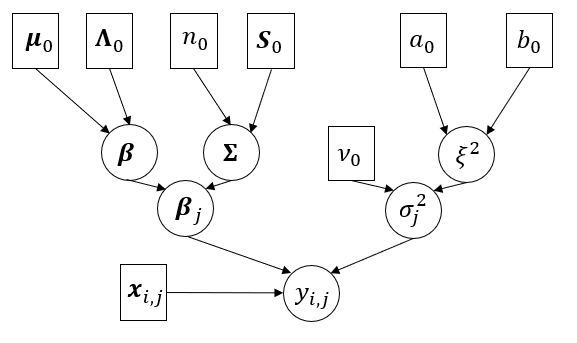
\includegraphics[scale=0.8]{Kap2/DAG_HLRM.png}
    \caption{DAG Representation HLRM}
    \label{fig:DAG_HLRM}
\end{figure}

\subsubsection{Prior Elicitation}

\cite{KassWasserman1995} and \cite{SOSA} adopt the unit–information–prior perspective, under which the hyperparameters for the HLRM are specified to yield a weak but coherent prior configuration. In particular, we define $g = \sum_{j=1}^{m} n_j$ and fix $\nu_0 = 1$, while the location parameter is taken as $\bm{\mu}_0 = \hat{\bm{\beta}}_{\text{OLS}}$. The scale matrix is set to $\bm{\Lambda}_0 = g\,\hat{\sigma}^2_{\text{OLS}}(\bm{X}^\top\bm{X})^{-1}$, with $\hat{\sigma}^2_{\text{OLS}}$ denoting the residual variance from the OLS fit. For the covariance hyperparameters, we choose $n_0 = p + 2$ and $\bm{S}_0 = \bm{\Lambda}_0$, a combination that produces a diffuse yet centered concentration around $\bm{\mu}_0$. Lastly, for the variance component, the settings $a_0 = 1$ and $b_0 = 1/\hat{\sigma}^2_{\text{OLS}}$ are adopted, ensuring that $\mathsf{E}(\xi^2) = \hat{\sigma}^2_{\text{OLS}}$, which produces a diffuse prior.

\subsection{Posterior Inference}

\subsubsection{Gibbs Sampling}

Once again we derivate the f.c.d's for each parameter in $\bm{\Theta}=(\bm{\zeta},\bm{\sigma^2},\bm{\beta},\bm{\Sigma},\xi^2)$ starting from the full posterior distribution, this is:

\begin{equation}
\begin{split}
    \label{POST_HLRM}
    p(\bm{\Theta} \mid\bm{y}, \bm{X}) 
    &\propto p(\bm{y} \mid \bm{X}, \bm{\zeta} ,\bm{\sigma^2}) 
p(\bm{\zeta} \mid \bm{\beta}, \bm{\Sigma}) 
p(\bm{\beta}) 
p(\bm{\Sigma}) 
p(\bm{\sigma^2}\mid 
\xi^2)
p(\xi)\\
&\propto \prod_{j=1}^{m}\mathsf{N}_{n_j}(\bm{y}_{j}\mid\bm{X}_{j} \bm{\beta}_j,{\sigma}_j^2)\times\prod_{j=1}^{m}\mathsf{N_p}(\bm{\beta}_j \mid \bm{\beta}, \bm{\Sigma})\times\mathsf{N_p}(\bm{\beta}\mid\bm{\mu}_0, \bm{\Lambda}_0)\\
&\quad\times\mathsf{IW}\left(\bm{\Sigma}\mid n_0, \mathbf{S}_0^{-1}\right)\times\prod_{j=1}^{m}\mathsf{IG}\left(\sigma_j^2 \mid\nu_0 / 2, \nu_0 \xi^2 / 2\right)\times\mathsf{G}\left(\xi^2 \mid a_0, b_0\right)\\
&\propto \prod_{j=1}^{m}  ({\sigma}_j^2)^{-n_j/2} 
\exp\left\{ -\frac{1}{2\sigma_j^2} (\bm{y}_{j} - \bm{X}_{j} \bm{\beta}_j)^\top(\bm{y}_{j} - \bm{X}_{j} \bm{\beta}_j) \right\} \\
&\quad\times \prod_{j=1}^{m} \left| \bm{\Sigma} \right|^{-1/2} 
\exp\left\{ -\frac{1}{2} (\bm{\beta}_j -  \bm{\beta})^\top \bm{\Sigma}^{-1} (\bm{\beta}_j - \bm{\beta}) \right\} \\
&\quad \times \exp\left\{ -\frac{1}{2} (\bm{\beta} - \bm{\mu}_0)^\top \bm{\Lambda}_0^{-1} (\bm{\beta} - \bm{\mu}_0) \right\}
\times |\bm{\Sigma}|^{-(n_0 + p + 1)/2} 
 \exp\left\{ -\frac{1}{2} \mathrm{tr}(\bm{S}_0 \bm{\Sigma}^{-1}) \right\} \\
&\quad \times \prod_{j=1}^{m} (\xi^2)^{\nu_0 / 2 - 1} 
(\sigma_j^2)^{-(\nu_0 / 2+1)} 
\exp\left\{ -\frac{\nu_0 \xi^2}{2 \sigma_j^2} \right\} 
\times (\xi^2)^{a_0 - 1} \exp\left\{ -b_0 \xi^2 \right\}
\end{split}
\end{equation}

then, the f.c.d.s for this model are:

\begin{itemize}
    \item f.c.d of $\bm{\beta}_j$ for $j=1,\dots,m$
    \begin{equation}
        \label{HLRM_MCMC_Betaj}
        \bm{\beta}_j \mid \text{rest} \sim \mathsf{N_p} \left( 
\left[ ({\sigma_j}^{-2}) \bm{X}_{j} \bm{X}_{j}^\top + \bm{\Sigma}^{-1} \right]^{-1}
\left[ ({\sigma_j}^{-2}) \bm{X}_{j}^\top \bm{y}_{j} + \bm{\Sigma}^{-1} \bm{\beta} \right], \ 
\left[ (\sigma_j^{-2}) \bm{X}_{j} \bm{X}_{j}^\top  + \bm{\Sigma}^{-1} \right]^{-1}
\right)
    \end{equation}
    \item f.c.d of $\bm{\beta}$
    \begin{equation}
        \label{HLRM_MCMC_Beta}
        \bm{\beta} \mid \text{rest} \sim \mathsf{N}_p \left(
\left( \bm{\Lambda}_0^{-1} + m \bm{\Sigma}^{-1} \right)^{-1}
\left( \bm{\Lambda}_0^{-1} \bm{\mu}_0 + \bm{\Sigma}^{-1} \sum_{j=1}^{m} \bm{\beta}_j \right),
\left( \bm{\Lambda}_0^{-1} + m \bm{\Sigma}^{-1} \right)^{-1}\right)
    \end{equation}
    \item f.c.d of $\bm{\Sigma}$
    \begin{equation}
        \label{HLRM_MCMC_Sigma}
        \bm{\Sigma} \mid \text{rest} \sim \mathsf{IW} \left( 
n_0 + m,\ 
\left( \bm{S}_0 + \sum_{j=1}^{m} (\bm{\beta}_j - \bm{\beta})(\bm{\beta}_j - \bm{\beta})^\top\right)^{-1}
\right)
    \end{equation}
    
\item f.c.d of $\sigma_j^2$ for $j=1,\dots,m$
    
    \begin{equation}
        \label{HLRM_MCMC_sigma2j}
        \sigma_j^2 \mid \text{rest} \sim \mathsf{IG} \left( 
\frac{n_j + \nu_0}{2},\ 
\frac{ \nu_0 \xi^2 +  (\bm{y}_{j} - \bm{X}_{j} \bm{\beta}_j)^\top(\bm{y}_{j} - \bm{X}_{j} \bm{\beta}_j)}{2} 
\right)
    \end{equation}
    \item f.c.d of $\xi^2$
    \begin{equation}
        \label{HLRM_MCMC_xi2}
        \xi^2 \mid \text{rest} \sim \mathsf{G} \left(
\frac{m \nu_0}{2} + a_0,\ 
b_0 + \frac{\nu_0}{2} \sum_{j=1}^{m} \sigma_j^{-2}
\right)
    \end{equation}
\end{itemize}

\begin{algorithm}[H]
\caption{Gibbs Sampling for HLRM}
\begin{algorithmic}
\State \textbf{Input} Init values $\{\bm{\beta}_j^{(0)}\}_{j=1}^m,\; \bm{\beta}^{(0)},\; \bm{\Sigma}^{(0)},\; \{\sigma_j^{2(0)}\}_{j=1}^m,\; \xi^{2(0)}$, hyperparameters $\bm{\mu}_0,\bm{\Lambda}_0, n_0,\bm{S}_0,a_0,b_0,\nu_0,\sigma_0^2$, data values $\{\bm{y}_j,\bm{X}_j\}_{j=1}^m$

\For{$b = 1, \dots, B$}
  \For{$j = 1, \dots, m$}
    \State Sample $\bm{\beta}_j^{(b)} \sim p\!\left(\bm{\beta}_j \mid \bm{\beta}^{(b-1)},\bm{\Sigma}^{(b-1)},(\sigma_j^2)^{(b-1)},\bm{y}_j,\bm{X}_j\right)$ from eq. \ref{HLRM_MCMC_Betaj}
    \State Sample $(\sigma_j^2)^{(b)} \sim p\!\left(\sigma_j^2 \mid \bm{\beta}_j^{(b)},(\xi^2)^{(b-1)},\bm{y}_j,\bm{X}_j\right)$ from eq. \ref{HLRM_MCMC_sigma2j}
  \EndFor
  \State Sample $\bm{\beta}^{(b)} \sim p\!\left(\bm{\beta} \mid \{\bm{\beta}_j^{(b)}\},\bm{\Sigma}^{(b-1)}\right)$ from eq. \ref{HLRM_MCMC_Beta}
  \State Sample $\bm{\Sigma}^{(b)} \sim p\!\left(\bm{\Sigma} \mid \{\bm{\beta}_j^{(b)}\},\bm{\beta}^{(b)}\right)$ from eq. \ref{HLRM_MCMC_Sigma}
  \State Sample $(\xi^2)^{(b)} \sim p\!\left(\xi^2 \mid \{(\sigma_j^2)^{(b)}\}\right)$ from eq. \ref{HLRM_MCMC_xi2}
\EndFor
\State \textbf{Output} Draws $\{\bm{\beta}_j^{(b)},(\sigma_j^2)^{(b)},\bm{\beta}^{(b)},\bm{\Sigma}^{(b)},(\xi^2)^{(b)}\}_{b=1}^B$
\end{algorithmic}
\end{algorithm}

For detailed and explicit derivations of these results, see Appendix \ref{Appendix_B}.

\subsubsection{CAVI}

As before, we define the variational distribution to approximate the posterior distribution under the mean–field assumption described in result \ref{MFA}. Using the CAVI results for exponential family models in \ref{NMVFB_opt}, we derive the variational parameters for each factor. It is important to note that these variational parameters can be decomposed into local parameters, which are specific to each group $j$, and global parameters, which correspond to latent variables shared across all groups.


\begin{equation}
\label{Q_HLRM}
\begin{split}
q(\bm{\Theta})&=\prod_{j=1}^{m}q(\bm{\beta}_j)q(\bm{\beta})q(\bm{\Sigma})\prod_{j=1}^{m}q(\sigma_j^2)q(\xi^2)\\
&= \left(\prod_{j=1}^{m}q(\bm{\beta}_j)q(\sigma_j^2)\right)\left(q(\bm{\beta})q(\bm{\Sigma})q(\xi^2)\right)
\end{split}
\end{equation}

\begin{itemize}
    \item Factor $q(\bm{\beta}_j)=\mathsf{N_p}(\bm{\mu}_{\bm{\beta}_j},\bm{\Sigma}_{\bm{\beta}_j})$  for $j=1,\dots,m$, with

\begin{equation}
\label{HLRM_CAVI_Sigma_Betaj}
\bm{\Sigma}_{\bm{\beta}_j} = \left[ \mathsf{E}_{\sigma^2_j}\left[{\sigma_j}^{-2}\right] \bm{X}_{j} \bm{X}_{j}^\top  + \mathsf{E}_{\bm{\Sigma}}\left[\bm{\Sigma}^{-1}\right]  \right]^{-1},
\end{equation}

\begin{equation}
\label{HLRM_CAVI_Mu_Betaj}
\bm{\mu}_{\bm{\beta}_j}= \left[ \mathsf{E}_{\sigma^2_j}\left[{\sigma_j}^{-2}\right] \bm{X}_{j} \bm{X}_{j}^\top  + \mathsf{E}_{\bm{\Sigma}}\left[\bm{\Sigma}^{-1}\right]  \right]^{-1}\left[\mathsf{E}_{\sigma^2_j}\left[{\sigma_j}^{-2}\right] \bm{X}_{j}^\top \bm{y}_{j} + \mathsf{E}_{\bm{\Sigma}}\left[\bm{\Sigma}^{-1}\right] \mathsf{E}_{\bm{\beta}}\left[\bm{\beta} \right] \right]
\end{equation}

\item Factor $q(\bm{\beta})=\mathsf{N_p}(\bm{\mu}_{\bm{\beta}},\bm{\Sigma}_{\bm{\beta}})$, with

\begin{equation}
\label{HLRM_CAVI_Sigma_Beta}
\bm{\Sigma}_{\bm{\beta}} = \left[\bm{\Lambda}_0^{-1}   + \sum_{j=1}^{m}\mathsf{E}_{\bm{\Sigma}}\left[\bm{\Sigma}^{-1}\right]  \right] ^{-1},
\end{equation}

\begin{equation}
\label{HLRM_CAVI_Mu_Beta}
\bm{\mu}_{\bm{\beta}}= \left[\bm{\Lambda}_0^{-1}   + \sum_{j=1}^{m}\mathsf{E}_{\bm{\Sigma}}\left[\bm{\Sigma}^{-1}\right]  \right]^{-1}\left[\bm{\Lambda}_0^{-1} \bm{\mu}_0 + \sum_{j=1}^{m}\mathsf{E}_{\bm{\Sigma}}\left[\bm{\Sigma}^{-1}\right] \mathsf{E}_{\bm{\beta}_j}\left[\bm{\beta}_j \right]\right]
\end{equation}

    \item Factor $q(\bm{\Sigma})=\mathsf{IW}(\nu_{\bm{\Sigma}},\bm{S}_{\bm{\Sigma}}^{-1})$, with

\begin{equation}
\label{HLRM_CAVI_nu_Sigma}
\nu_{\bm{\Sigma}} = n_0+m,
\end{equation}

\begin{equation}
\label{HLRM_CAVI_S_Sigma}
\bm{S}_{\bm{\Sigma}}=  \bm{S}_0 + \sum_{j=1}^{m} \mathsf{E}_{\bm{\beta}_j,\bm{\beta}}\left[\left(\bm{\beta}_j - \bm{\beta})(\bm{\beta}_j - \bm{\beta}\right)^\top\right]
\end{equation}
    
    \item Factor $q(\sigma_j^2)=\mathsf{IG}(a_{\sigma_j^2},b_{\sigma_j^2})$ for $j=1,\dots,m$, with

\begin{equation}
\label{HLRM_CAVI_a_sigma2j}
a_{\sigma_j^2}= \frac{n_j + \nu_0}{2},
\end{equation}

\begin{equation}
\label{HLRM_CAVI_b_sigma2j}
b_{\sigma_j^2}= \frac{ \nu_0 \mathsf{E}_{\xi^2}\left[\xi^2\right] +  \mathsf{E}_{\bm{\beta}_j}\left[\left(\bm{y}_{j} - \bm{X}_{j} \bm{\beta}_j)^\top(\bm{y}_{j} - \bm{X}_{j} \bm{\beta}_j\right)\right]}{2}
\end{equation}

    \item Factor $q(\xi^2)=\mathsf{G}(a_{\xi^2},b_{\xi^2})$, with

\begin{equation}
\label{HLRM_CAVI_a_xi2}
a_{\xi^2}=  a_0 +\frac{m \nu_0}{2},
\end{equation}

\begin{equation}
\label{HLRM_CAVI_b_xi2}
b_{\xi^2}= b_0 + \frac{\nu_0}{2} \sum_{j=1}^{m} \mathsf{E}_{\sigma^2_j}\left[\sigma_j^{-2}\right]
\end{equation}

\item ELBO $\mathcal{L}(q(\bm{\Theta}))$

\begin{equation}
\label{HLRM_CAVI_ELBO}
\begin{split}
\mathcal{L}(q(\bm{\Theta}))
&=\mathsf{E}_{\bm{\Theta}}\left[\log p(\bm{\Theta},\bm{y}, \bm{X})\right]-\mathsf{E}_{\bm{\Theta}}\left[\log q(\bm{\Theta})\right]\\
&= \sum_{j=1}^{m} \mathsf{E}_{\bm{\Theta}}\left[\log p\left(\bm{y}_j \mid \bm{\beta}_j, \sigma_j^2, \mathbf{X}_j \right)\right]+\sum_{j=1}^{m} \left(\mathsf{E}_{\bm{\Theta}}\left[\log p\left(\bm{\beta}_j \mid \bm{\beta}, \bm{\Sigma}\right)\right]-\mathsf{E}_{\bm{\beta}_j}\left[\log q(\bm{\beta}_j)\right]\right) \\ 
&\quad + \left(\mathsf{E}_{\bm{\Theta}}\left[\log p(\bm{\beta})\right]-\mathsf{E}_{\bm{\beta}}\left[\log q\left(\bm{\beta}\right)\right]\right)+\left(\mathsf{E}_{\bm{\Theta}}\left[\log p\left(\bm{\Sigma}\right)\right]- \mathsf{E}_{\bm{\Sigma}}\left[\log q(\bm{\Sigma})\right]\right) \\
&\quad + \sum_{j=1}^{m} \left(\mathsf{E}_{\bm{\Theta}}\left[\log p\left(\sigma^2_j\mid\xi^2\right)\right]-\mathsf{E}_{\sigma^2_j}\left[\log q\left(\sigma^2_j\right) \right]\right) + \left(\mathsf{E}_{\bm{\Theta}}\left[\log p(\xi^2)\right] - \mathsf{E}_{\xi^2}\left[\log q(\xi^2)\right]\right)
\end{split}
\end{equation}

where:

\begin{itemize}

\item
$
\begin{aligned}
\mathsf{E}_{\bm{\Theta}}\left[\log p\left(\bm{y}_j \mid \bm{\beta}_j, \sigma_j^2, \mathbf{X}_j \right)\right]
&= -\tfrac{n_j}{2}\log(2\pi)
-\tfrac{n_j}{2}\left(\log b_{\sigma_j^2}-\psi(a_{\sigma_j^2})\right) \\
&\quad -\tfrac{1}{2}\left(\tfrac{a_{\sigma_j^2}}{b_{\sigma_j^2}}\right)
\Big[
(\bm{y}_j-\mathbf{X}_j\bm{\mu}_{\bm{\beta}_j})^\top(\bm{y}_j-\mathbf{X}_j\bm{\mu}_{\bm{\beta}_j})
+\operatorname{tr}\!\left(\mathbf{X}_j^\top\mathbf{X}_j\,\bm{\Sigma}_{\bm{\beta}_j}\right)
\Big]
\end{aligned}
$

\item
$
\begin{aligned}
\mathsf{E}_{\bm{\Theta}}\left[\log p\left(\bm{\beta}_j \mid \bm{\beta}, \bm{\Sigma}\right)\right]
&= -\tfrac{p}{2}\log(2\pi)
-\tfrac{1}{2}\Bigg(
-\sum_{i=1}^{p}\psi\left(\tfrac{\nu_{\bm{\Sigma}}+1-i}{2}\right)
-p\log 2 + \log|\bm{S}_{\bm{\Sigma}}^{-1}|
\Bigg) \\
&\qquad -\tfrac{1}{2}\operatorname{tr}\left(\bm{S}_{\bm{\Sigma}}^{-1}\left[
(\bm{\mu}_{\bm{\beta}_j}-\bm{\mu}_{\bm{\beta}})
(\bm{\mu}_{\bm{\beta}_j}-\bm{\mu}_{\bm{\beta}})^\top
+\bm{\Sigma}_{\bm{\beta}_j}+\bm{\Sigma}_{\bm{\beta}}
\right]\right)
\end{aligned}
$

\item
$
\mathsf{E}_{\bm{\beta}_j}\left[\log q(\bm{\beta}_j)\right]
= -\tfrac{p}{2}\log(2\pi e)-\tfrac{1}{2}\log|\bm{\Sigma}_{\bm{\beta}_j}|
$

\item
$
\begin{aligned}
\mathsf{E}_{\bm{\Theta}}\left[\log p(\bm{\beta})\right]
&= -\tfrac{p}{2}\log(2\pi)-\tfrac{1}{2}\log|\bm{\Lambda}_0| -\tfrac{1}{2}\left[
(\bm{\mu}_{\bm{\beta}}-\bm{\mu}_0)^\top\bm{\Lambda}_0^{-1}(\bm{\mu}_{\bm{\beta}}-\bm{\mu}_0)
+\operatorname{tr}\!\left(\bm{\Lambda}_0^{-1}\bm{\Sigma}_{\bm{\beta}}\right)
\right]
\end{aligned}
$

\item
$
\mathsf{E}_{\bm{\beta}}\left[\log q\left(\bm{\beta}\right)\right]
= -\tfrac{p}{2}\log(2\pi e)-\tfrac{1}{2}\log|\bm{\Sigma}_{\bm{\beta}}|
$

\item
$
\begin{aligned}
\mathsf{E}_{\bm{\Theta}}\left[\log p\left(\bm{\Sigma}\right)\right]
&= \tfrac{n_0}{2}\log|\bm{S}_0|-\tfrac{n_0 p}{2}\log 2-\log\Gamma_p\left(\tfrac{n_0}{2}\right)  -\tfrac{n_0+p+1}{2}\Bigg(
-\sum_{i=1}^{p}\psi\!\left(\tfrac{\nu_{\bm{\Sigma}}+1-i}{2}\right)-p\log 2+\log|\bm{S}_{\bm{\Sigma}}^{-1}|
\Bigg) \\
&\quad -\tfrac{1}{2}\operatorname{tr}\left(\bm{S}_0\,\bm{S}_{\bm{\Sigma}}^{-1}\right)
\end{aligned}
$

\item
$
\begin{aligned}
\mathsf{E}_{\bm{\Sigma}}\left[\log q(\bm{\Sigma})\right]
&= \tfrac{\nu_{\bm{\Sigma}}}{2}\log|\mathbf{S}_{\bm{\Sigma}}|
- \tfrac{\nu_{\bm{\Sigma}} p}{2}\log 2
- \log\Gamma_p\left(\tfrac{\nu_{\bm{\Sigma}}}{2}\right)  - \tfrac{\nu_{\bm{\Sigma}}+p+1}{2}\left(
-\sum_{i=1}^{p}\psi\left(\tfrac{\nu_{\bm{\Sigma}}+1-i}{2}\right)-p\log 2+\log|\mathbf{S}_{\bm{\Sigma}}^{-1}|
\right) \\
&\quad - \tfrac{\nu_{\bm{\Sigma}}}{2}\operatorname{tr}\left(\mathbf{S}_{\bm{\Sigma}}^2\right)
\end{aligned}
$

\item
$
\begin{aligned}
\mathsf{E}_{\bm{\Theta}}\left[\log p\left(\sigma^2_j\mid\xi^2\right)\right]
&= \tfrac{\nu_0}{2}\log\left(\tfrac{\nu_0}{2}\right)
+\tfrac{\nu_0}{2}\left(\psi(a_{\xi^2})-\log b_{\xi^2}\right)
-\log\Gamma\!\left(\tfrac{\nu_0}{2}\right)-\left(\tfrac{\nu_0}{2}+1\right)\left(\log b_{\sigma_j^2}-\psi(a_{\sigma_j^2})\right) \\
&\quad -\tfrac{\nu_0}{2}\left(\tfrac{a_{\xi^2}}{b_{\xi^2}}\right)\left(\tfrac{a_{\sigma_j^2}}{b_{\sigma_j^2}}\right)
\end{aligned}
$

\item
$
\mathsf{E}_{\sigma^2_j}\left[\log q\left(\sigma^2_j\right) \right]
= -\log b_{\sigma_j^2}-\log\Gamma(a_{\sigma_j^2})+(a_{\sigma_j^2}+1)\psi(a_{\sigma_j^2})-a_{\sigma_j^2}
$

\item
$
\mathsf{E}_{\bm{\Theta}}\left[\log p(\xi^2)\right]
= a_0\log b_0-\log\Gamma(a_0)
+(a_0-1)\left(\psi(a_{\xi^2})-\log b_{\xi^2}\right)
-b_0\left(\tfrac{a_{\xi^2}}{b_{\xi^2}}\right)
$

\item
$
\mathsf{E}_{\xi^2}\left[\log q(\xi^2)\right]
= \log b_{\xi^2}-\log\Gamma(a_{\xi^2})+(a_{\xi^2}-1)\psi(a_{\xi^2})-a_{\xi^2}
$

\end{itemize}


\end{itemize}

\begin{algorithm}[H]
\caption{CAVI for HLRM}
\label{CAVI_HLRM_alg}
\begin{algorithmic}
\State \textbf{Input} Init values $\{\bm{\mu}_{\beta_j}^{(0)}, \bm{\Sigma}_{\beta_j}^{(0)}\}_{j=1}^m,\bm{\mu}_\beta^{(0)},\bm{\Sigma}_\beta^{(0)},\nu_{\bm{\Sigma}},\bm{S}_\Sigma^{(0)},a_\xi^{(0)}, b_\xi^{(0)},a_{\sigma_j^2}^{(0)}, b_{\sigma_j^2}^{(0)}$, hyperparameters $\bm{\mu}_0,\bm{\Lambda}_0,n_0,\bm{S}_0,a_0,b_0,\nu_0,\sigma_0^2$, data values $\{\bm{y}_j,\bm{X}_j\}_{j=1}^m$

\While{ELBO not converged}
  \For{$j = 1,\dots,m$}
  \State \textbf{\textit{Local updates}}
    \State Update $q (\bm{\beta}_j)$ setting $\bm{\Sigma}_{\bm{\beta}_j}$ (eq. \ref{HLRM_CAVI_Sigma_Betaj})  and $\bm{\mu}_{\bm{\beta}_j}$ (eq. \ref{HLRM_CAVI_Mu_Betaj}) .
\State Update $q(\sigma^2_j)$ setting $a_{\sigma_j^2}$ (eq. \ref{HLRM_CAVI_a_sigma2j}) and $b_{\sigma_j^2}$ (eq. \ref{HLRM_CAVI_a_sigma2j}).
  \EndFor
  \State \textbf{\textit{Global updates}}
    \State Update $q (\bm{\Sigma})$ setting $\bm{S}_{\bm{\Sigma}}$ (eq. \ref{HLRM_CAVI_S_Sigma}).
  \State Update $q (\bm{\beta})$ setting $\bm{\mu}_{\bm{\beta}}$ (eq. \ref{HLRM_CAVI_Mu_Beta}) and $\bm{\Sigma}_{\bm{\beta}}$ (eq. \ref{HLRM_CAVI_Sigma_Beta}) .
  \State Update $q (\xi^2)$ setting $a_{\xi^2}$ (eq. \ref{HLRM_CAVI_a_xi2}) and $b_{\xi^2}$ (eq. \ref{HLRM_CAVI_b_xi2}).
\State Calculate ELBO $\mathcal{L}(q(\bm{\Theta}))$ (eq. \ref{HLRM_CAVI_ELBO}).
\EndWhile
\State \textbf{Output} Optimal parameters $\{\bm{\mu}_{\beta_j}, \bm{\Sigma}_{\beta_j}\}_{j=1}^m,\bm{\mu}_\beta,\bm{\Sigma}_\beta,\nu_{\bm{\Sigma}},\bm{S}_\Sigma,a_{\xi^2}, b_{\xi^2},a_{\sigma_j^2}, b_{\sigma_j^2}$
\end{algorithmic}
\end{algorithm}

\subsubsection{SVI}

Since the hierarchical linear regression model  previously discussed satisfies the assumptions of
the stochastic variational inference algorithm (see subsection \ref{SVI}), it is straightforward to derive the required
updates via the Robbins–Monro optimization scheme (see \ref{Robbins-Monro}) from equations (\ref{HLRM_CAVI_Sigma_Betaj}) to (\ref{HLRM_CAVI_b_xi2}). The resulting algorithm is described below in \ref{SVI_HLRM_alg}.

\subsection{Illustration}
\subsubsection{Farms Dataset}
\label{farms}
The methodologies developed in this work are illustrated through an application 
to an agricultural dataset involving measurements of soil nitrogen and plant size. 
The dataset, originally discussed in \cite{Crawley2012}, consists of $m=24$ farms, 
each providing $n=5$ paired observations of local soil nitrogen concentration ($N$) 
and corresponding plant size. Thus, for each farm $j=1,\dots,24$, we observe 
$\{(N_{ij}, S_{ij}) : i=1,\dots,5\}$, where $S_{ij}$ denotes the plant size and $N_{ij}$ 
the soil nitrogen level. The scientific motivation underlying this study is the 
established role of nitrogen as an essential macro-nutrient for plant development, 
with higher levels typically associated with increased growth and yield, though 
excessive levels may have detrimental effects. 

\begin{algorithm}[H]
\caption{SVI for HLRM}
\begin{algorithmic}
\State \textbf{Input} Init values $
\bm{\mu}_{\bm{\beta}}^{(0)},\; \bm{\Sigma}_{\bm{\beta}}^{(0)},\nu_{\bm{\Sigma}}, \bm{S}_{\bm{\Sigma}}^{(0)},\; a_{\sigma_j^2}^{(0)}, b_{\sigma_j^2}^{(0)},\; a_{\xi^2}, b_{\xi^2}^{(0)}$, hyperparameters $\bm{\mu}_0,\bm{\Lambda}_0,n_0,\bm{S}_0,a_0,b_0,\nu_0,\sigma_0^2$, learning rate parameters $\tau,\chi$, minibatch size $|\mathcal{S}|$, number of iterations $T$

\For{$t = 1,\dots,T$}
    \State \textbf{\textit{Local updates}}
  \State Select a mini-batch of groups $\mathcal{S} \subset \{1,\dots,m\}$.

  \For{$j \in \mathcal{S}$}

    \State Update $q(\bm{\beta}_j)$ setting $\bm{\mu}_{\bm{\beta}_j}^{(t)}$ (eq. \ref{HLRM_CAVI_Mu_Betaj}) and $\bm{\Sigma}_{\bm{\beta}_j}^{(t)}$ (eq. \ref{HLRM_CAVI_Sigma_Betaj}).
\State Update $q(\sigma^2_j)$ setting $a_{\sigma_j^2}^{(t)}$ (eq. \ref{HLRM_CAVI_a_sigma2j} ) and $b_{\sigma_j^2}^{(t)}$ (eq. \ref{HLRM_CAVI_a_sigma2j}).
  \EndFor
  \State Calculate $\rho_t = (t+\tau)^{-\chi}$
   \State \textbf{\textit{Noisy Gradients}}
  \State Calculate Intermediate global parameters
   $$
  \hat{\bm{\Sigma}_{\bm{\beta}}}^{-1} =\bm{\Lambda}_0^{-1} + \tfrac{m}{|\mathcal{S}|}\sum_{j \in \mathcal{S}} \mathsf{E}_{\bm{\Sigma}}\left[\bm{\Sigma}^{-1}\right], \quad \hat{\bm{\mu}_{\bm{\beta}}} = \hat{\bm{\Sigma}_{\bm{\beta}}}\left(\bm{\Lambda}_0^{-1}\bm{\mu}_0 + \tfrac{m}{|\mathcal{S}|}\sum_{j \in \mathcal{S}}
  \mathsf{E}_{\bm{\Sigma}}\left[\bm{\Sigma}^{-1}\right]
  \mathsf{E}_{\bm{\beta}_j}\left[\bm{\beta}_j \right]\right) 
  $$
  
  $$
  \hat{\bm{S}_{\bm{\Sigma}}} = \bm{S}_0 +\tfrac{m}{|\mathcal{S}|}\sum_{j \in \mathcal{S}} \mathsf{E}_{\bm{\beta}_j,\bm{\beta}}\left[\left(\bm{\beta}_j - \bm{\beta})(\bm{\beta}_j - \bm{\beta}\right)^\top\right], \quad
  \hat{b_{\xi^2}} = b_0 + \tfrac{\nu_0}{2}\tfrac{m}{|\mathcal{S}|}\sum_{j \in \mathcal{S}} \mathbb{E}_{\sigma_j^2}[\sigma_j^{-2}]
  $$

   \State \textbf{\textit{Global updates}}

  \State Update $q (\bm{\beta})$ setting
  $$
  \left(\bm{\Sigma}_{\bm{\beta}}^{-1}\right)^{(t)} \leftarrow (1-\rho_t)\left(\bm{\Sigma}_{\bm{\beta}}^{-1}\right)^{(t-1)} + \rho_t \cdot \left(\hat{\bm{\Sigma}_{\bm{\beta}}}^{-1}\right)^{(t)}
  $$
  
  \State $$
  \bm{\mu}_{\bm{\beta}}^{(t)} \leftarrow (1-\rho_t)\,\bm{\mu}_{\bm{\beta}}^{(t-1)} + \rho_t \cdot\hat{\bm{\mu}_{\bm{\bm{\beta}}}}^{(t)}
  $$
  
  \State Update $q (\bm{\Sigma})$ setting
  $$
  \bm{S}_{\bm{\Sigma}}^{(t)} \leftarrow (1-\rho_t)\,\bm{S}_{\bm{\Sigma}}^{(t-1)} + \rho_t \cdot \hat{\bm{S}_{\bm{\bm{\Sigma}}}}^{(t)}
  $$
  
  \State Update $q (\xi^2)$ setting
  $$
  b_{\xi}^{(t)} \leftarrow (1-\rho_t)\,b_{\xi}^{(t-1)} + \rho_t \cdot \hat{b_{\xi^2}}^{(t)}
  $$
\EndFor
\State \textbf{Output} Optimal parameters $
\bm{\mu}_{\bm{\beta}},\; \bm{\Sigma}_{\bm{\beta}},\nu_{\bm{\Sigma}}, \bm{S}_{\bm{\Sigma}},\; a_{\sigma_j^2}, b_{\sigma_j^2},\; a_{\xi^2}, b_{\xi^2}$
\end{algorithmic}
\label{SVI_HLRM_alg}
\end{algorithm}

For detailed and explicit derivations of these updates, see Appendix \ref{Appendix_C}.

\newpage

This context provides a natural framework for hierarchical regression modeling: 
observations are grouped by farm, and variation arises both within and between farms. 
To capture this structure, we implement a Bayesian hierarchical linear regression 
model where the effect of nitrogen on plant size may vary across farms while 
sharing information through population-level priors. This empirical example allows us to evaluate the relative performance of MCMC, VI, 
and SVI in terms of estimation accuracy, computational efficiency, and predictive 
adequacy, while highlighting the trade-offs between exact and approximate Bayesian 
inference methods in hierarchical regression applications.

\vspace{0.5cm}

Figure~\ref{fig:hlrm_ols_farms} displays the relationship between soil nitrogen concentration and plant size for the 24 farms in the study. Each farm is represented by a distinct color and symbol, allowing the within– and between–farm variation to be visualized simultaneously. 
The global ordinary least squares (OLS) regression line is included to provide a baseline linear fit across all observations. 
This plot highlights the heterogeneity among farms and serves as a motivating example for applying hierarchical regression models that can capture both individual and group-level effects.

\begin{table}[!h]
\centering
\caption{Goodness of fit and runtime (HLRM, 1000 posterior samples), farms dataset.}
\label{tab:goodness}
\begin{tabular}{@{} l l r r r r r @{}}
\toprule
\textbf{Method} & \textbf{Settings} & \textbf{WAIC} & \textbf{DIC} & \textbf{MSE} & \textbf{$\bm{\mathsf{R}}^2$} & \textbf{Time (s)}\\
\midrule
MCMC &
\begin{tabular}{@{}l@{}}
samples: 20000\\
burn-in: 5000\\
thin: 10
\end{tabular}
& 545.867 & 528.309 & 2.741 & 0.962 & 480.170\\
\midrule
VI &
\begin{tabular}{@{}l@{}}
iterations: 50000\\
$\epsilon=1\times10^{-7}\%$
\end{tabular}
& 1315.767 & 1283.650 & 69.940 & 0.041 & 55.108\\
\midrule
SVI &
\begin{tabular}{@{}l@{}}
iterations: 50000\\
$\epsilon=1\times10^{-7}\%$\\
$|S| = 18,\ \chi = 0.7,\ \tau = 71,21$
\end{tabular}
& 1315.523 & 1283.411 & 70.257 & 0.037 & 52.017\\
\bottomrule
\end{tabular}
\end{table}

\begin{figure}[H]
    \centering
    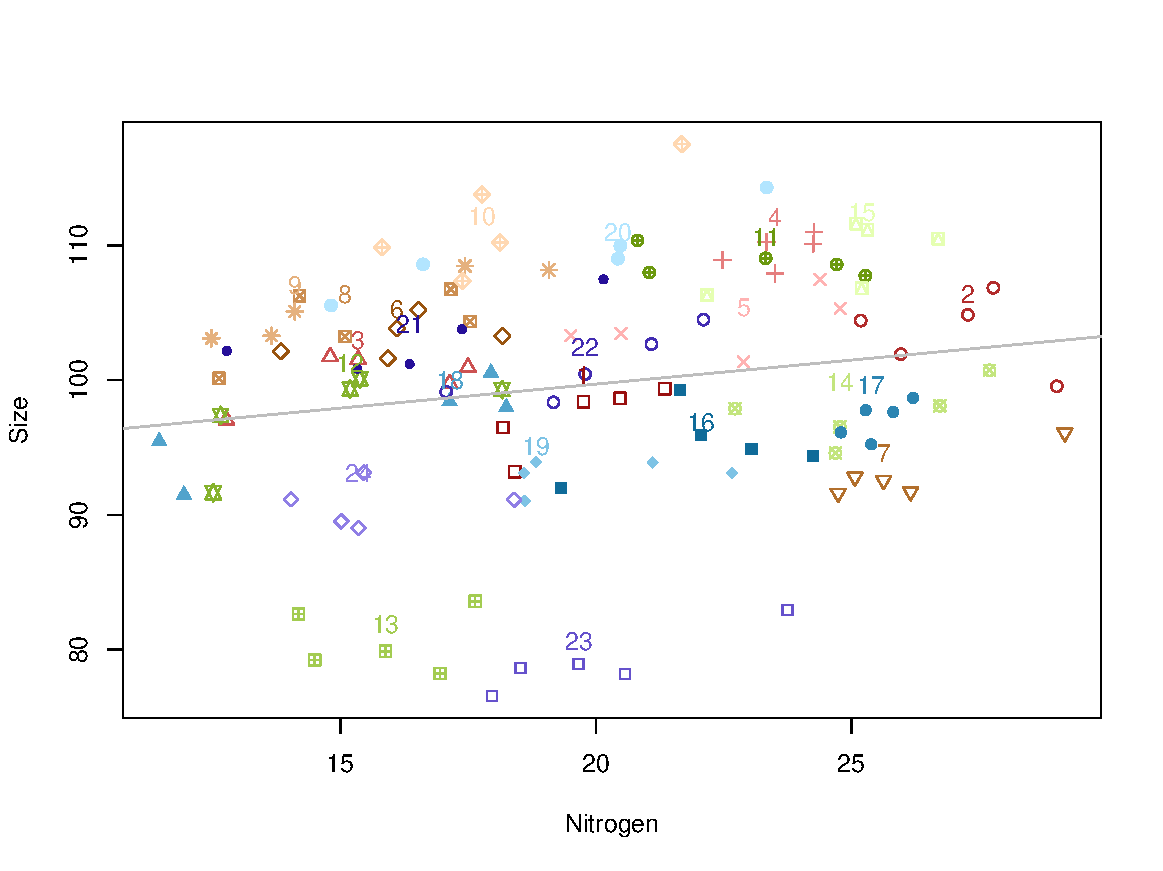
\includegraphics[scale=0.5]{Kap3/hlrm_ols_farms.pdf}
    \caption{Scatter plot of plant size against soil nitrogen concentration across 24 farms, with the global ordinary least squares fit.}
    \label{fig:hlrm_ols_farms}
\end{figure}


The results in Table~\ref{tab:goodness} highlight the trade-off between 
statistical accuracy and computational efficiency across inference methods. 
MCMC clearly outperforms both VI and SVI in terms of predictive adequacy, 
as reflected by substantially lower WAIC and DIC values, a smaller mean squared 
error (MSE), and an $R^2$ close to 1, indicating excellent fit. In contrast, 
the variational methods (VI and SVI) yield considerably poorer predictive 
performance, with WAIC and DIC values more than double those of MCMC, high MSE, 
and almost no explanatory power according to $R^2$.  

\vspace{0.5cm}

However, these improvements in accuracy come at a high computational cost: 
MCMC requires over 500 seconds of runtime, compared to roughly 55 seconds 
for both VI and SVI. This gap illustrates the typical precision–scalability 
trade-off in Bayesian computation: while MCMC provides reliable posterior 
estimates, it is less scalable to large or streaming datasets, where faster 
but approximate methods such as VI and SVI may be preferable despite their 
loss of accuracy. 

\begin{table}[ht]
\centering
\caption{Count of farm-specific $95\%$ credible intervals (CIs) containing zero for regression coefficients and variances under MCMC, VI, and SVI.}
\label{tab:ic_metodos}
\begin{tabular}{lccc}
\toprule
 & \textbf{MCMC} & \textbf{VI} & \textbf{SVI} \\
\midrule
$\beta_{1j}$   & $0/24$ & $0/24$ & $0/24$ \\
$\beta_{2j}$   & $1/24$ & $0/24$ & $0/24$ \\
$\sigma^{2}_{j}$ & $0/24$ & $0/24$ & $0/24$ \\
\bottomrule
\end{tabular}
\end{table}

\vspace{0.5cm}

Table~\ref{tab:ic_metodos} summarizes the number of credible intervals that include zero across farms for the regression coefficients and error variances. The results indicate that almost no intervals contain zero, with the only exception being $\beta_{2j}$ under MCMC in one farm. This finding is consistent with the strong signal observed in previous analyses, where nitrogen concentration showed a clear positive effect on plant size (Figure~\ref{fig:hlrm_ols_farms}) and predictive distributions concentrated around the global mean (Figure~\ref{fig:hlrm_y_density_farms}).

\begin{figure}[H]
    \centering
    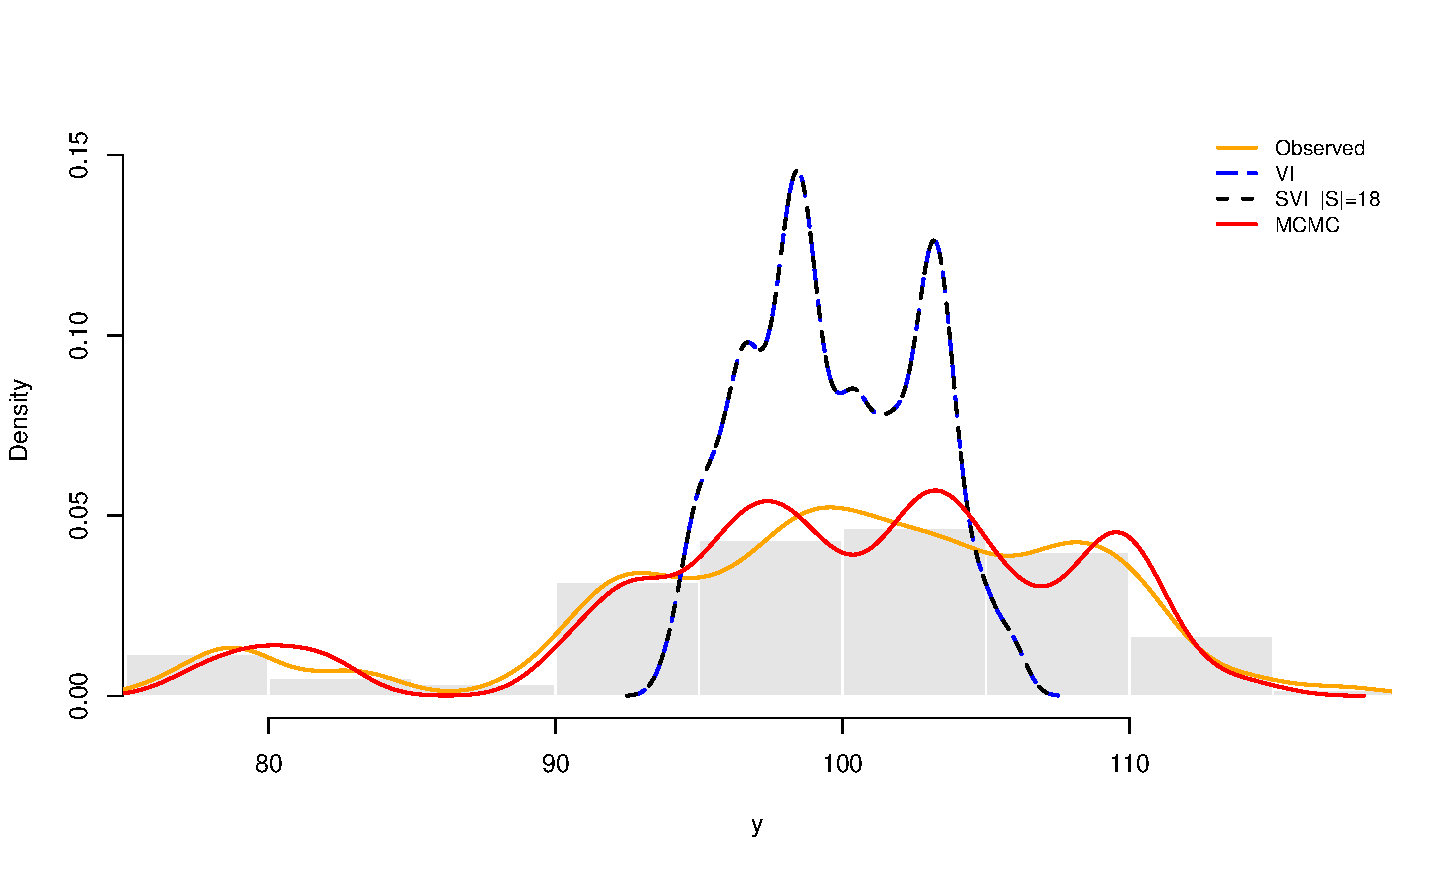
\includegraphics[scale=0.5]{Kap3/hlrm_y_density_farms.pdf}
    \caption{Posterior prediction density of plant size compared across methods.}
    \label{fig:hlrm_y_density_farms}
\end{figure}


An additional consideration is that the mean–field assumption underlying VI and SVI treats the regression coefficients and variance components as independent. This factorization simplifies computations but may overlook structural dependencies or correlations captured by MCMC. As a result, the variational methods can lose part of the joint posterior information, which may explain both the wider intervals for $\beta_{j,1}$ and the reduced sensitivity to farm-specific heterogeneity compared to MCMC.


\begin{table}[!h]
\centering
\caption{\label{tab:PPvalsHLRM}Posterior predictive $p$-values for HLRM (1000 replications), farms dataset.}
\centering
\begin{tabular}[t]{lrrrrrr}
\toprule
\textbf{Method} & \textbf{min} & \textbf{max} & \textbf{IQR} & \textbf{mean} & \textbf{median} & \textbf{sd} \\
\midrule
MCMC & 0.49 & 0.22 & 0.23 & 0.49 & 0.49 & 0.53\\
VI & 0.00 & 1.00 & 1.00 & 0.48 & 0.47 & 1.00\\
SVI & 0.00 & 1.00 & 1.00 & 0.47 & 0.46 & 1.00\\
\bottomrule
\end{tabular}
\end{table}

\newpage

Table~\ref{tab:PPvalsHLRM} reports the posterior predictive $p$-values for the hierarchical linear regression model fitted to the farms dataset. Under MCMC, the distribution of $p$-values appears well-calibrated, with values centered around 0.49 and moderate dispersion (sd = 0.53), suggesting an adequate fit that reflects both central and extreme features of the data. In contrast, both VI and SVI display degenerate behavior, with minimum and maximum values equal to 0 and 1, and an interquartile range (IQR) of 1.0. This indicates that the variational approximations are overly concentrated, yielding posterior predictive distributions that fail to capture the tails of the empirical distribution.  

\vspace{0.5cm}

The inflated posterior predictive $p$-values observed under VI and SVI are a direct consequence of the shrinkage effect introduced by the mean–field approximation. By pulling estimates toward the global mean, variational inference reduces variability and underrepresents extreme observations in the dataset. As a result, measures based on the extremes (min, max, and IQR) are poorly captured, highlighting the limitations of variational methods for fully characterizing uncertainty in hierarchical structures.

\vspace{0.5cm}

Figures~\ref{fig:hlrm_betas_pairs_farms} and \ref{fig:hlrm_sigma2j_farms} present the posterior estimates for the farm-specific intercepts, slopes, and error variances under MCMC, VI, and SVI. The most notable differences between methods appear in the intercepts $\beta_{j,1}$, where the variational approaches tend to produce wider credible intervals. In most cases, the variational intervals contain those obtained by MCMC, reflecting a conservative approximation. This pattern is consistent with the shrinkage effect observed in the predictive density results (Figure~\ref{fig:hlrm_y_density_farms}), where posterior mass accumulated around the global mean. 

\vspace{0.5cm}

Notably, the variational methods (VI and SVI) produce slightly wider intervals, as discussed earlier, but still avoid including zero, which suggests that the main direction of the effect is robust across inference methods. The difference lies in the treatment of uncertainty: while MCMC more accurately captures posterior variability, VI and SVI, due to their mean–field approximation, may underestimate potential dependencies and therefore simplify the structure of the credible intervals.

\vspace{0.5cm}

Figure~\ref{fig:hlrm_sigma2j_farms} presents the posterior means and 95\% credible intervals of the farm-specific error variances under MCMC, VI, and SVI. A systematic pattern is observed: while the posterior means of VI and SVI remain closely aligned with those of MCMC, their credible intervals are consistently wider. This inflation of uncertainty is a direct consequence of the mean–field factorization, which forces independence between regression coefficients and variance parameters, thereby discarding posterior correlations that MCMC naturally captures. As a result, the additional variability observed in VI and SVI should not be interpreted as genuine posterior uncertainty, but rather as an artifact of the variational approximation.  

\newpage

\begin{landscape}
\begin{figure}[H]
    \centering
    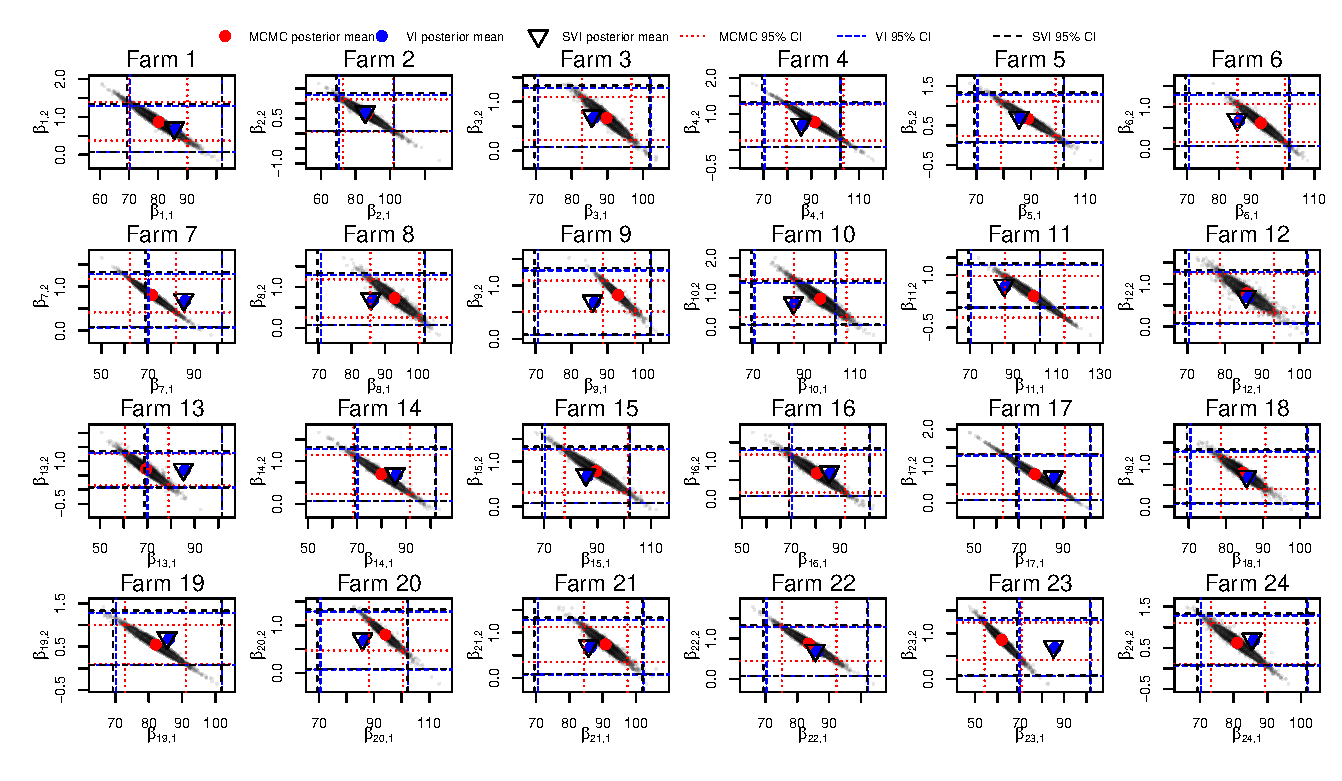
\includegraphics[scale=0.95]{Kap3/hlrm_betas_pairs_farms.pdf}
    \caption{Posterior means and 95\% credible intervals for farm-specific regression coefficients, comparing MCMC, VI, and SVI with $|S|=18$.}
    \label{fig:hlrm_betas_pairs_farms}
\end{figure}
\end{landscape}


\newpage
\begin{landscape}
\begin{figure}[H]
    \centering
    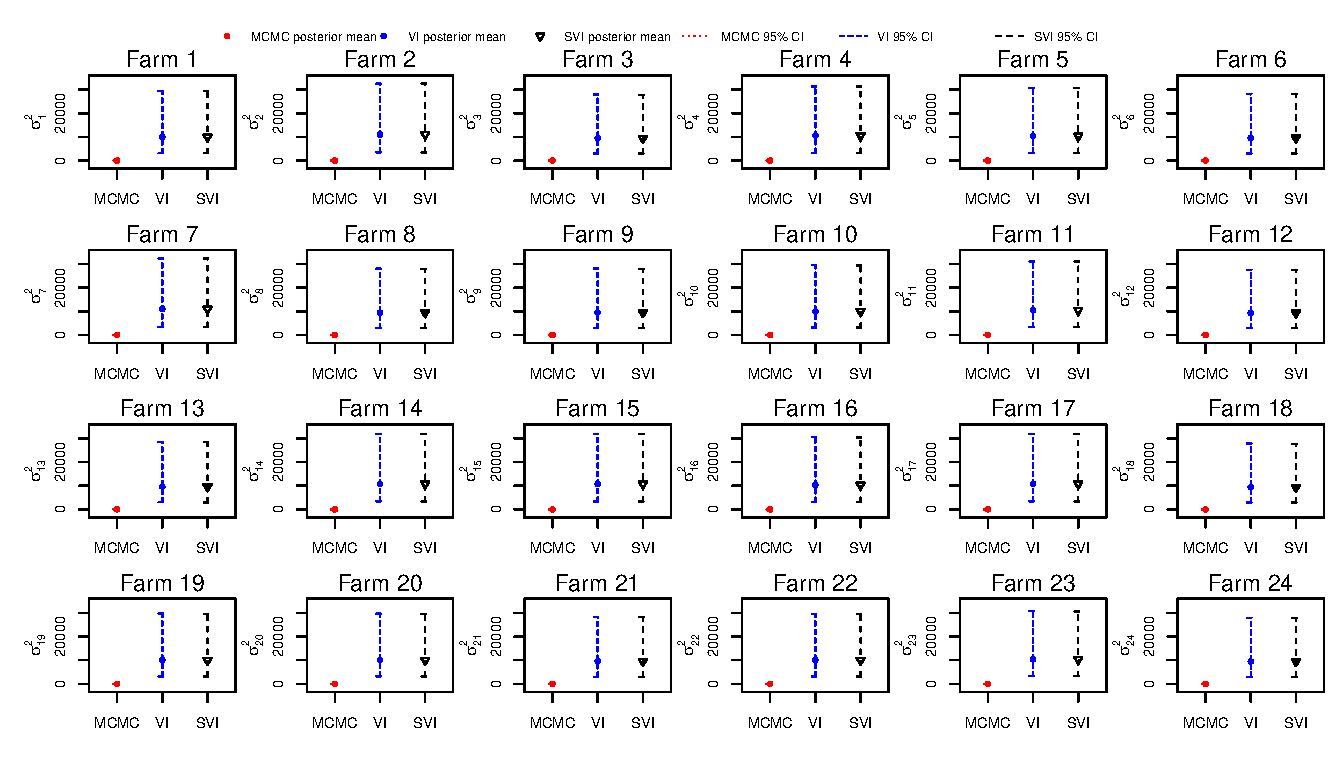
\includegraphics[scale=1]{Kap3/hlrm_sigma2j_farms.pdf}
    \caption{Posterior means and 95\% credible intervals for farm-specific error variances, comparing MCMC, VI, and SVI with $|S|=18$.}
    \label{fig:hlrm_sigma2j_farms}
\end{figure}
\end{landscape}

\begin{landscape}
\begin{figure}[H]
    \centering
    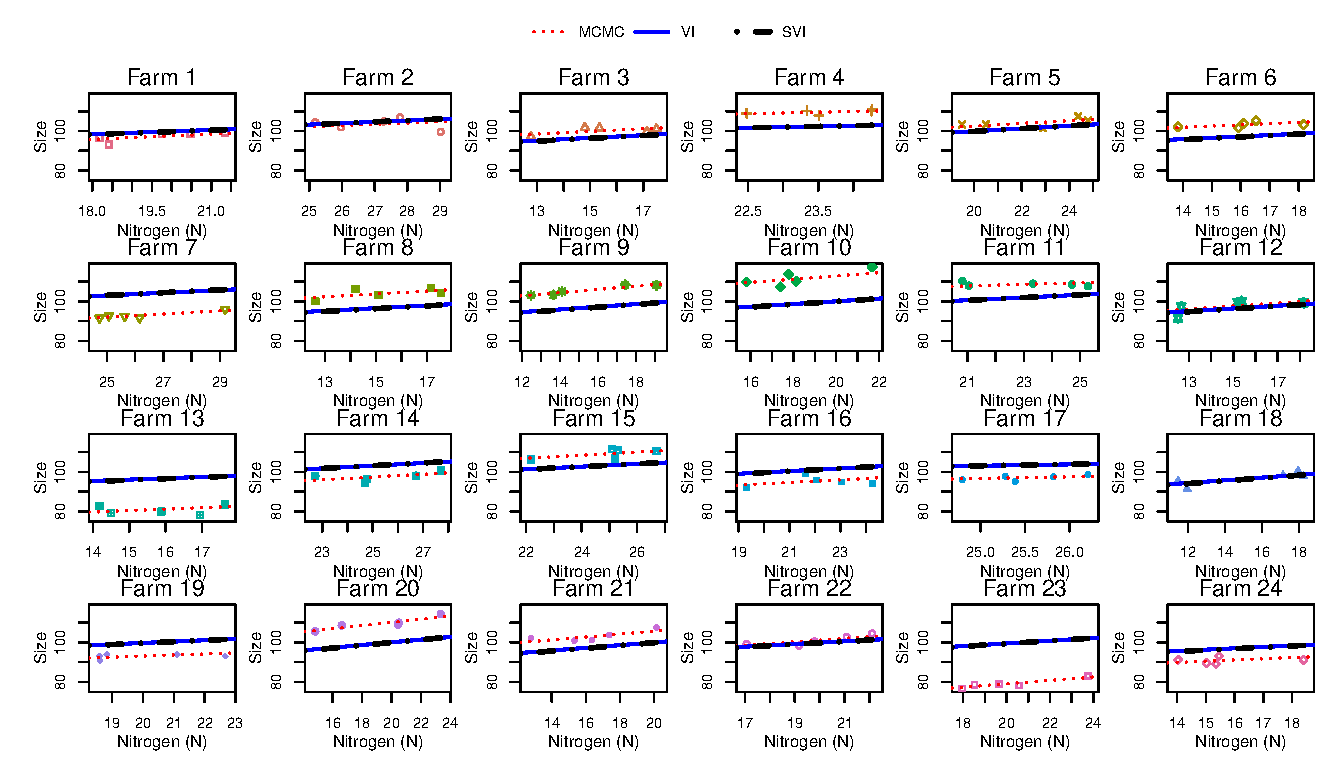
\includegraphics[scale=0.95]{Kap3/hlrm_lines_farms.pdf}
        \caption{Posterior regression lines of plant size on soil nitrogen concentration across farms, comparing MCMC, VI, and SVI with $|S|=18$.}
    \label{fig:hlrm_lines_farms}
\end{figure}
\end{landscape}

This behavior propagates into the regression lines displayed in Figure~\ref{fig:hlrm_lines_farms}. Across most farms, the three methods produce very similar fits, confirming that the dominant nitrogen effect is recovered regardless of the inference strategy. However, in some farms (e.g., 7, 10, 20, and 23), the lines obtained with SVI deviate slightly from those of MCMC and VI. These discrepancies stem from the larger credible intervals associated with the regression coefficients under SVI, which generate more dispersed predictions at the group level. Critically, this highlights a key trade-off: whereas MCMC preserves the full posterior dependence structure and provides more precise local inference, VI and SVI deliver faster approximations at the expense of overestimated variances and a loss of granularity in group-specific effects. Consequently, variational methods may suffice for global predictive purposes, but they are less reliable for fine-grained inference where local parameter dependence is essential.

\section{Clustering Hierarchical Normal Linear Regression Model}

As stated by  \cite{SOSA} an extension of Hierarchical Normal Linear Regression is use the model to capture existing but not explicit defined group structures changing the task of model the response for clustering task with the idea of generate clustering of the hierarchical levels thought as natural clusters and including all its individuals within itself in the cluster of clusters, specifyng the model like Gaussian Mixture to be able of capture this estructure mentioned before.


\vspace{0.5cm}

\cite{SOSA} propose specify the model relaxing the normal assumption representing the response as a finite Gaussian Mixture as follows:

\begin{equation}
\label{CHRLM}
y_{ij} \mid \bm{x}_{ij}, \lbrace\bm{\beta}_k\rbrace, \lbrace\sigma_k^2 \rbrace \stackrel{\text { ind }}{\sim} \sum_{k=1}^{K}\omega_k\mathsf{N}\left(y_{ij}\mid\bm{x}_{ij}^{\bm{\top}} \bm{\beta}_k, \sigma_k^2\right), \quad i=1, \ldots, n_j, \quad j=1, \ldots, m
\end{equation}

where $K$ is a positive fixed integer that represents the number of clusters, $\bm{\beta}_1\cdots\bm{\beta}_K$ and $\sigma^2_1\cdots\sigma^2_K$ are the cluster-specific regression parameters and the cluster-specific variances of the mixture, and $\omega_1,\cdots,\omega_K$ are the mixture probabilities satisfying $\sum_{k=1}^{K}\omega_k=1\text{ and }0<\omega_k<1$.

\vspace{0.5cm}

Another way of expressing the model in \ref{CHRLM} is reparametrize the model by assuming that $P(\gamma_j=k)=\omega_k\text{ for   }j=1, \ldots, m\text{ and }k=1, \ldots, K$ where $\gamma_j$ is a categorical variable that denotes the cluster assignment and takes values $k=1, \ldots, K$ with probabilities $\omega_1,\cdots,\omega_K$. So that the model in \ref{CHRLM} can be written as follows:

\begin{equation}
\label{CHRLM2}
y_{ij} \mid \bm{x}_{ij}, \gamma_j,\bm{\beta}_{\gamma_j},\sigma_{\gamma_j}^2\stackrel{\text { ind }}{\sim} \mathsf{N}\left(y_{ij}\mid\bm{x}_{ij}^{\bm{\top}} \bm{\beta}_{\gamma_j}, \sigma_{\gamma_j}^2\right), \quad i=1, \ldots, n_j, \quad j=1, \ldots, m
\end{equation}

\newpage

\subsection{Prior Distributions}

To continue with Bayesian methodology and propose the prior distributions for model in \ref{CHRLM2}, whit parameters vector $\bm{\Theta}=\left(\gamma, \bm{\omega}, \bm{\zeta}, \bm{\sigma}^2, \bm{\beta}, \bm{\Sigma}, \xi^2\right)$ where $\bm{\gamma}=\left(\gamma_1, \ldots, \gamma_m\right), \bm{\omega}=\left(\omega_1, \ldots, \omega_K\right), \bm{\zeta}=\left(\bm{\beta}_1, \ldots, \bm{\beta}_K\right), \bm{\sigma}^{\mathbf{2}}=\left(\sigma_1^2, \ldots, \sigma_K^2\right)$ represented by figure \ref{fig:DAG_CHLRM}, as follows:

\begin{equation}
    \label{hyper_CHRLM_1}
    \gamma\left|\bm{\omega} \sim \mathsf{Cat}(\bm{\omega}), \quad \bm{\beta}_k\right| \bm{\beta}, \bm{\Sigma} \stackrel{\mathsf{iid}}{\sim} \mathsf{N_p}(\bm{\beta}, \bm{\Sigma}) \quad \text { and } \quad \sigma_k^2 \mid \xi^2 \stackrel{\mathsf{iid}}{\sim} \mathsf{IG}\left(\nu_0 / 2, \nu_0 \xi^2 / 2\right)    
\end{equation}

\begin{equation}
    \label{hyper_CHRLM_2}
    \bm{\omega} \sim \mathsf{Dir}\left(\bm{\alpha}_0\right), \quad \bm{\beta} \sim \mathsf{N_p}\left(\bm{\mu}_0, \bm{\Lambda}_0\right), \quad \bm{\Sigma} \sim \mathsf{IW}\left(n_0, \mathbf{S}_0^{-1}\right), \quad \xi^2 \sim \mathsf{G}\left(a_0, b_0\right)
\end{equation}

with  $\bm{\mu}_0, \bm{\Lambda}_0, n_0, \mathbf{S}_0, \nu_0, a_0, b_0 \text { and } \bm{\alpha}_0$ the hyperparameters of model.

\begin{figure}[H]
    \centering
    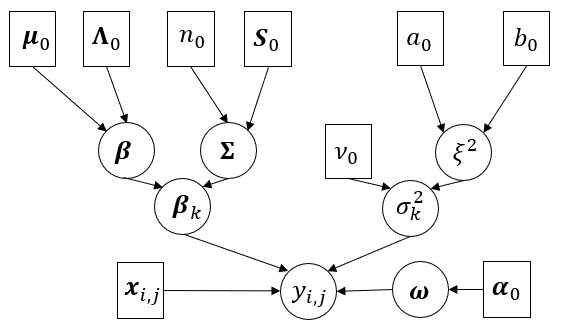
\includegraphics[scale=0.7]{Kap2/DAG_CHLRM.png}
    \caption{DAG Representation CHLRM}
    \label{fig:DAG_CHLRM}
\end{figure}

\subsubsection{Prior Elicitation}
To follow the prior elicitation strategy adopted in the previous models, we set the hyperparameters as follows. For the global regression coefficients $\bm{\beta}$, we set the prior mean as $\bm{\mu}_0 = \hat{\bm{\beta}}_{\text{OLS}}$ and the prior precision as $\bm{\Lambda}_0 = g\,\hat{\sigma}^2_{\text{OLS}}(\bm{X}^\top\bm{X})^{-1}$, where $g = \sum_{j=1}^{m} n_j$ is the total sample size. For the covariance matrix $\bm{\Sigma}$ of the cluster-level effects, we use an Inverse Wishart prior with degrees of freedom $n_0 = p + 2$ and scale matrix $\bm{S}_0 = \bm{\Lambda}_0$, inducing shrinkage consistent with the prior for $\bm{\beta}$. Each cluster-specific variance $\sigma_k^2$ is given an Inverse Gamma prior with shape $\nu_0 = 1$ and scale depending on $\xi^2$, which itself follows a Gamma prior with hyperparameters $a_0 = 1$ and $b_0 = 1/\hat{\sigma}^2_{\text{OLS}}$, allowing control over the overall variance level. Finally, the mixture weights $\bm{\omega}$ follow a Dirichlet prior with concentration parameters $\bm{\alpha}_0 = (1/K, \dots, 1/K)$, resulting in a diffuse prior that does not favor any particular cluster a priori.

\newpage

\subsection{Posterior Inference}

\subsubsection{Gibbs Sampling}

In the CHLRM framework, posterior inference will be conducted via Gibbs sampling. This allows for a straightforward sequential updating of group allocations, mixture proportions, cluster-specific parameters, and global-level variables, ultimately producing approximate samples from the joint posterior distribution, given by:

\begin{equation}
    \label{POST_CHLRM}
    \begin{split}
    p(\bm{\Theta} \mid\bm{y}, \bm{X}) 
&\propto p(\bm{y} \mid \bm{X}, \bm{\gamma}, \bm{\zeta}, \bm{\sigma}^2) 
\, p(\bm{\gamma} \mid \bm{\omega}) 
\, p(\bm{\omega}) 
\, p(\bm{\xi} \mid\bm{\beta},\bm{\Sigma}) \, p(\bm{\beta}) 
p(\bm{\Sigma}) 
\, p(\bm{\sigma}^2 \mid \xi^2) 
\, p(\xi^2)\\
&\propto \prod_{k=1}^{K}\prod_{j=1}^{m} \prod_{i=1}^{n_j} \mathsf{N}(y_{ij}\mid\bm{x}_{ij}^\top \bm{\beta}_{\gamma_j},\sigma_{\gamma_j}^2)^{[\gamma_j = k]}\times\prod_{j=1}^{m}\mathsf{Cat}(\gamma_j\mid\bm{\omega})\times\mathsf{Dir}(\bm{\omega}\mid\bm{\alpha}_0)\\
&\quad\times\prod_{k=1}^{K}\mathsf{N_p}(\bm{\beta}_k\mid\bm{\beta}, \bm{\Sigma})\times\mathsf{N_p}\left(\bm{\beta}\mid\bm{\mu}_0, \bm{\Lambda}_0\right)\times\mathsf{IW}\left(\bm{\Sigma}\mid n_0, \mathbf{S}_0^{-1}\right)\\
&\quad\times\prod_{k=1}^{K}\mathsf{IG}\left(\sigma_k^2 \mid\nu_0 / 2, \nu_0 \xi^2 / 2\right)\times\mathsf{G}\left(\xi^2 \mid a_0, b_0\right)\\
&\propto \prod_{j=1}^{m} \prod_{i=1}^{n_j} (\sigma_{\gamma_j}^2)^{-1/2} 
\exp\left\{ -\frac{1}{2\sigma_{\gamma_j}^2} (y_{ij} - \bm{x}_{ij}^\top \bm{\beta}_{\gamma_j})^2 \right\}  \times\prod_{j=1}^{m} \prod_{k=1}^{K} \omega_k ^{[\gamma_j = k]}\times\prod_{k=1}^{K}\omega_k^{\alpha_{0k}-1}\\
&\quad \times \prod_{j=1}^{m} |\bm{\Sigma}|^{-1/2} 
\exp\left\{ -\frac{1}{2} (\bm{\beta}_j - \bm{\beta})^\top \bm{\Sigma}^{-1} (\bm{\beta}_j - \bm{\beta}) \right\}  \times \prod_{k=1}^{K} |\bm{\Sigma}|^{-1/2} 
\exp\left\{ -\frac{1}{2} (\bm{\beta}_k - \bm{\mu}_0)^\top \bm{\Sigma}^{-1} (\bm{\beta}_k - \bm{\mu}_0) \right\} \\
&\quad \times |\bm{\Sigma}|^{-(n_0 + p + 1)/2} 
\exp\left\{ -\frac{1}{2} \operatorname{tr}(\bm{S}_0 \bm{\Sigma}^{-1}) \right\}  \times \prod_{j=1}^{m} (\sigma_j^2)^{-\left(\nu_0 / 2 + 1\right)} 
\exp\left\{ -\frac{\nu_0 \xi^2}{2\sigma_j^2} \right\} \times \prod_{j=1}^{m} (\xi^2)^{a_0 - 1} 
\exp\left\{ -b_0 \xi^2 \right\}
\end{split}
\end{equation}

then, the f.c.d.s for this model are:

\begin{itemize}
    \item f.c.d of $\gamma_j$ for $j=1,\cdots,m$.
    
    \begin{equation}
        \label{CHLRM_MCMC_gammaj}
        \gamma_j\mid \text{rest}\sim \mathsf{Cat}\left(\left\lbrace p(\gamma_j = 1 \mid \text{rest}),\dots,p(\gamma_j = K \mid \text{rest}\right) \rbrace\right)
    \end{equation}

    with $p(\gamma_j = k \mid \text{rest}) \propto \omega_k \prod_{i=1}^{n_j} (\sigma_k^2)^{-1/2} 
\exp\left\{ -\frac{1}{2\sigma_k^2} (y_{ij} - \bm{x}_{ij}^\top \bm{\beta}_k)^2 \right\}$

    \item f.c.d of $\bm{\omega}$

    \begin{equation}
    \label{CHLRM_MCMC_Omega}
    \bm{\omega} \mid \text{rest} \sim \mathsf{Dir}(\alpha_{01} + n_1,\,  \dots,\, \alpha_{0K} + n_K)\\
    \end{equation}

with $n_k=\#\left\lbrace j : \gamma_j=k\right\rbrace$

\item f.c.d of $\bm{\beta}_k$ for $k=1,\cdots,K$

\begin{equation}
\label{CHLRM_MCMC_Betak}
\bm{\beta}_k \mid \text{rest} \sim \mathsf{N_p}\left((\sigma_k^{-2}\bm{X}_{k}^\top\bm{X}_{k}+\bm{\Sigma}^{-1})^{-1}(\sigma_k^{-2}\bm{X}_{k}^\top\bm{y}_{k}+\bm{\Sigma}^{-1}\bm{\beta}) , (\sigma_k^{-2}\bm{X}_{k}^\top\bm{X}_{k}+\bm{\Sigma}^{-1})^{-1}\right)
\end{equation}

note that if cluster $k$ is empty, then the f.c.d of $\bm{\beta}_k$ is just $\bm{\beta}_k \mid \text{rest} \sim \mathsf{N_p}(\bm{\beta}, \bm{\Sigma})$, with $\bm{X}_{k} = [\bm{X}_j^\top : \gamma_j = k]^\top$ , where $\bm{X}_j = \left[\bm{x}_{1, j}, \ldots, \bm{x}_{n_j, j}\right]^\top$ a $n_j \times p$ matrix and $\bm{x}_{ij}$ is a $p \times 1$ vector of regressors for observation $i$ in group $j$ and $\bm{y}_{k} = [\bm{y}_j^\top : \gamma_j = k]^\top$ where $\bm{y}_j = \left[y_{1, j}, \ldots, y_{n_j, j}\right]^\top$  is a $n_j \times 1$ vector of response variable values for group $j$.

\item f.c.d of $\sigma_k^2$ for $k=1,\cdots,K$

\begin{equation}
\label{CHLRM_MCMC_sigma2k}
\sigma_k^2 \mid \text{rest} \sim\mathsf{IG} \left( 
\frac{\nu_0 + \sum_{\left\lbrace j : \gamma_j = k\right\rbrace}n_j}{2},\ 
\frac{ \nu_0 \xi^2 + (\bm{y}_{k} - \bm{X}_{k} \bm{\beta}_k)^\top(\bm{y}_{k} - \bm{X}_{k} \bm{\beta}_k) }{2} 
\right)
\end{equation}

note that if cluster $k$ is empty, then the f.c.d of $\sigma_k^2$ is just $\sigma_k^2 \mid \text{rest} \sim\mathsf{IG}\left(\frac{\nu_0}{2},\frac{ \nu_0 \xi^2}{2}\right) $.

\item f.c.d of $\xi^2$

\begin{equation}
\label{CHLRM_MCMC_xi2}
\xi^2 \mid \text{rest} \sim \mathsf{G} \left(
\frac{\kappa \nu_0}{2} + a_0,\ 
\frac{\nu_0}{2} \sum_{\left\lbrace k : n_k > 0\right\rbrace} \sigma_k^{-2} + b_0
\right)
\end{equation}

where $\kappa = \#\left\lbrace k : n_k > 0\right\rbrace$ is the number of non empty clusters.

\item f.c.d of $\bm{\beta}$

\begin{equation}
\label{CHLRM_MCMC_Beta}
\bm{\beta} \mid \text{rest} \sim  \mathsf{N_p}\left(\left( \kappa \bm{\Sigma}^{-1} + \bm{\Lambda}_0^{-1} \right)^{-1}\left( \bm{\Lambda}_0^{-1} \bm{\mu}_0 + \bm{\Sigma}^{-1} \sum_{\left\lbrace k : n_k > 0\right\rbrace} \bm{\beta}_k \right), \left( \kappa \bm{\Sigma}^{-1} + \bm{\Lambda}_0^{-1} \right)^{-1}\right)
\end{equation}

\item f.c.d of $\bm{\Sigma}$

\begin{equation}
\label{CHLRM_MCMC_Sigma}
\bm{\Sigma} \mid \text{rest} \sim \mathsf{IW} \left(
\kappa + n_0,\ 
\left(\bm{S}_0 + \sum_{\left\lbrace k : n_k > 0\right\rbrace} (\bm{\beta}_k - \bm{\beta})(\bm{\beta}_k - \bm{\beta})^\top
\right)^{-1}\right)
\end{equation}


\end{itemize}

\begin{algorithm}[H]
\caption{Gibbs Sampling for CHLRM}
\begin{algorithmic}
\State \textbf{Input} Initial values $\{\gamma_j^{(0)}\}_{j=1}^m$, $\bm{\omega}^{(0)}$, $\{\bm{\beta}_k^{(0)}\}_{k=1}^K$, $\bm{\beta}^{(0)}$, $\bm{\Sigma}^{(0)}$, $\{(\sigma_k^2)^{(0)}\}_{k=1}^K$, $\xi^{2(0)}$, hyperparameters $\bm{\mu}_0, \bm{\Lambda}_0, n_0, \bm{S}_0, a_0, b_0, \nu_0$, data values $\{\bm{y}_j,\bm{X}_j\}_{j=1}^m$
\For{$b = 1, \dots, B$}
  \For{$j = 1, \dots, m$}
    \State Sample $\gamma_j^{(b)} \sim p\!\left(\gamma_j \mid \bm{\omega}^{(b-1)}, \{\bm{\beta}_k^{(b-1)}, (\sigma_k^2)^{(b-1)}\}_{k=1}^K, \bm{y}_j, \bm{X}_j \right)$ from eq.\ref{CHLRM_MCMC_gammaj}
  \EndFor
  \State Sample $\bm{\omega}^{(b)} \sim p\!\left(\bm{\omega} \mid \{\gamma_j^{(b)}\}_{j=1}^m \right)$ from eq.~\ref{CHLRM_MCMC_Omega}
  \For{$k = 1, \dots, K$}
    \State Sample $\bm{\beta}_k^{(b)} \sim p\!\left(\bm{\beta}_k \mid \bm{\beta}^{(b-1)}, \bm{\Sigma}^{(b-1)}, (\sigma_k^2)^{(b-1)}, \{\bm{y}_j, \bm{X}_j, \gamma_j^{(b)}\}_{j=1}^m \right)$ from eq.~\ref{CHLRM_MCMC_Betak}
    \State Sample $(\sigma_k^2)^{(b)} \sim p\!\left(\sigma_k^2 \mid \bm{\beta}_k^{(b)}, (\xi^2)^{(b-1)}, \{\bm{y}_j, \bm{X}_j, \gamma_j^{(b)}\}_{j=1}^m \right)$ from eq.~\ref{CHLRM_MCMC_sigma2k}
  \EndFor
  \State Sample $\bm{\beta}^{(b)} \sim p\!\left(\bm{\beta} \mid \{\bm{\beta}_k^{(b)}\}_{k=1}^K, \bm{\Sigma}^{(b-1)} \right)$ from eq.~\ref{CHLRM_MCMC_Beta}
  \State Sample $\bm{\Sigma}^{(b)} \sim p\!\left(\bm{\Sigma} \mid \{\bm{\beta}_k^{(b)}\}_{k=1}^K, \bm{\beta}^{(b)} \right)$ from eq.~\ref{CHLRM_MCMC_Sigma}
  \State Sample $(\xi^2)^{(b)} \sim p\!\left(\xi^2 \mid \{(\sigma_k^2)^{(b)}\}_{k=1}^K \right)$ from eq.~\ref{CHLRM_MCMC_xi2}
\EndFor
\State \textbf{Output} Draws $\{\gamma_j^{(b)},\bm{\omega}^{(b)},\bm{\beta}_k^{(b)},(\sigma_k^2)^{(b)},\bm{\beta}^{(b)},\bm{\Sigma}^{(b)},(\xi^2)^{(b)}\}_{b=1}^B$
\end{algorithmic}
\end{algorithm}


For detailed and explicit derivations of these results, see Appendix \ref{Appendix_B}.

\subsubsection{CAVI}

As before, we specify a variational distribution to approximate the posterior distribution under the mean--field assumption described in result \ref{MFA}. Leveraging the CAVI framework for conditionally conjugate models presented in \ref{NMVFB_opt}, we derive the update rules for each variational factor in the CHLRM. It is important to highlight that these variational factors naturally decompose into local parameters, which are specific to each group assignment variable and its associated cluster-level effects, and global parameters, which correspond to latent variables shared across all clusters.

\begin{equation}
\label{Q_CHLRM}
\begin{split}
q(\bm{\Theta})&=\prod_{k=1}^{K}q(\bm{\beta}_k)q(\bm{\beta})q(\bm{\Sigma})\prod_{k=1}^{K}q(\sigma_k^2)q(\xi^2)\prod_{j=1}^{m}q(\gamma_j)q(\bm{\omega})\\
&= \left(q(\bm{\omega})q(\bm{\beta})q(\bm{\Sigma})q(\xi^2)\prod_{k=1}^{K}q(\bm{\beta}_k)q(\sigma_k^2)\right)\left(\prod_{j=1}^{m}q(\gamma_j)\right)
\end{split}
\end{equation}

\begin{itemize}
    \item Factor  $q(\gamma_j)=\mathsf{Cat}(\lbrace{\rho_{j1},\dots,\rho_{jK}\rbrace})$, with

\begin{equation}
\label{CHLRM_CAVI_rhojk_gamma}
\log \rho_{jk} \propto -\tfrac{n_j}{2}\mathsf{E}_{\sigma^2_k}\left[\log\sigma^2_{k}\right]
-\tfrac{1}{2}\mathsf{E}_{\sigma^2_k}\left[\frac{1}{\sigma^2_{k}}\right]\mathsf{E}_{\bm{\beta}_k}\left[\left(\bm{y}_{j}-\bm{X}_{j}\bm{\beta}_{k}\right)^\top\left(\bm{y}_{j}-\bm{X}_{j}\bm{\beta}_{k}\right)\right]+\mathsf{E}_{\omega}\left[\log\omega_k\right]
\end{equation}

\item Factor $q(\bm{\omega})=\mathsf{Dir}\left(\left\lbrace \alpha_{\bm{\omega}1},\dots,\alpha_{\bm{\omega}K}\right\rbrace\right)$, with

\begin{equation}
    \label{CHLRM_CAVI_Alpha_Omega}
    \alpha_{\bm{\omega}k}=\alpha_{0k}+\sum_{j=1}^{m}\mathsf{E}_{\gamma_j}\left[[\gamma_j=k]\right]
\end{equation}

\item Factor $q(\bm{\beta}_k)=\mathsf{N_p}(\bm{\mu}_{\bm{\beta}_k},\bm{\Sigma}_{\bm{\beta}_k})$, with

\begin{equation}
\label{CHLRM_CAVI_Sigma_Betak}
\bm{\Sigma}_{\bm{\beta}_k}^{-1} = \mathsf{E}_{\sigma^2_k}\left[{\sigma_k}^{-2}\right] \sum_{j=1}^{m}\mathsf{E}_{\gamma_j}\left[[\gamma_j=k\right]]\bm{X}_{j}^\top \bm{X}_{j}  + \mathsf{E}_{\bm{\Sigma}}\left[\bm{\Sigma}^{-1}\right] ,
\end{equation}

\begin{equation}
\label{CHLRM_CAVI_Mu_Betak}
\bm{\mu}_{\bm{\beta}_k}= \bm{\Sigma}_{\bm{\beta}_k}\left[\mathsf{E}_{\sigma^2_k}\left[{\sigma_k}^{-2}\right] \sum_{j=1}^{m}\mathsf{E}_{\gamma_j}\left[[\gamma_j=k\right]]\bm{X}_{j}^\top \bm{y}_{j} + \mathsf{E}_{\bm{\Sigma}}\left[\bm{\Sigma}^{-1}\right] \mathsf{E}_{\bm{\beta}}\left[\bm{\beta} \right] \right]
\end{equation}

\item Factor $q(\bm{\beta})=\mathsf{N_p}(\bm{\mu}_{\bm{\beta}},\bm{\Sigma}_{\bm{\beta}})$, with

\begin{equation}
\label{CHLRM_CAVI_Sigma_Beta}
\bm{\Sigma}_{\bm{\beta}} = \left[\bm{\Lambda}_0^{-1}   + \sum_{k=1}^{K}\mathsf{E}_{\bm{\Sigma}}\left[\bm{\Sigma}^{-1}\right]  \right] ^{-1},
\end{equation}

\begin{equation}
\label{CHLRM_CAVI_Mu_Beta}
\bm{\mu}_{\bm{\beta}}= \left[\bm{\Lambda}_0^{-1}   + \sum_{k=1}^{K}\mathsf{E}_{\bm{\Sigma}}\left[\bm{\Sigma}^{-1}\right]  \right]^{-1}\left[\bm{\Lambda}_0^{-1} \bm{\mu}_0 + \sum_{k=1}^{K}\mathsf{E}_{\bm{\Sigma}}\left[\bm{\Sigma}^{-1}\right] \mathsf{E}_{\bm{\beta}_k}\left[\bm{\beta}_k \right]\right]
\end{equation}

\item Factor $q(\bm{\Sigma})=\mathsf{IW}(\nu_{\bm{\Sigma}},\bm{S}_{\bm{\Sigma}}^{-1})$, with

\begin{equation}
\label{CHLRM_CAVI_nu_Sigma}
\nu_{\bm{\Sigma}} = n_0+K,
\end{equation}

\begin{equation}
\label{CHLRM_CAVI_S_Sigma}
\bm{S}_{\bm{\Sigma}}=  \bm{S}_0 + \sum_{k=1}^{K} \mathsf{E}_{\bm{\beta}_k,\bm{\beta}}\left[\left(\bm{\beta}_k - \bm{\beta})(\bm{\beta}_k - \bm{\beta}\right)^\top\right]
\end{equation}

\item Factor $q(\sigma_k^2)=\mathsf{IG}(a_{\sigma_k^2},b_{\sigma_k^2})$, with

\begin{equation}
\label{CHLRM_CAVI_a_sigma2k}
a_{\sigma_k^2}= \frac{\nu_0 + \sum_{j=1}^{m}\mathsf{E}_{\gamma_j}\left[[\gamma_j=k]\right]n_j}{2},
\end{equation}

\begin{equation}
\label{CHLRM_CAVI_b_sigma2k}
b_{\sigma_k^2}= \frac{ \nu_0 \mathsf{E}_{\xi^2}\left[\xi^2\right] +  \sum_{j=1}^{m}\mathsf{E}_{\gamma_j}\left[[\gamma_j=k]\right]\mathsf{E}_{\bm{\beta}_k}\left[\left(\bm{y}_{j} - \bm{X}_{j} \bm{\beta}_k)^\top(\bm{y}_{j} - \bm{X}_{j} \bm{\beta}_k\right)\right]}{2}
\end{equation}

\item Factor $q(\xi^2)=\mathsf{G}(a_{\xi^2},b_{\sigma_j^2})$, with

\begin{equation}
\label{CHLRM_CAVI_a_xi2}
a_{\xi^2}=  a_0 +\sum_{k=1}^{K}\frac{\nu_0}{2},
\end{equation}

\begin{equation}
\label{CHLRM_CAVI_b_xi2}
b_{\xi^2}= b_0 + \frac{\nu_0}{2} \sum_{k=1}^{K} \mathsf{E}_{\sigma^2_k}\left[\sigma_k^{-2}\right]
\end{equation}

\item ELBO $\mathcal{L}(q(\bm{\Theta}))$

\begin{equation}
\label{CHLRM_CAVI_ELBO}
\begin{split}
\mathcal{L}(q(\bm{\Theta}))
&=\mathsf{E}_{\bm{\Theta}}\left[\log p(\bm{\Theta},\bm{y}, \bm{X})\right]-\mathsf{E}_{\bm{\Theta}}\left[\log q(\bm{\Theta})\right]\\
&= \mathsf{E}_{\bm{\Theta}}\left[\log p(\bm{y}\mid\bm{X},\bm{\gamma},\bm{\zeta},\bm{\sigma}^2)\right] + \sum_{j=1}^{m}\left(\mathsf{E}_{\bm{\Theta}}\left[\log p(\gamma_j\mid\bm{\omega})\right] -\mathsf{E}_{\gamma_j}\left[\log q(\gamma_j)\right]\right) \\
&\quad + \left(\mathsf{E}_{\bm{\Theta}}\left[\log p(\bm{\omega})\right]- \mathsf{E}_{\bm{\omega}}\left[\log q(\bm{\omega})\right]\right)+ \sum_{k=1}^{K}\left(\mathsf{E}_{\bm{\Theta}}\left[\log p(\bm{\beta}_k\mid\bm{\beta},\bm{\Sigma})\right] -\mathsf{E}_{\bm{\beta}_k}\left[\log q(\bm{\beta}_k)\right]\right)\\
&\quad + \left(\mathsf{E}_{\bm{\Theta}}\left[\log p(\bm{\beta})\right]- \mathsf{E}_{\bm{\beta}}\left[\log q(\bm{\beta})\right]\right) + \left(\mathsf{E}_{\bm{\Theta}}\left[\log p(\bm{\Sigma})\right]-\mathsf{E}_{\bm{\Sigma}}\left[\log q(\bm{\Sigma})\right] \right)\\
&\quad + \sum_{k=1}^{K}\left(\mathsf{E}_{\bm{\Theta}}\left[\log p(\sigma_k^2 \mid \xi^2)\right]-\mathsf{E}_{\sigma_k^2}\!\left[\log q(\sigma_k^2)\right]\right) + \left(\mathsf{E}_{\bm{\Theta}}\left[\log p(\xi^2)\right]- \mathsf{E}_{\xi^2}\!\left[\log q(\xi^2)\right]\right) 
\end{split}
\end{equation}

where

\begin{itemize}
    \item 
    $
    \begin{aligned}
       \mathsf{E}_{\bm{\Theta}}\left[\log p(\bm{y}\mid\bm{X},\bm{\gamma},\bm{\zeta},\bm{\sigma}^2)\right]&=\sum_{j=1}^{m}\sum_{k=1}^{K}\Bigg[\rho_{jk}\Bigg(
-\tfrac{n_j}{2}\log(2\pi)
-\tfrac{n_j}{2}\left(\log b_{\sigma_k^2}-\psi(a_{\sigma_k^2})\right) \\
&\qquad
-\tfrac{1}{2}\left(\tfrac{a_{\sigma_k^2}}{b_{\sigma_k^2}}\right)
\Big[
(\bm{y}_j-\mathbf{X}_j\bm{\mu}_{\bm{\beta}_k})^\top(\bm{y}_j-\mathbf{X}_j\bm{\mu}_{\bm{\beta}_k})
+\operatorname{tr}\left(\mathbf{X}_j^\top\mathbf{X}_j\,\bm{\Sigma}_{\bm{\beta}_k}\right)
\Big]
\Bigg)\Bigg] \\ 
    \end{aligned}
    $

    \item 
    $
    \mathsf{E}_{\bm{\Theta}}\left[\log p(\gamma_j\mid\bm{\omega})\right]=\sum_{k=1}^{K}\rho_{jk}
\Bigg[
\psi\left(\alpha_{0k}+\sum_{j=1}^{m}\rho_{jk}\right) -\psi\left(\sum_{k=1}^{K}\left[\alpha_{0k}+\sum_{j=1}^{m}\rho_{jk} \right]\right)
\Bigg]
    $

    \item 
    $
      \mathsf{E}_{\gamma_j}\left[\log q(\gamma_j)\right]=\sum_{k=1}^{K}\rho_{jk}\log\rho_{jk}  
    $

    \item 
    $
        \mathsf{E}_{\bm{\Theta}}\left[\log p(\bm{\omega})\right]=\log\Gamma\left( \sum_{k=1}^{K} \alpha_{0k} \right)-\sum_{k=1}^{K} \log\Gamma\left(\alpha_{0k}\right)+\sum_{k=1}^{K}\left(\alpha_{0k}-1\right)\left[\psi\left(\alpha_{0k}\right) -\psi\left(\sum_{k=1}^{K}\alpha_{0k}\right)\right] 
    $

        \item 
    $
    \begin{aligned}
    \mathsf{E}_{\bm{\omega}}\left[\log q(\bm{\omega})\right]
    &=\log\Gamma\left( \sum_{k=1}^{K} \left[\alpha_{0k}+\sum_{j=1}^{m}\rho_{jk} \right]\right)-\sum_{k=1}^{K} \log\Gamma\left(\alpha_{0k}+\sum_{j=1}^{m}\rho_{jk}\right)\\
        &\quad+\sum_{k=1}^{K}\left(\alpha_{0k}+\sum_{j=1}^{m}\rho_{jk} -1\right)\left[\psi\left(\alpha_{0k}+\sum_{j=1}^{m}\rho_{jk}\right) -\psi\left(\sum_{k=1}^{K}\left[\alpha_{0k}+\sum_{j=1}^{m}\rho_{jk} \right]\right)\right]
    \end{aligned}
    $

        \item

    $
        \begin{aligned}
        \mathsf{E}_{\bm{\Theta}}\left[\log p(\bm{\beta}_k\mid\bm{\beta},\bm{\Sigma})\right]=&
    -\tfrac{p}{2}\log(2\pi)
    -\tfrac{1}{2}\Bigg(
    -\sum_{i=1}^{p}\psi\!\!\left(\tfrac{\nu_{\bm{\Sigma}}+1-i}{2}\right)-p\log 2+\log|\bm{S}_{\bm{\Sigma}}^{-1}|
    \Bigg) \\
    &\qquad
    -\tfrac{1}{2}\operatorname{tr}\left(\bm{S}_{\bm{\Sigma}}^{-1}\!\!\left[
    (\bm{\mu}_{\bm{\beta}_k}-\bm{\mu}_{\bm{\beta}})
    (\bm{\mu}_{\bm{\beta}_k}-\bm{\mu}_{\bm{\beta}})^\top
    +\bm{\Sigma}_{\bm{\beta}_k}+\bm{\Sigma}_{\bm{\beta}}
    \right]\right)\\
        \end{aligned}
    $

        \item

    $
    \mathsf{E}_{\bm{\beta}_k}\left[\log q(\bm{\beta}_k)\right]=-\tfrac{p}{2}\log(2\pi e)-\tfrac{1}{2}\log|\bm{\Sigma}_{\bm{\beta}_k}|
    $

        \item 

    $
    \begin{aligned}
        \mathsf{E}_{\bm{\Theta}}\left[\log p(\bm{\beta})\right]=-\tfrac{p}{2}\log(2\pi)-\tfrac{1}{2}\log|\bm{\Lambda}_0|
-\tfrac{1}{2}\Big[
(\bm{\mu}_{\bm{\beta}}-\bm{\mu}_0)^\top\bm{\Lambda}_0^{-1}(\bm{\mu}_{\bm{\beta}}-\bm{\mu}_0)
+\operatorname{tr}\!\!\left(\bm{\Lambda}_0^{-1}\bm{\Sigma}_{\bm{\beta}}\right)
\Big]
    \end{aligned}
    $

        \item 

    $
    \begin{aligned}
        \mathsf{E}_{\bm{\beta}}\left[\log q(\bm{\beta})\right]=-\tfrac{p}{2}\log(2\pi e)-\tfrac{1}{2}\log|\bm{\Sigma}_{\bm{\beta}}|
    \end{aligned}
    $

            \item 

    $
    \begin{aligned}
\mathsf{E}_{\bm{\Theta}}\left[\log p(\bm{\Sigma})\right] &=
\tfrac{n_0}{2}\log|\bm{S}_0|-\tfrac{n_0 p}{2}\log 2-\log\Gamma_p\!\!\left(\tfrac{n_0}{2}\right)
-\tfrac{n_0+p+1}{2}\Bigg(
-\sum_{i=1}^{p}\psi\!\!\left(\tfrac{\nu_{\bm{\Sigma}}+1-i}{2}\right)-p\log 2+\log|\bm{S}_{\bm{\Sigma}}^{-1}|
\Bigg) \\
&\qquad
-\tfrac{\nu_{\bm{\Sigma}}}{2}\operatorname{tr}\left(\bm{S}_0\,\bm{S}_{\bm{\Sigma}}^{-1}\right)
    \end{aligned}
    $

        \item 

    $
    \begin{aligned}
        \mathsf{E}_{\bm{\Sigma}}\left[\log q(\bm{\Sigma})\right]&=\tfrac{\nu_{\bm{\Sigma}}}{2}\log|\mathbf{S}_{\bm{\Sigma}}|
- \tfrac{\nu_{\bm{\Sigma}} p}{2}\log 2
- \log\Gamma_p\left(\tfrac{\nu_{\bm{\Sigma}}}{2}\right) - \tfrac{\nu_{\bm{\Sigma}}+p+1}{2}\left(
-\sum_{i=1}^{p}\psi\left(\tfrac{\nu_{\bm{\Sigma}}+1-i}{2}\right)-p\log 2+\log|\mathbf{S}_{\bm{\Sigma}}^{-1}|
\right) \\ 
&\quad - \tfrac{\nu_{\bm{\Sigma}}}{2}\operatorname{tr}\left(\mathbf{S}_{\bm{\Sigma}}^2\right)
    \end{aligned}
    $

            \item 

    $
    \begin{aligned}
    \mathsf{E}_{\bm{\Theta}}\left[\log p(\bm{\sigma}_k^2 \mid \xi^2)\right]&=\tfrac{\nu_0}{2}\log\left(\tfrac{\nu_0}{2}\right)
+\tfrac{\nu_0}{2}\left(\psi(a_{\xi^2})-\log b_{\xi^2}\right)-\log\Gamma\left(\tfrac{\nu_0}{2}\right)-\tfrac{\nu_0\sigma^2_0}{2}\left(\tfrac{a_{\xi^2}}{b_{\xi^2}}\right)\left(\tfrac{a_{\sigma_k^2}}{b_{\sigma_k^2}}\right)\\
&\quad -\left(\tfrac{\nu_0}{2}+1\right)\left(\log b_{\sigma_k^2}-\psi(a_{\sigma_k^2})\right)
    \end{aligned}
    $

            \item 

    $
    \begin{aligned}
    \mathsf{E}_{\sigma_k^2}\!\left[\log q(\sigma_k^2)\right]&=-\log b_{\sigma_k^2}-\log\Gamma(a_{\sigma_k^2})+(a_{\sigma_k^2}+1)\psi(a_{\sigma_k^2})-a_{\sigma_k^2}
    \end{aligned}
    $

            \item 

    $
    \begin{aligned}
    \mathsf{E}_{\bm{\Theta}}\left[\log p(\xi^2)\right]=a_0\log b_0-\log\Gamma(a_0)
+(a_0-1)\left(\psi(a_{\xi^2})-\log b_{\xi^2}\right)
-b_0\left(\tfrac{a_{\xi^2}}{b_{\xi^2}}\right)
    \end{aligned}
    $

            \item 

    $
    \begin{aligned}
    \mathsf{E}_{\xi^2}\left[\log q(\xi^2)\right]=\log b_{\xi^2}-\log\Gamma(a_{\xi^2})+(a_{\xi^2}-1)\psi(a_{\xi^2})-a_{\xi^2}
    \end{aligned}
    $

    
\end{itemize}

\end{itemize}


\begin{algorithm}[H]
\caption{CAVI for CHLRM}
\label{CAVI_CHLRM_alg}
\begin{algorithmic}
\State \textbf{Input} Init values $\{\bm{\mu}_{\bm{\beta}_k}^{(0)}, \bm{\Sigma}_{\bm{\beta}_k}^{(0)}\}_{k=1}^K,\;\bm{\mu}_{\bm{\beta}}^{(0)},\bm{\Sigma}_{\bm{\beta}}^{(0)},\nu_{\bm{\Sigma}},\bm{S}_{\bm{\Sigma}}^{(0)},\;a_{\xi^2},\; b_{\xi^2}^{(0)},\;\{a_{\sigma_k^2}^{(0)}, b_{\sigma_k^2}^{(0)}\}_{k=1}^K,\;\{\rho_{jk}^{(0)}\}_{j=1}^m,\;\bm{\alpha}^{(0)}$, hyperparameters $\bm{\mu}_0,\bm{\Lambda}_0,n_0,\bm{S}_0,a_0,b_0,\nu_0$, data values $\{\bm{y}_j,\bm{X}_j\}_{j=1}^m$

\While{ELBO not converged}
  \State \textbf{\textit{Local updates}}
  \For{$j = 1,\dots,m$}
    \State Update $q(\gamma_j)$ setting $\rho_{jk}$ (eq. \ref{CHLRM_CAVI_rhojk_gamma}).
  \EndFor
  \State \textbf{\textit{Global updates}}
  \State Update $q(\bm{\omega})$ setting $\bm{\alpha}_{\bm\omega}$ (eq. \ref{CHLRM_CAVI_Alpha_Omega}).
  \For{$k = 1,\dots,K$}
    \State Update $q(\bm{\beta}_k)$ setting $\bm{\mu}_{\bm{\beta}_k}$ (eq. \ref{CHLRM_CAVI_Mu_Betak}) and $\bm{\Sigma}_{\bm{\beta}_k}$ (eq. \ref{CHLRM_CAVI_Sigma_Betak}).
    \State Update $q(\sigma_k^2)$ setting $a_{\sigma_k^2}$ (eq. \ref{CHLRM_CAVI_a_sigma2k}) and $b_{\sigma_k^2}$ (eq. \ref{CHLRM_CAVI_b_sigma2k}).
  \EndFor
  \State Update $q(\bm{\beta})$ setting $\bm{\mu}_{\bm{\beta}}$ (eq. \ref{CHLRM_CAVI_Mu_Beta}) and $\bm{\Sigma}_{\bm{\beta}}$ (eq. \ref{CHLRM_CAVI_Sigma_Beta}).
  \State Update $q(\bm{\Sigma})$ setting $\bm{S}_{\bm{\Sigma}}$ (eq. \ref{CHLRM_CAVI_S_Sigma}).
  \State Update $q(\xi^2)$ setting $a_{\xi^2}$ (eq. \ref{CHLRM_CAVI_a_xi2}) and $b_{\xi^2}$ (eq. \ref{CHLRM_CAVI_b_xi2})
\EndWhile
\State Calculate ELBO $\mathcal{L}\left(q(\bm{\Theta})\right)$  (eq. \ref{CHLRM_CAVI_ELBO})
\State \textbf{Output} Optimal parameters $
\{\bm{\mu}_{\bm{\beta}_k},\bm{\Sigma}_{\bm{\beta}_k}\}_{k=1}^K,
\bm{\mu}_{\bm{\beta}},\bm{\Sigma}_{\bm{\beta}},\nu_{\bm{\Sigma}},
\bm{S}_{\bm{\Sigma}},
a_{\sigma_k^2}, b_{\sigma_k^2},
a_{\xi^2}, b_{\xi^2},
\{\rho_{jk}\}_{j=1}^m,\bm{\alpha}$
\end{algorithmic}
\end{algorithm}

For detailed and explicit derivations of these updates, see Appendix \ref{Appendix_C}.

\subsubsection{SVI}

In the case of the CHLRM, the conjugacy of the prior structure ensures that the updates of the local variational factors can be obtained in closed form, thus satisfying the conditions required for the application of Stochastic Variational Inference (see subsection \ref{SVI}). Specifically, local parameters are updated through a single CAVI step, while the global parameters are refined by means of Robbins--Monro stochastic approximation, as described in the previous subsection. The resulting procedure leading to the iterative algorithm detailed below in \ref{SVI_CHLRM_alg}.


\subsection{Illustration}
\subsubsection{Simulation}
We assess the performance of MCMC, VI, and SVI under a controlled simulation scenario generated from a clustered hierarchical linear regression model (CHLRM) with $K=3$  latent regression components, $p=3$ covariates (including an intercept), $m=15$ groups, and $n_j=20$ observations per group, with mixing weights  \\  $\bm{\omega}=(0.4,\,0.3,\,0.3)$. The component parameters are set to induce heterogeneous linear effects across clusters:
$$
\bm{\beta}_1=\left(-5,\ 8,\ 3\right)^\top,\quad 
\bm{\beta}_2=\left(10,\ -1,\ -2\right)^\top,\quad
\bm{\beta}_3=\left(35,\ -8,\ -2\right)^\top,
$$
with within–component error variances
$$
\sigma_1^2=16,\qquad \sigma_2^2=9,\qquad \sigma_3^2=4.
$$


\begin{figure}[H]
    \centering
    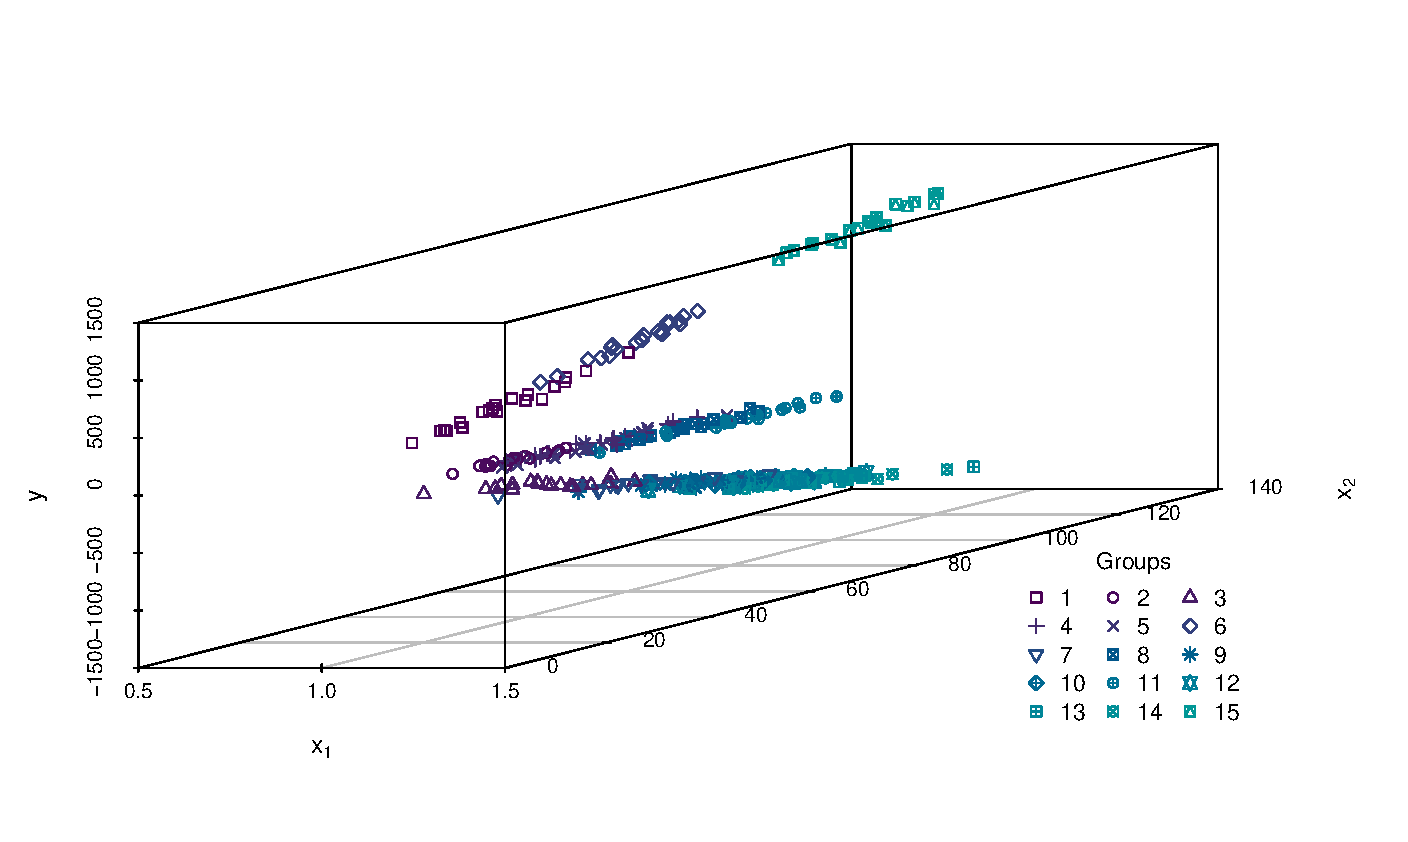
\includegraphics[scale=0.5]{Kap3/chlrm_scatter.pdf}
    \caption{Scatterplot of simulated CHLRM data: response $y$ vs.\ covariates $x_1$ and $x_2$, with group colors.}
    \label{fig:chlrm_scatter}
\end{figure}

Figure~\ref{fig:chlrm_scatter} illustrates the separation of the simulated groups in covariate–response space. This geometric heterogeneity facilitates identifiability of cluster–specific coefficients $(\bm{\beta}_k,\sigma_k^2)$ and underpins the subsequent parameter recovery.


\begin{figure}[H]
    \centering
    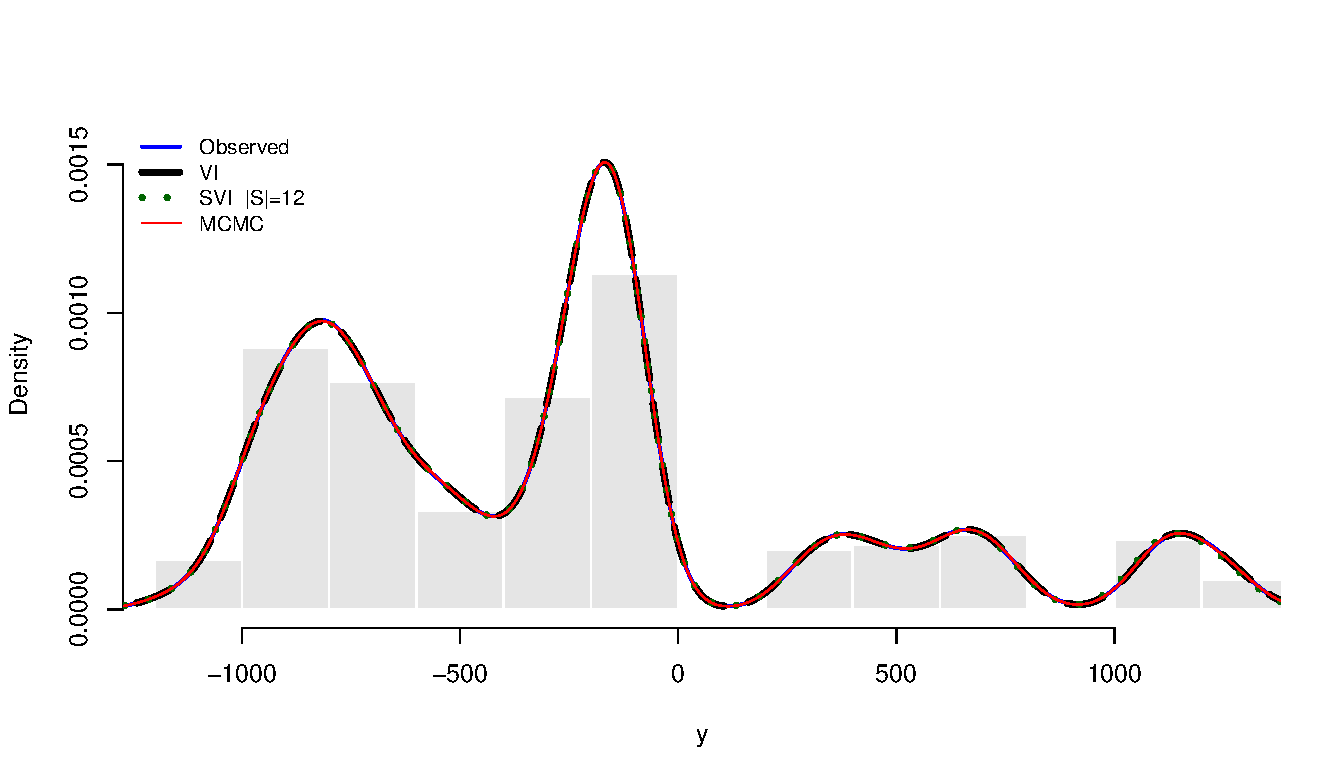
\includegraphics[scale=0.55]{Kap3/chlrm_y_density_sim.pdf}
    \caption{Observed $y$ and posterior predictive densities (MCMC, VI, SVI), simulated data.}
    \label{fig:chlrm_y_density_sim}
\end{figure}

Figure~\ref{fig:chlrm_y_density_sim} shows the multimodal distribution induced by the three regression components. The posterior predictive densities of MCMC, VI, and SVI recover the bulk of the distribution, although VI and SVI display slightly lighter tails, a feature consistent with the mean–field approximation. This predictive fit is consistent with the evidence in Table~\ref{tab:fit_chlrm}, where the MSE and $\mathsf{R}^2$ are broadly comparable across methods. The only notable deviation is the MSE under SVI, which is elevated owing to inflated variability for cluster 1 induced by the mean-field factorization (i.e., the approximation’s neglect of posterior dependencies)..

\begin{figure}[H]
    \centering
    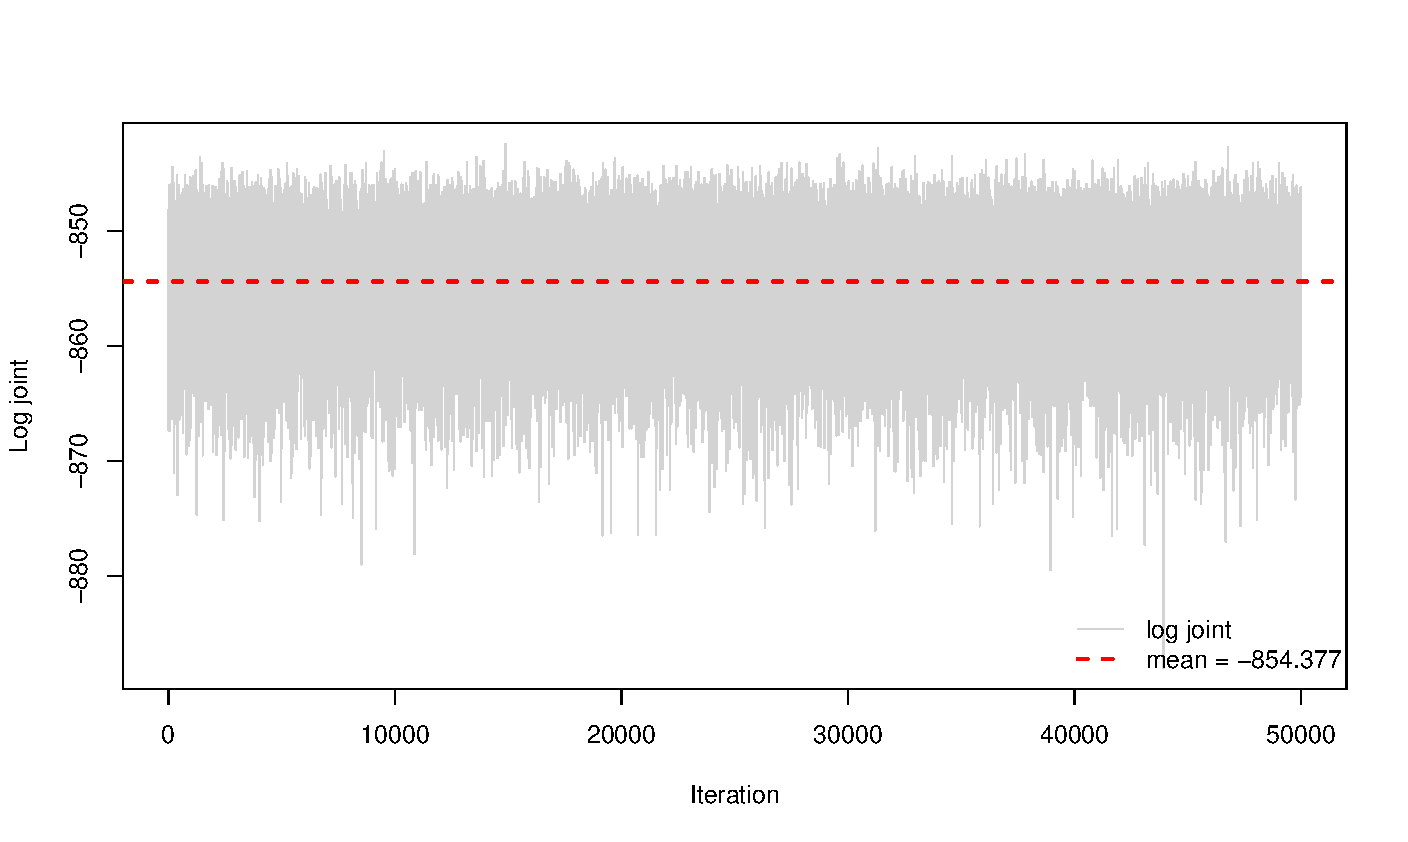
\includegraphics[scale=0.45]{Kap3/chlrm_logjoint_chain.pdf}
    \caption{Trace of the log-joint distribution under MCMC estimation, simulated data.}
    \label{fig:chlrm_logjoint_chain}
\end{figure}

\begin{algorithm}[H]
\scriptsize 
\caption{SVI for CHLRM}
\label{SVI_CHLRM_alg}
\begin{algorithmic}
\State \textbf{Input} Init values $
\{\bm{\mu}_{\bm{\beta}_k}^{(0)},\bm{\Sigma}_{\bm{\beta}_k}^{(0)}\}_{k=1}^K,\;
\bm{\mu}_{\bm{\beta}}^{(0)},\;\bm{\Sigma}_{\bm{\beta}}^{(0)},\;
\nu_{\bm{\Sigma}},\bm{S}_{\bm{\Sigma}}^{(0)},\;
a_{\xi^2}, b_{\xi^2}^{(0)},\;
\{a_{\sigma_k^2}^{(0)}, b_{\sigma_k^2}^{(0)}\}_{k=1}^K,\;
\{\rho_{jk}^{(0)}\}_{j=1}^m,\;
\bm{\alpha}^{(0)}_{\bm{\omega}}$, hyperparameters $\bm{\mu}_0,\bm{\Lambda}_0,n_0,\bm{S}_0,a_0,b_0,\nu_0,\bm{\alpha}_0$, learning rate parameters $\tau,\chi$, minibatch size $|\mathcal{S}|$, number of iterations $T$

\For{$t = 1,\dots,T$}
\State \textbf{\textit{Local updates}}
  \State Select a mini-batch of groups $\mathcal{S} \subset \{1,\dots,m\}$.
  \For{$j \in \mathcal{S}$}
    \State Update $q(\gamma_j)$ setting $\rho_{jk}^{(t)}$ (eq. \ref{CHLRM_CAVI_rhojk_gamma}).
  \EndFor
  \State  Calculate step size  $\rho_t = (t+\tau)^{-\chi}$
  \State \textbf{\textit{Noisy Gradients}}
  \State Calculate Intermediate global parameters
  $$
    \hat{\bm{\Sigma}_{\bm{\beta}_k}}^{-1} =  \mathsf{E}_{\bm{\Sigma}}\left[\bm{\Sigma}^{-1}\right]+\mathsf{E}_{\sigma^2_k}\left[{\sigma_k}^{-2}\right] \tfrac{m}{|\mathcal{S}|}\sum_{j \in \mathcal{S}} \mathsf{E}_{\gamma_j}\left[[\gamma_j=k]\right]\bm{X}_{j}^\top \bm{X}_{j}
  ,\quad
  \hat{\bm{\mu}_{\bm{\beta}_k}} =\hat{\bm{\Sigma}_{\bm{\beta}_k}}\left( \bm{\Lambda}_0^{-1} \bm{\mu}_0 +\tfrac{m}{|\mathcal{S}|}\sum_{j \in \mathcal{S}} \sum_{k=1}^K  \mathsf{E}_{\bm{\Sigma}}\left[\bm{\Sigma}^{-1}\right] \mathsf{E}_{\bm{\beta}_k}\!\left[\bm{\beta}_k \right]\right)
  $$
    $$
    \hat{a_{\sigma^2_k}} =  \frac{\nu_0}{2} + \frac{1}{2}\tfrac{m}{|\mathcal{S}|}\sum_{j \in \mathcal{S}}\mathsf{E}_{\gamma_j}\left[[\gamma_j=k]\right]n_j
  ,\quad
  \hat{b_{\sigma_k^2}} =\frac{ \nu_0 }{2}\mathsf{E}_{\xi^2}\left[\xi^2\right] +  \frac{1}{2}\tfrac{m}{|\mathcal{S}|}\sum_{j \in \mathcal{S}}\mathsf{E}_{\gamma_j}\left[[\gamma_j=k]\right]\mathsf{E}_{\bm{\beta}_k}\left[\left(\bm{y}_{j} - \bm{X}_{j} \bm{\beta}_k\right)^\top\left(\bm{y}_{j} - \bm{X}_{j} \bm{\beta}_k\right)\right]
  $$
    $$
    \hat{\bm{\Sigma}_{\bm{\beta}}}^{-1} = \bm{\Lambda}_0^{-1} + \sum_{k=1}^K 
  \mathsf{E}_{\bm{\Sigma}}\left[\bm{\Sigma}^{-1}\right]
  ,\quad
  \hat{\bm{\mu}_{\bm{\beta}}} =\hat{\bm{\Sigma}_{\bm{\beta}}}\left( \bm{\Lambda}_0^{-1} \bm{\mu}_0 +\sum_{k=1}^K  \mathsf{E}_{\bm{\Sigma}}\left[\bm{\Sigma}^{-1}\right] \mathsf{E}_{\bm{\beta}_k}\!\left[\bm{\beta}_k \right]\right)
  $$
  $$
  \hat{\bm{S}_{\bm{\Sigma}}} = \bm{S}_0+ \sum_{k=1}^K  \mathsf{E}_{\bm{\beta}_k,\bm{\beta}}\!\left[(\bm{\beta}_k-\bm{\beta})(\bm{\beta}_k-\bm{\beta})^\top\right],
  \quad 
  \hat{b_{\xi^2}} =b_0 + \tfrac{\nu_0}{2} \sum_{k=1}^K 
  \mathsf{E}_{\sigma_k^2}\left[\sigma_k^{-2}\right]
  $$
  $$
  \hat{\bm{\alpha}_{\bm{\omega}}} = \bm{\alpha}_0+\tfrac{m}{|\mathcal{S}|}\sum_{j \in \mathcal{S}}\left(\mathsf{E}_{\gamma_j}\left[[\gamma_j=1]\right],\cdots,\mathsf{E}_{\gamma_j}\left[[\gamma_j=K]\right]\right)^\top
  $$

  \State \textbf{\textit{Global updates}}

  \For{$k=1,\dots,K$}
  \State Update $q(\bm{\beta}_k)$ setting 
  $$
  \left(\bm{\Sigma}_{\bm{\beta}_k}^{-1}\right)^{(t)} \leftarrow (1-\rho_t)\left(\bm{\Sigma}_{\bm{\beta}_k}^{-1}\right)^{(t-1)} + \rho_t\left(\hat{\bm{\Sigma}_{\bm{\beta}_k}}^{-1}\right)^{(t)}
  $$
  \State
  $$
  \bm{\mu}_{\bm{\beta}_k}^{(t)} \leftarrow (1-\rho_t)\,\bm{\mu}_{\bm{\beta}_k}^{(t-1)} + \rho_t   \hat{\bm{\mu}_{\bm{\beta}_k}}^{(t)}
  $$
    \State Update $q(\sigma^2_k)$ setting 
  $$
  {a_{\sigma_k^2}}^{(t)} \leftarrow (1-\rho_t){a_{\sigma_k^2}}^{(t-1)} + \rho_t\hat{{a_{\sigma_k^2}}}^{(t)}
  $$
  \State
  $$
  {b_{\sigma_k^2}}^{(t)} \leftarrow (1-\rho_t){b_{\sigma_k^2}}^{(t-1)} + \rho_t   \hat{{b_{\sigma_k^2}}}^{(t)}
  $$
    \EndFor
    \State Update $q(\bm{\omega})$ setting 
  $$
  \bm{\alpha}_{\bm{\omega}}^{(t)} \leftarrow (1-\rho_t)\, \bm{\alpha}_{\bm{\omega}}^{(t-1)} + \rho_t \hat{\bm{\alpha}_{\bm{\omega}}}^{(t)}
  $$
  
  \State Update $q (\bm{\beta})$ setting
  $$
  \left(\bm{\Sigma}_{\bm{\beta}}^{-1}\right)^{(t)} \leftarrow (1-\rho_t)\left(\bm{\Sigma}_{\bm{\beta}}^{-1}\right)^{(t-1)} + \rho_t  \left(\hat{\bm{\Sigma}_{\bm{\beta}}}^{-1}\right)^{(t)}
  $$
  \State
  $$
  \bm{\mu}_{\bm{\beta}}^{(t)} \leftarrow (1-\rho_t)\,\bm{\mu}_{\bm{\beta}}^{(t-1)} + \rho_t   \hat{\bm{\mu}_{\bm{\beta}}}^{(t)}
  $$
  \State Update $q (\bm{\Sigma})$ setting
  $$
  \bm{S}_{\bm{\Sigma}}^{(t)} \leftarrow (1-\rho_t)\,\bm{S}_{\bm{\Sigma}}^{(t-1)} + \rho_t \hat{\bm{S}_{\bm{\Sigma}}}^{(t)}
  $$
  \State Update $q (\xi^2)$ setting
  $$
  b_{\xi^2}^{(t)} \leftarrow (1-\rho_t)\,b_{\xi^2}^{(t-1)} + \rho_t \hat{b_{\xi^2}}^{(t)}
  $$
\EndFor
\State \textbf{Output}  Optimal parameters $
\{\bm{\mu}_{\bm{\beta}_k},\bm{\Sigma}_{\bm{\beta}_k}\}_{k=1}^K,
\bm{\mu}_{\bm{\beta}},\bm{\Sigma}_{\bm{\beta}},
\bm{S}_{\bm{\Sigma}},
\{a_{\sigma_k^2}, b_{\sigma_k^2}\}_{k=1}^K,
a_{\xi^2}, b_{\xi^2},
\{\rho_{jk}\}_{j=1}^m,\bm{\alpha}_{\bm{\omega}}$
\end{algorithmic}
\end{algorithm}

\begin{figure}[H]
    \centering
    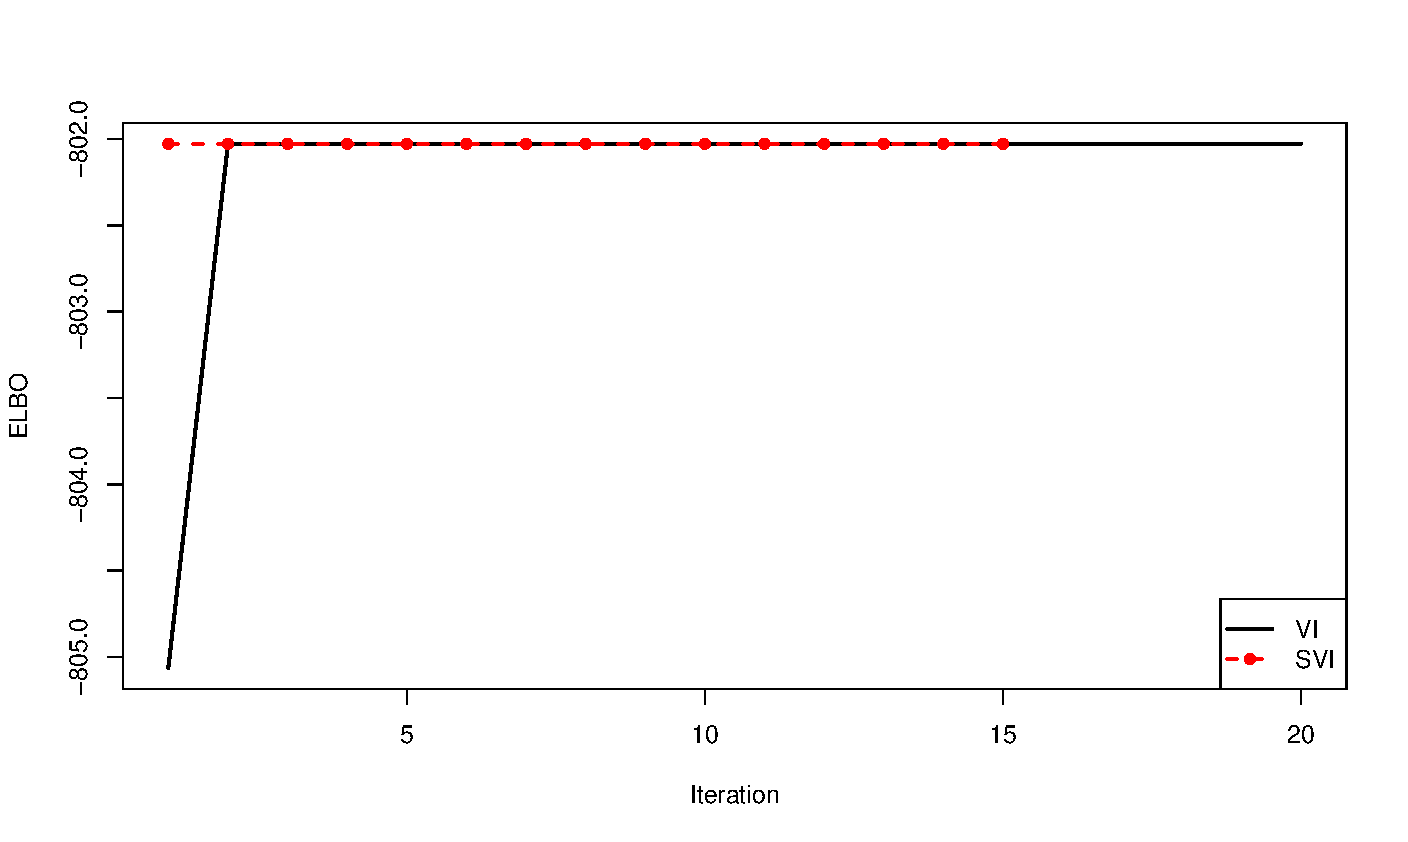
\includegraphics[scale=0.45]{Kap3/chlrm_elbo_vi_svi.pdf}
    \caption{ELBO across iterations: VI  vs.\ SVI $|S|=12$, $\epsilon=1\times10^{-7}\%,\ \chi = 0.7,\ \tau = 71.2$, simulated data.}
    \label{fig:chlrm_elbo_vi_svi}
\end{figure}

Figures~\ref{fig:chlrm_logjoint_chain}–\ref{fig:chlrm_elbo_vi_svi} assess convergence. The MCMC chain stabilizes after burn–in with a stationary mean around $-854$, evidencing satisfactory mixing. VI exhibits a smooth ascent of the ELBO, while SVI converges more erratically but to a similar bound. Together with the runtimes reported in Table~\ref{tab:fit_chlrm}, these plots highlight the trade–off: MCMC provides faithful posterior sampling but at high cost (466s), while VI and SVI achieve similar predictive performance in fractions of a second.

\begin{figure}[H]
    \centering
    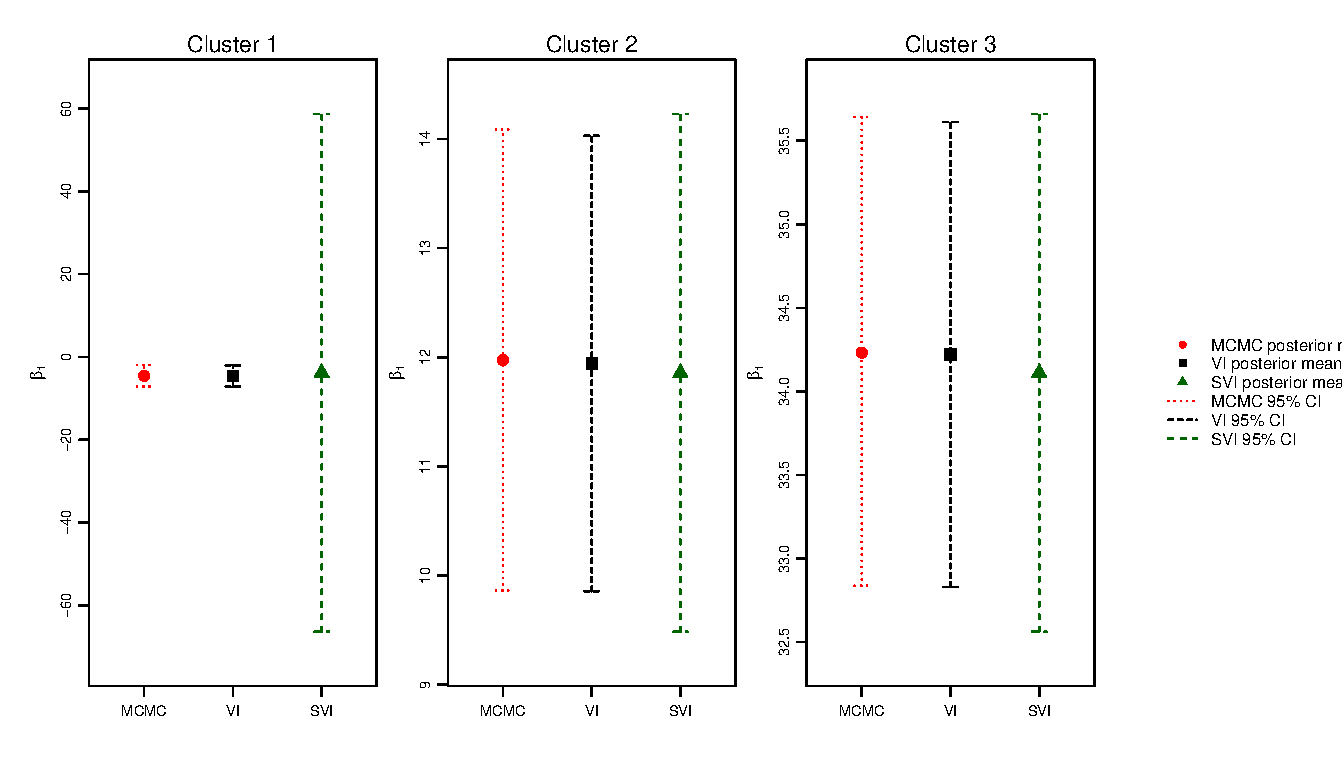
\includegraphics[scale=0.7]{Kap3/chlrm_beta1.pdf}
    \caption{Posterior summaries of $\beta_{1}$ across clusters, simulated data.}
    \label{fig:chlrm_beta1}
\end{figure}

\begin{figure}[H]
    \centering
    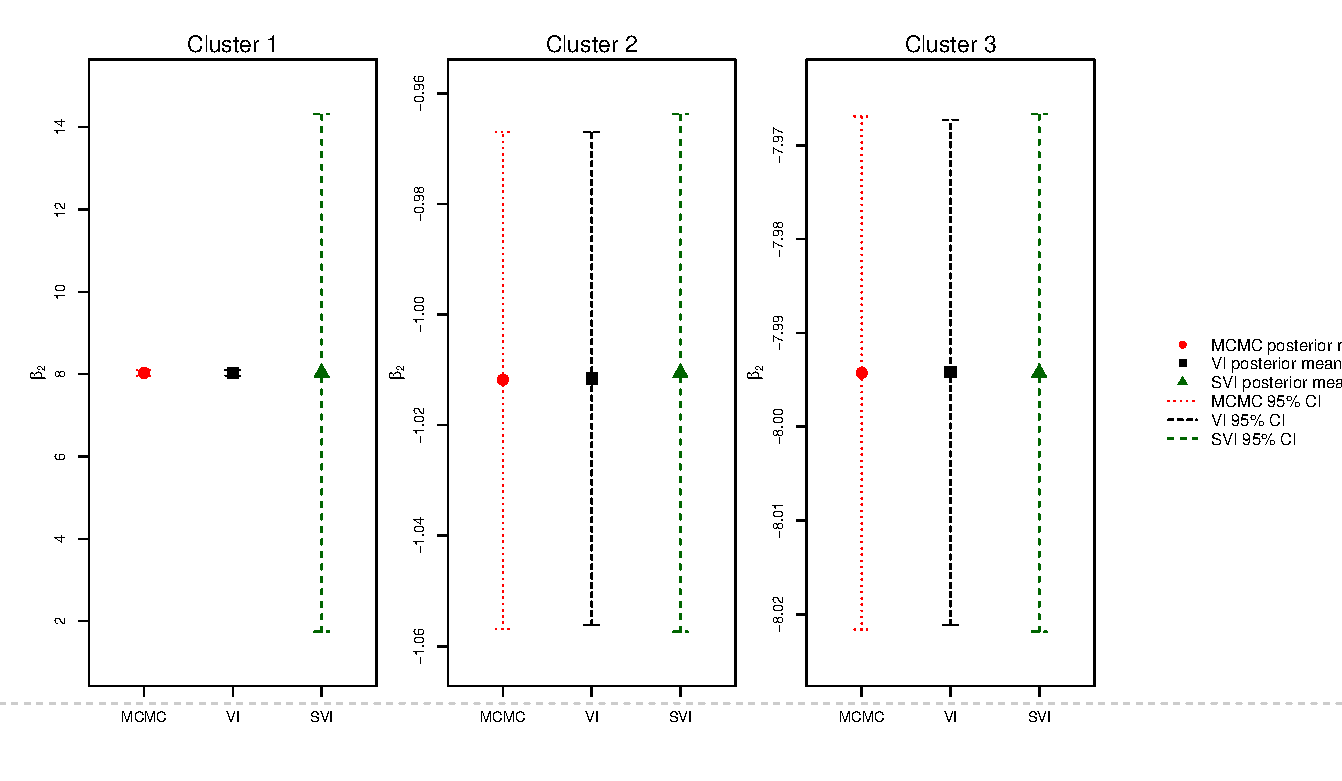
\includegraphics[scale=0.7]{Kap3/chlrm_beta2.pdf}
    \caption{Posterior summaries of $\beta_{2}$ across clusters, simulated data.}
    \label{fig:chlrm_beta2}
\end{figure}

Figures~\ref{fig:chlrm_beta1}–\ref{fig:chlrm_sigma2} confirm accurate recovery of regression slopes and error variances. Posterior means align closely with the true values, while credible intervals differ across methods: MCMC provides wider and better–calibrated intervals, whereas VI and SVI underestimate uncertainty, a known limitation of factorized approximations. This discrepancy is particularly evident for Cluster~1, where higher variability amplifies uncertainty. Nevertheless, the accuracy metrics in Table~\ref{tab:fit_chlrm} confirm the adequacy of all three methods.



\begin{table}[!h]
\centering
\caption{Goodness of fit and runtime (CHLRM, 1000 posterior samples), simulated data.}
\label{tab:fit_chlrm}
\begin{tabular}{@{} l l r r r r r @{}}
\toprule
\textbf{Method} & \textbf{Settings} & \textbf{WAIC} & \textbf{DIC} & \textbf{MSE} & \textbf{$\bm{\mathsf{R}}^2$} & \textbf{Time (s)}\\
\midrule
MCMC &
\begin{tabular}{@{}l@{}}
samples: 50000\\
burn-in: 10000\\
thin: 10
\end{tabular}
& 1453.311 & 1453.671 & 8.023 & 1 & 466.055\\
\midrule
VI &
\begin{tabular}{@{}l@{}}
iterations: 20\\
$\epsilon=1\times10^{-7}\%$
\end{tabular}
& 1453.323 & 1453.570 & 8.022 & 1 & 0.198\\
\midrule
SVI &
\begin{tabular}{@{}l@{}}
iterations: 15\\
$\epsilon=1\times10^{-7}\%$\\
$|S| = 12,\ \chi = 0.7,\ \tau = 25.8$
\end{tabular}
& 1983.810 & 2028.781 & 11.344 & 1 & 0.02\\
\bottomrule
\end{tabular}
\end{table}


\begin{figure}[H]
    \centering
    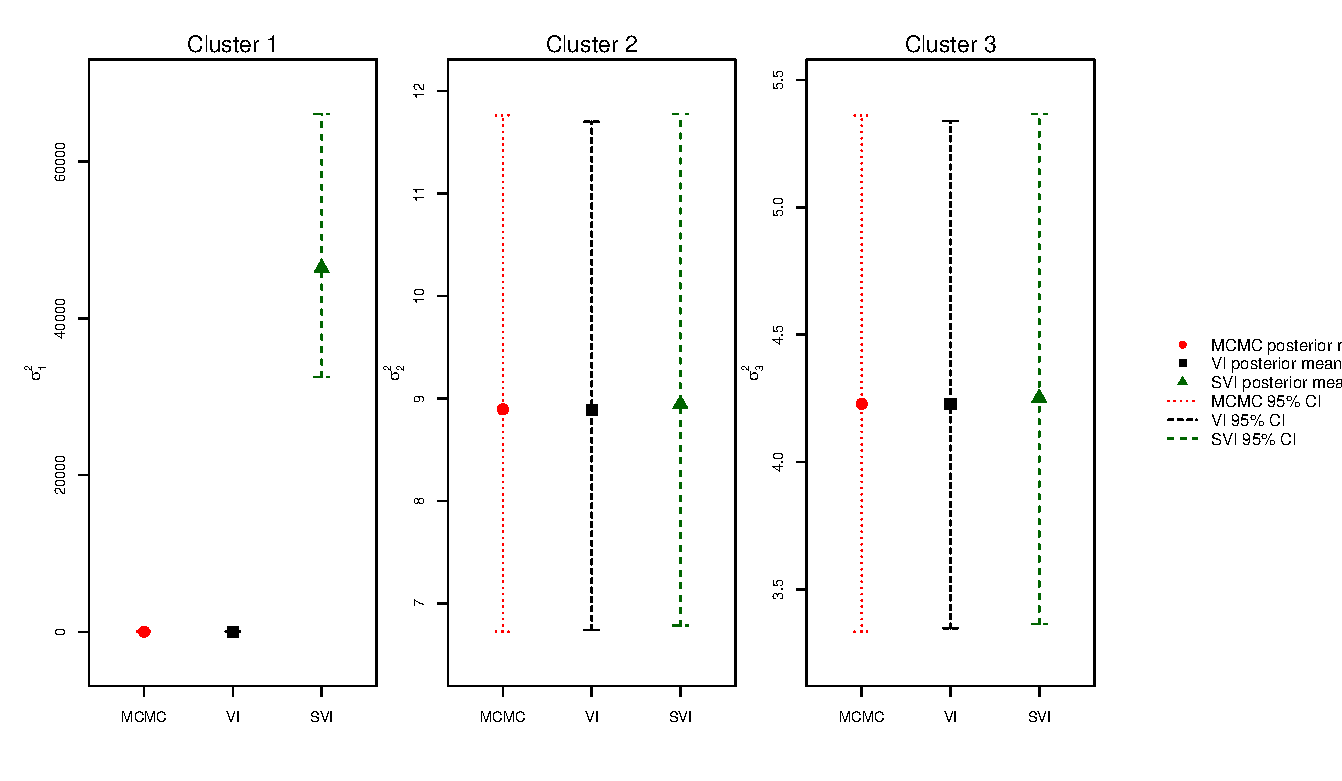
\includegraphics[scale=0.7]{Kap3/chlrm_sigma2.pdf}
    \caption{Posterior summaries of $\sigma^2_k$ across clusters , simulated data.}
    \label{fig:chlrm_sigma2}
\end{figure}



\noindent Taken together, Tables~\ref{tab:fit_chlrm} and~\ref{tab:ppp} indicate that the three inference strategies achieve nearly identical predictive accuracy. WAIC and DIC values remain virtually the same across MCMC, VI, and SVI, while MSE and $R^2$ confirm that the fitted models explain almost all of the variability in the simulated data. The posterior predictive $p$-values further reinforce this agreement: all methods yield values close to 0.5, reflecting replicated data that is statistically consistent with the observed outcomes. The combination of stable information criteria, negligible predictive error, and balanced $p_{pp}$ values demonstrates that even though VI and SVI operate under stronger approximating assumptions and achieve dramatic computational savings their predictive adequacy is not compromised relative to the gold standard provided by MCMC.

\begin{table}[!h]
\centering
\caption{\label{tab:ppp}Posterior predictive $p$-values for CHLRM (1000 replications), simulated data.}
\begin{tabular}{@{} lrrrrrr @{}}
\toprule
\textbf{Method} & \textbf{min} & \textbf{max} & \textbf{IQR} & \textbf{mean} & \textbf{median} & \textbf{sd} \\
\midrule
MCMC &  0.75 & 0.79 & 0.37 & 0.48 & 0.65 & 0.48\\
VI   & 0.73 & 0.78 & 0.35 & 0.48 & 0.65 & 0.50\\
SVI  & 0.73 & 0.79 & 0.23 & 0.50 & 0.61 & 0.53\\
\bottomrule
\end{tabular}
\end{table}


\begin{figure}[H]
    \centering
    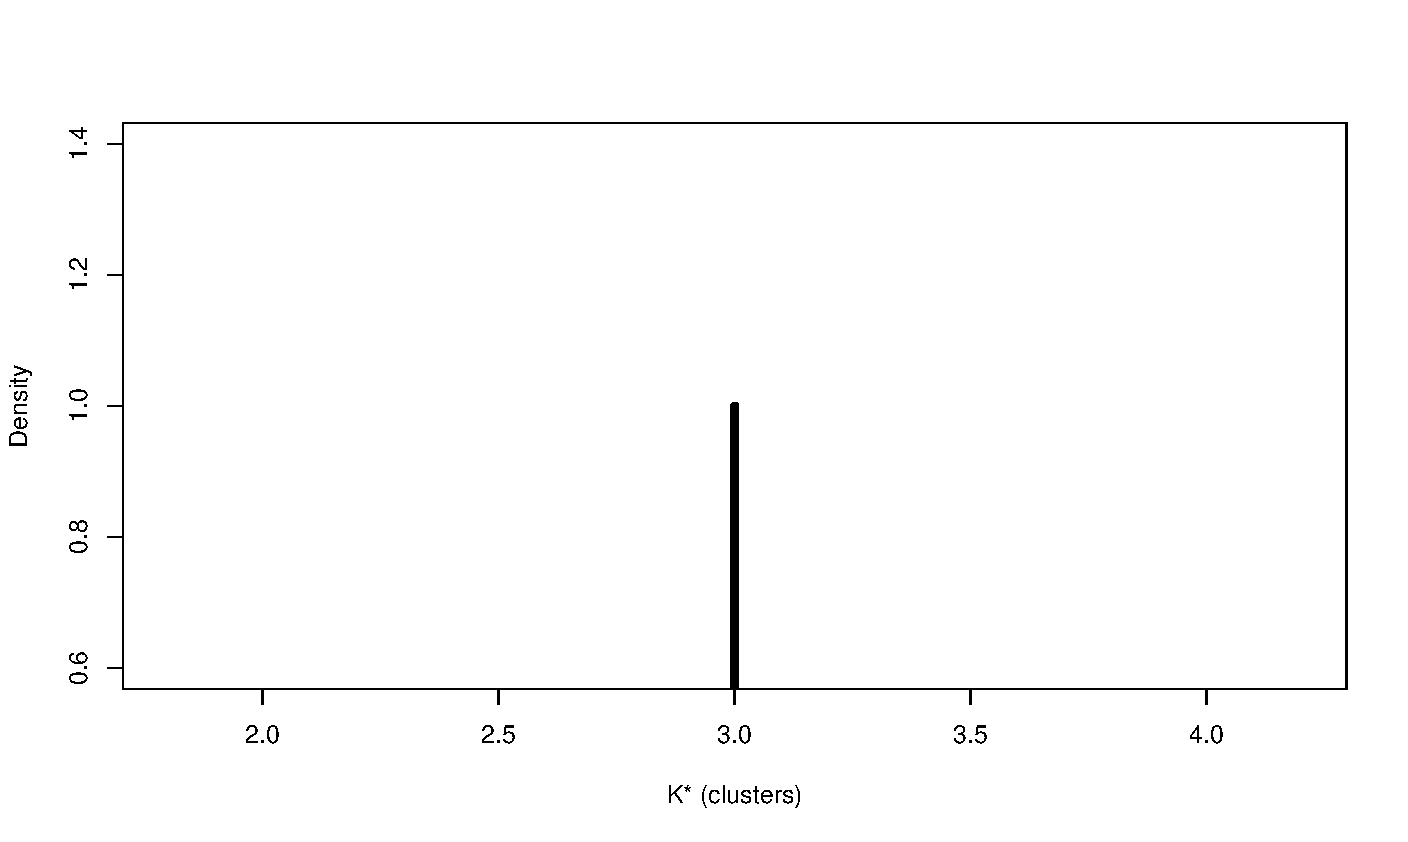
\includegraphics[scale=0.55]{Kap3/chlrm_mcmc_k.pdf}
    \caption{Posterior density of the number of non–empty clusters under MCMC with $K=14$, 50000 samples, 10000 burn-in iterations and thinned each 10 iterations, simulated data.}
    \label{fig:chlrm_mcmc_k}
\end{figure}

To get the partition size, two complementary analyses were performed. First, an MCMC run with $K=14$ estimated the posterior distribution of the number of non empty clusters (Figure~\ref{fig:chlrm_mcmc_k}), which concentrated its mass on $K=3$. Second, VI was run varying $K=1,\dots,14$ under the settings of Table~\ref{tab:fit_chlrm}; Figure~\ref{fig:chlrm_vi_k} shows that the ELBO is maximized at $K=3$, degrading for larger values. Both diagnostics consistently support the true number of clusters.

\begin{figure}[H]
    \centering
    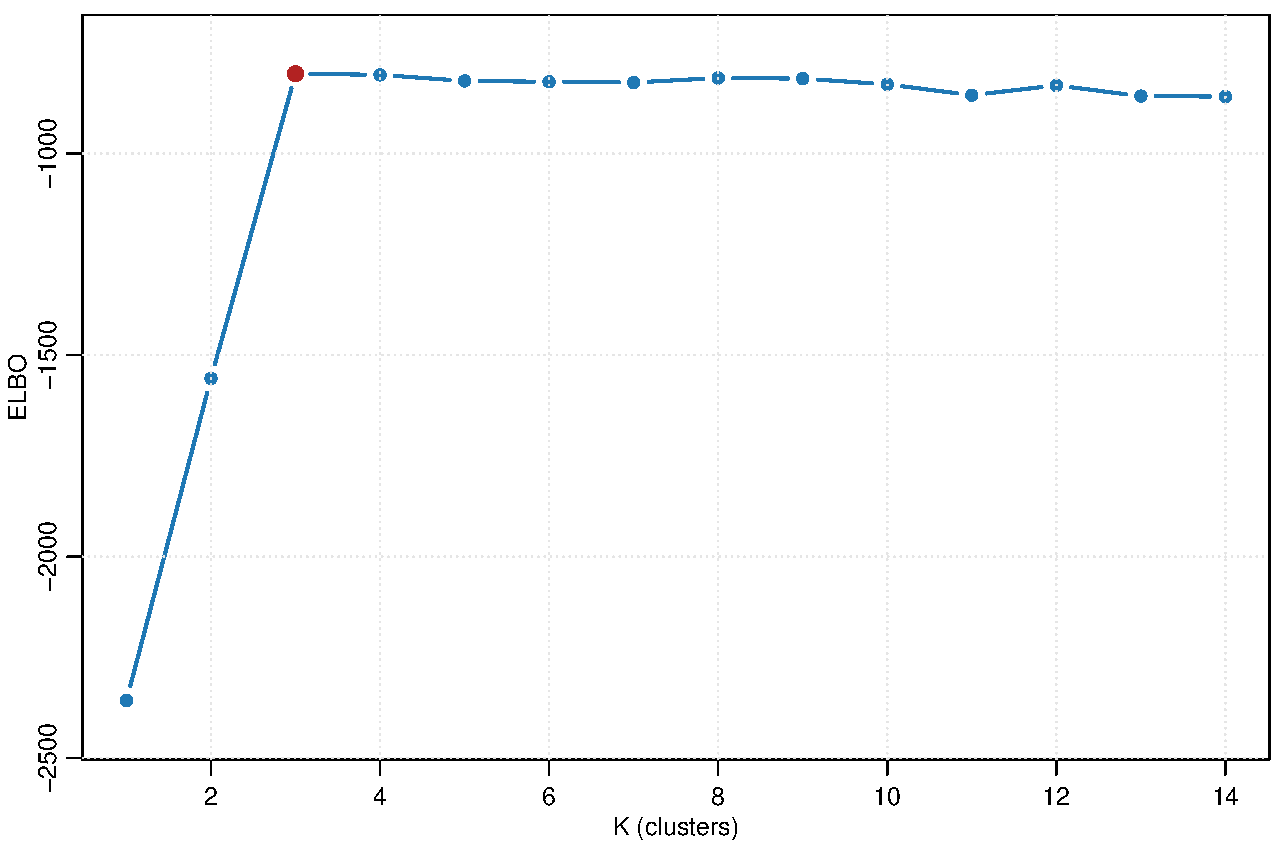
\includegraphics[scale=0.55]{Kap3/chlrm_vi_k.pdf}
    \caption{ELBO values vs.\ $K$ , simulated data.}
    \label{fig:chlrm_vi_k}
\end{figure}

The adjacency matrices in Figure~\ref{fig:chlrm_adjacency_compare} illustrate the evolution from a diffuse initialization to a clear block–diagonal structure, evidencing recovery of the true $K=3$ partition. This structural evidence complements the density fit in Figure~\ref{fig:chlrm_y_density_sim}, the parameter recovery in Figures~\ref{fig:chlrm_beta1}–\ref{fig:chlrm_sigma2}, and the metrics in Table~\ref{tab:fit_chlrm}, confirming that all methods converge to the same clustering solution, with MCMC providing the most reliable uncertainty quantification and VI/SVI offering substantial computational efficiency.

\begin{figure}[H]
    \centering
    \begin{minipage}{0.48\textwidth}
        \centering
        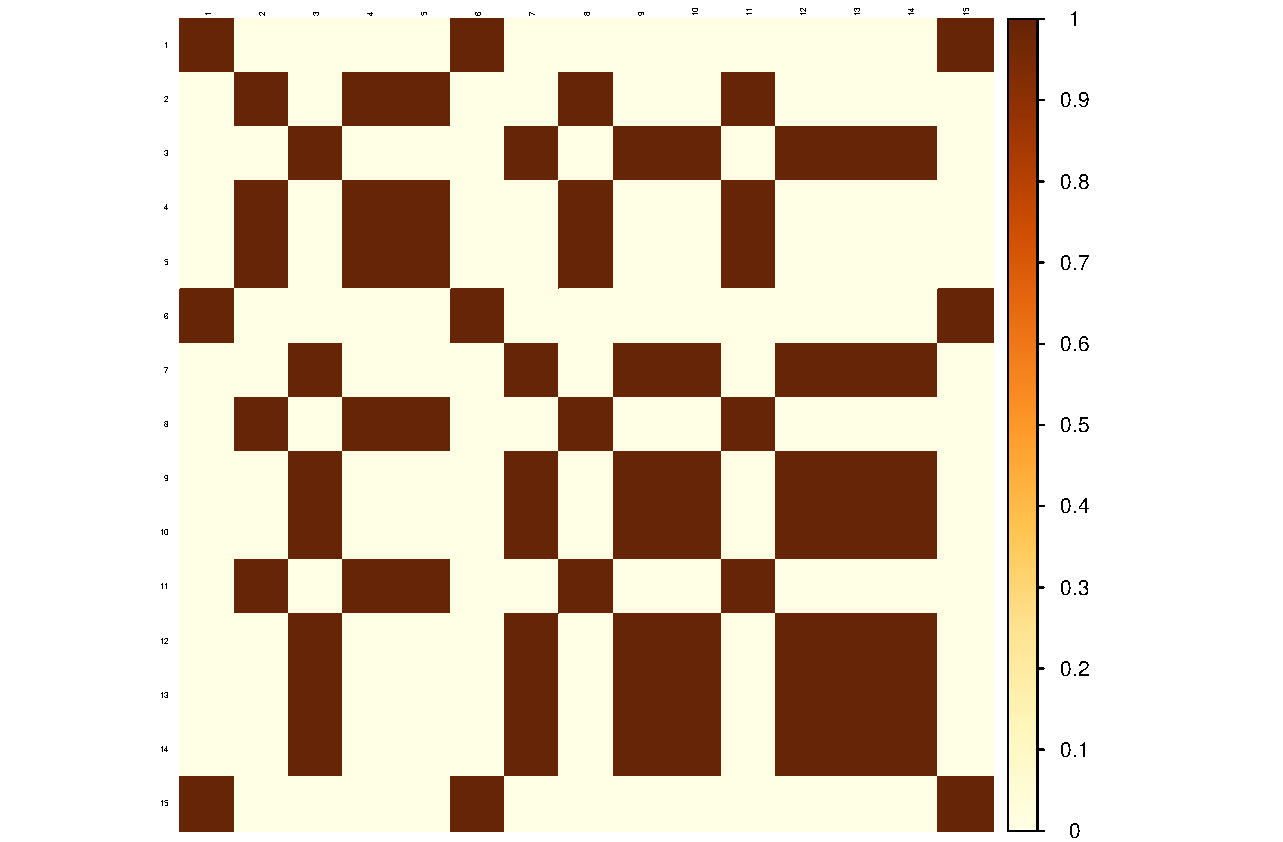
\includegraphics[width=\textwidth]{Kap3/chlrm_adjacency_init.pdf}
        \caption*{(a) Initial adjacency}
    \end{minipage}\hfill
    \begin{minipage}{0.48\textwidth}
        \centering
        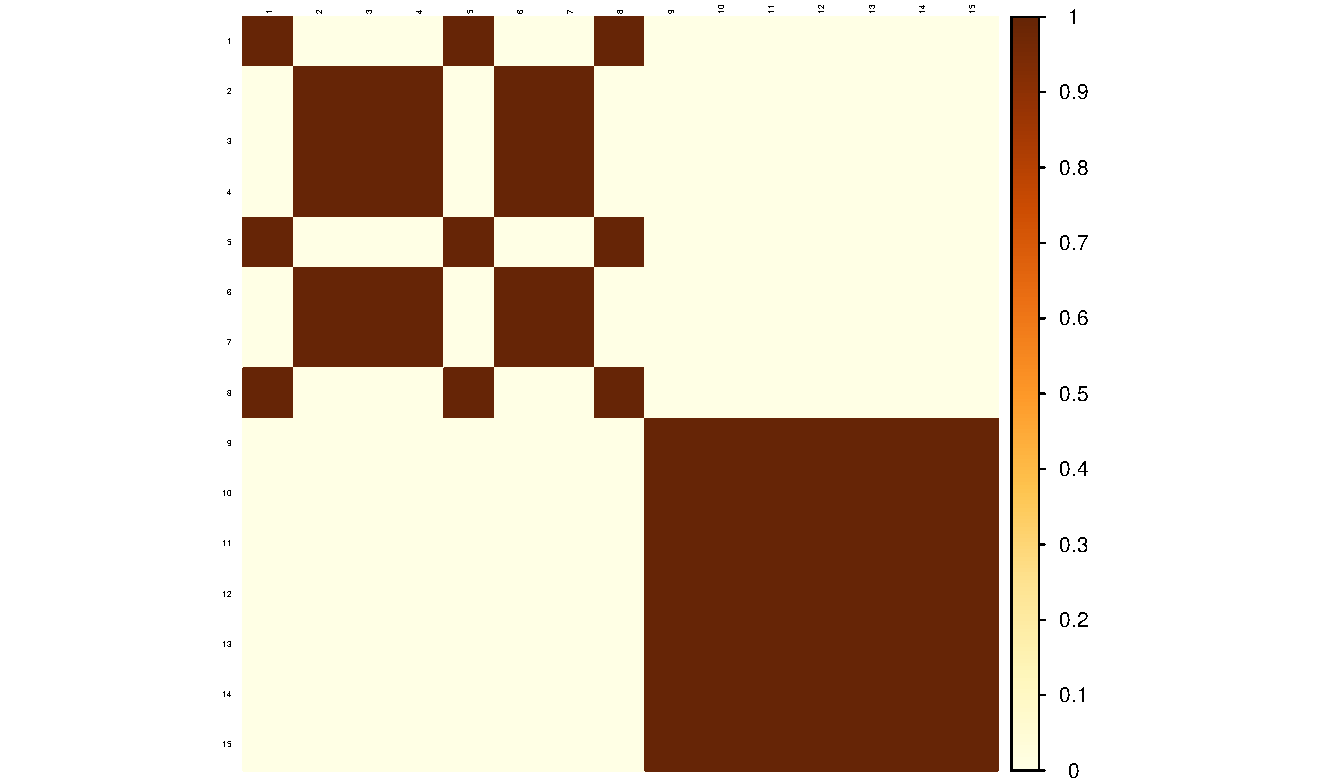
\includegraphics[width=\textwidth]{Kap3/chlrm_adjacency_final.pdf}
        \caption*{(b) Final adjacency}
    \end{minipage}
    \caption{Adjacency matrices: co–assignment probabilities between groups, simulated data.}
    \label{fig:chlrm_adjacency_compare}
\end{figure}

\subsubsection{Farms Dataset}

Returning to the farms dataset example (see Subsubsection \ref{farms}), we apply MCMC, VI, and SVI to the CHLRM with the aim of adjusting the posterior density to assess the modeling performance of these methodologies when the cluster separation is not evident. The primary goal is to obtain an optimal partition that explains farm clustering around plant sizes adjusted by soil nitrogen concentration.

\begin{figure}[H]
    \centering
    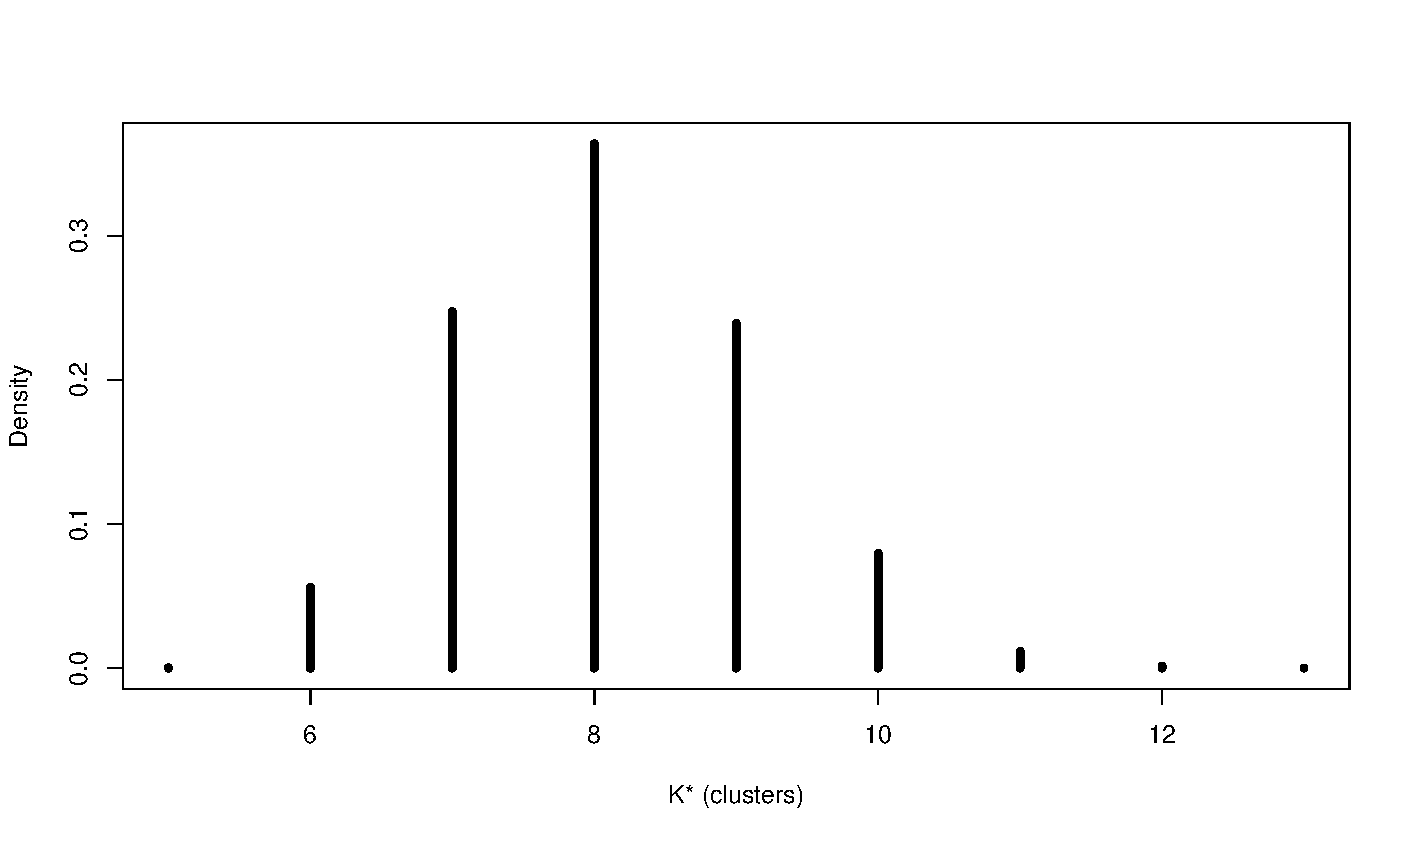
\includegraphics[scale=0.4]{Kap3/chlrm_mcmc_k_farms.pdf}
    \caption{Posterior density of the number of non–empty clusters under MCMC with $K=23$, 50000 samples, 10000 burn–in iterations, and thinning every 10 iterations, farms dataset.}
    \label{fig:chlrm_mcmc_k_farms}
\end{figure}

Figure \ref{fig:chlrm_mcmc_k_farms} shows the posterior density of the number of non–empty clusters, where the most probable values are concentrated around $K \in \{7,8,9\}$. This behavior reflects MCMC’s tendency to favor richer cluster structures, even when empirical separation is not strong. The posterior distribution remains diffuse, suggesting substantial uncertainty in the partitioning. While MCMC is asymptotically exact, its computational burden is considerable, and stabilization of the number of clusters requires long chains and careful thinning. This limitation becomes evident in runtime comparisons later in Table \ref{tab:fit_chlrm_farms}, where MCMC requires several orders of magnitude more time than VI and SVI.

\begin{figure}[H]
    \centering
    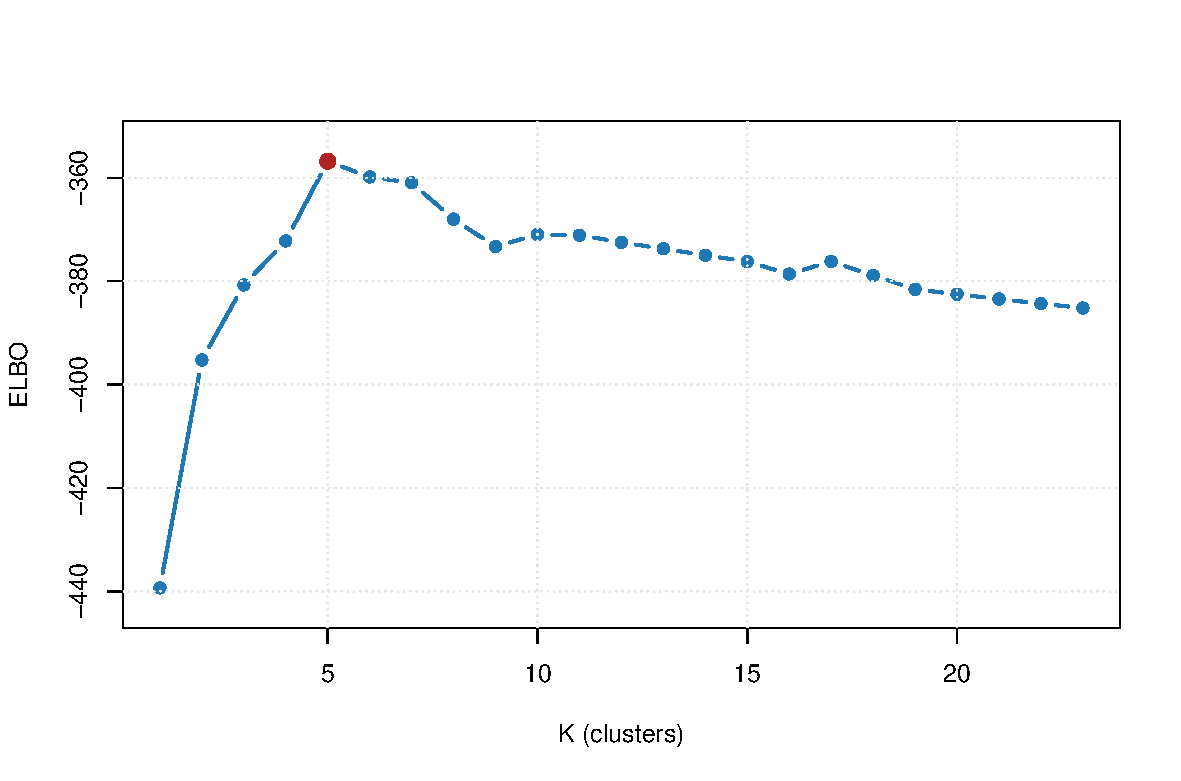
\includegraphics[scale=0.55]{Kap3/chlrm_vi_elbo_k_farms.pdf}
    \caption{ELBO values versus $K$ under SVI ($|S|=18$, $\epsilon=1\times10^{-7}\%$, $\chi = 0.7$, $\tau = 71.2$), farms dataset.}
    \label{fig:chlrm_vi_elbo_k_farms}
\end{figure}

Figure \ref{fig:chlrm_vi_elbo_k_farms} depicts the evolution of the Evidence Lower Bound (ELBO) across different $K$ values. The bound is maximized at $K=5$, favoring a more parsimonious partition compared to the higher cluster counts suggested by MCMC. The smooth trajectory of the ELBO illustrates the deterministic optimization underlying VI and SVI, which converge quickly and with reduced sensitivity to sampling noise. However, it is important to highlight that maximizing ELBO does not guarantee perfect recovery of the true number of clusters. Instead, it balances model complexity and predictive adequacy, providing computational efficiency but often underestimating posterior variance and uncertainty in cluster assignment.

\begin{figure}[H]
    \centering
    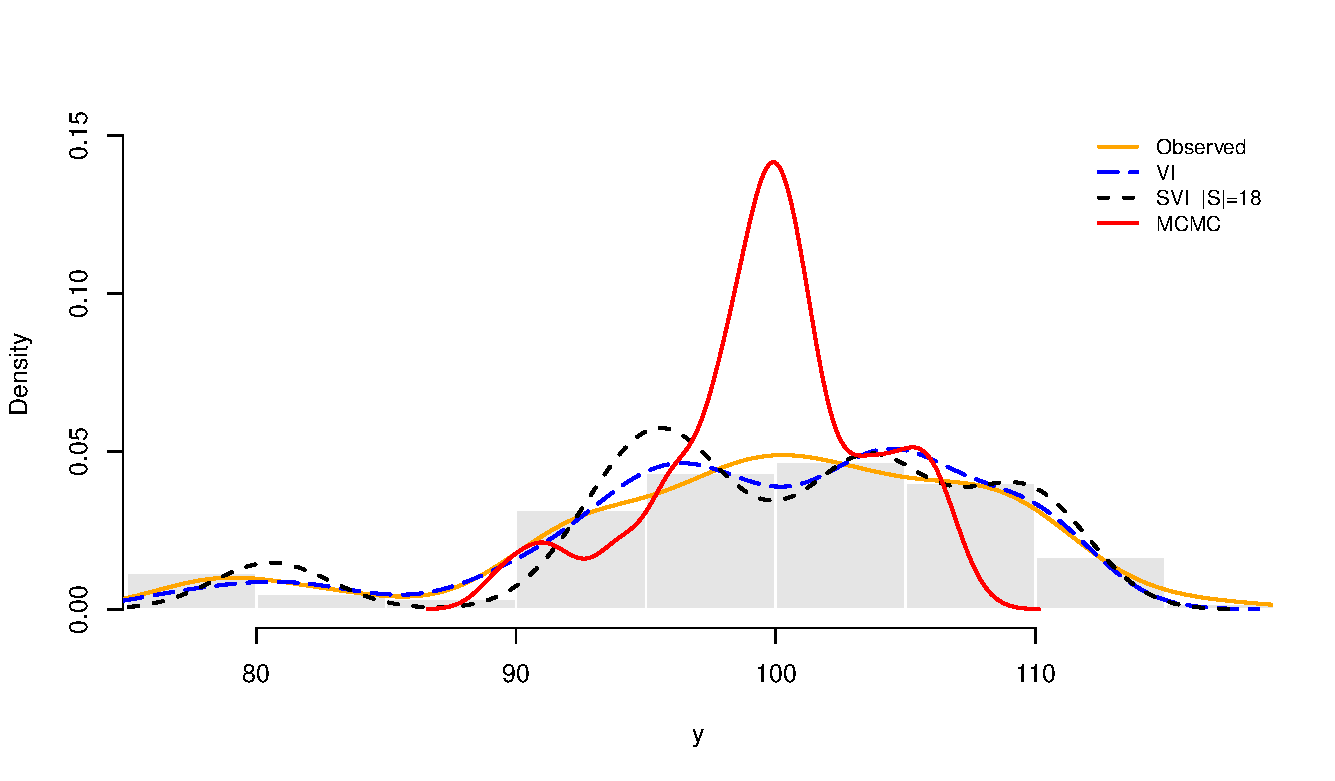
\includegraphics[scale=0.55]{Kap3/chlrm_y_density_farms.pdf}
    \caption{Observed $y$ and posterior predictive densities under MCMC, VI, and SVI with $K=5$ clusters, farms dataset.}
    \label{fig:chlrm_y_density_farms}
\end{figure}

The posterior predictive densities in Figure \ref{fig:chlrm_y_density_farms} show that all three methodologies adequately capture the global shape of the observed $y$. Nonetheless, clear differences emerge. VI and SVI produce sharper and more concentrated predictive distributions, which align more closely with the empirical data. This improved alignment is reflected in their lower MSE and higher $\mathsf{R}^2$ values reported in Table \ref{tab:fit_chlrm_farms}. By contrast, MCMC retains wider tails and higher dispersion, more faithfully representing posterior uncertainty but yielding less precise predictions. This contrast reflects the fundamental methodological trade–off: MCMC excels in posterior fidelity, whereas VI and SVI prioritize computational efficiency and predictive sharpness.

\begin{table}[!h]
\centering
\caption{\label{tab:ppp_farms}Posterior predictive $p$–values for CHLRM (1000 replications), farms dataset.}
\begin{tabular}[t]{llrrrrrr}
\toprule
\textbf{Method} & \textbf{min} & \textbf{max} & \textbf{IQR} & \textbf{mean} & \textbf{median} & \textbf{sd} \\
\midrule
MCMC & 0.34 & 0.33 & 0.23 & 0.50 & 0.46 & 0.56\\
VI & 0.12 & 0.31 & 0.33 & 0.50 & 0.52 & 0.56\\
SVI & 0.13 & 0.19 & 0.30 & 0.56 & 0.58 & 0.64\\
\bottomrule
\end{tabular}
\end{table}

Posterior predictive $p$–values in Table \ref{tab:ppp_farms} reinforce the adequacy of all three methods, as mean and median values are close to 0.5, indicating good calibration of predictive distributions. SVI exhibits slightly higher central values, suggesting an optimistic fit to the observed statistics, consistent with \cite{HOFF}. MCMC produces more balanced values across discrepancy measures, though with greater variability, whereas VI delivers stable but slightly conservative predictive outcomes.

\newpage

\begin{table}[!h]
\centering
\caption{Goodness of fit and runtime (CHLRM, 1000 posterior samples), farms dataset.}
\label{tab:fit_chlrm_farms}
\begin{tabular}{@{} l l r r r r r @{}}
\toprule
\textbf{Method} & \textbf{Settings} & \textbf{WAIC} & \textbf{DIC} & \textbf{MSE} & \textbf{$\bm{\mathsf{R}}^2$} & \textbf{Time (s)}\\
\midrule
MCMC &
\begin{tabular}{@{}l@{}}
samples: 120000\\
burn–in: 30000\\
thin: 20
\end{tabular}
& 570.278 & 583.640 & 30.711 & 0.579 & 3039.362\\
\midrule
VI &
\begin{tabular}{@{}l@{}}
iterations: 11\\
$\epsilon=1\times10^{-7}\%$
\end{tabular}
& 574.070 & 579.002 & 6.330 & 0.913 & 0.020\\
\midrule
SVI &
\begin{tabular}{@{}l@{}}
iterations: 2496\\
$\epsilon=1\times10^{-1}\%$\\
$|S| = 18,\ \chi = 0.7,\ \tau = 71.2$
\end{tabular}
& 615.305 & 624.503 & 5.948 & 0.918 & 3.848\\
\bottomrule
\end{tabular}
\end{table}

Table \ref{tab:fit_chlrm_farms} summarizes the explicit trade–offs. MCMC achieves the lowest WAIC and DIC, underscoring its stronger posterior adherence, but incurs prohibitive runtime (over 3000 seconds). VI and SVI, on the other hand, drastically reduce runtime to fractions of a second or a few seconds, while achieving superior $\mathsf{R}^2$ and lower MSE. Their information criteria values, however, are slightly inflated, reflecting the bias introduced by variational approximations. These results show that the variational algorithms, while highly scalable, may sacrifice posterior fidelity when cluster separation is weak.

\begin{figure}[H]
    \centering
    \begin{minipage}{0.5\textwidth}
        \centering
        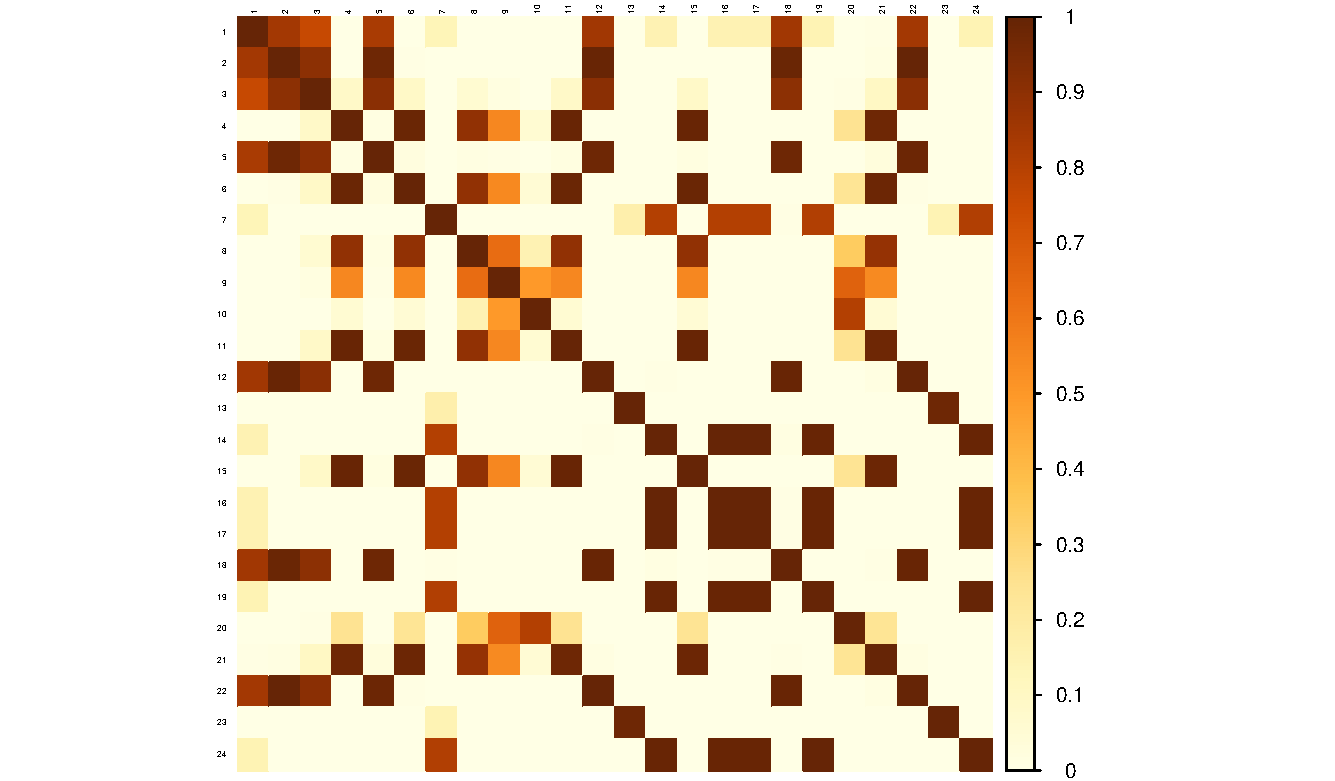
\includegraphics[width=\textwidth]{Kap3/chlrm_mcmc_A_init.pdf}
        \caption*{(a) Initial adjacency}
    \end{minipage}\hfill
    \begin{minipage}{0.5\textwidth}
        \centering
        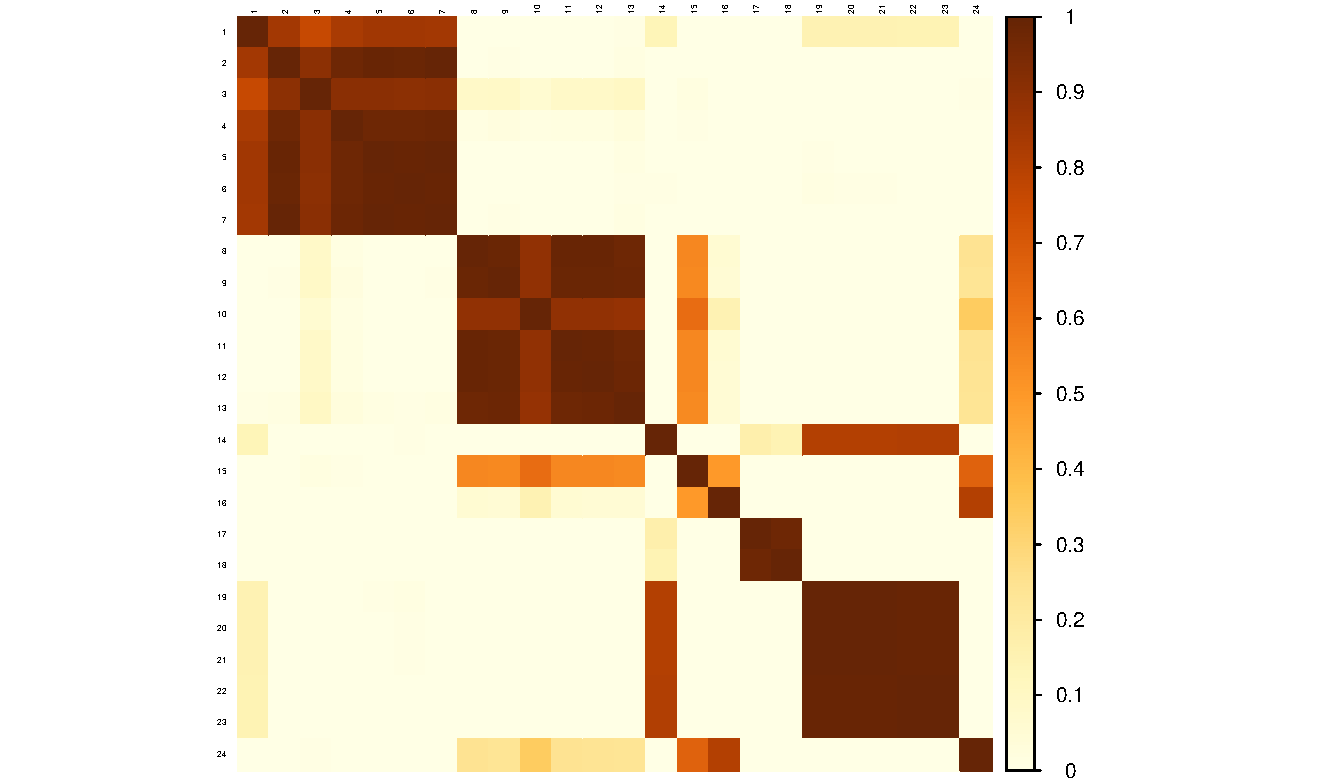
\includegraphics[width=\textwidth]{Kap3/chlrm_mcmc_A_fin.pdf}
        \caption*{(b) Final adjacency}
    \end{minipage}
    \caption{Adjacency matrices: co–assignment probabilities between groups under MCMC, farms dataset.}
    \label{fig:chlrm_mcmc_A_compare}
\end{figure}

\begin{figure}[H]
    \centering
    \begin{minipage}{0.5\textwidth}
        \centering
        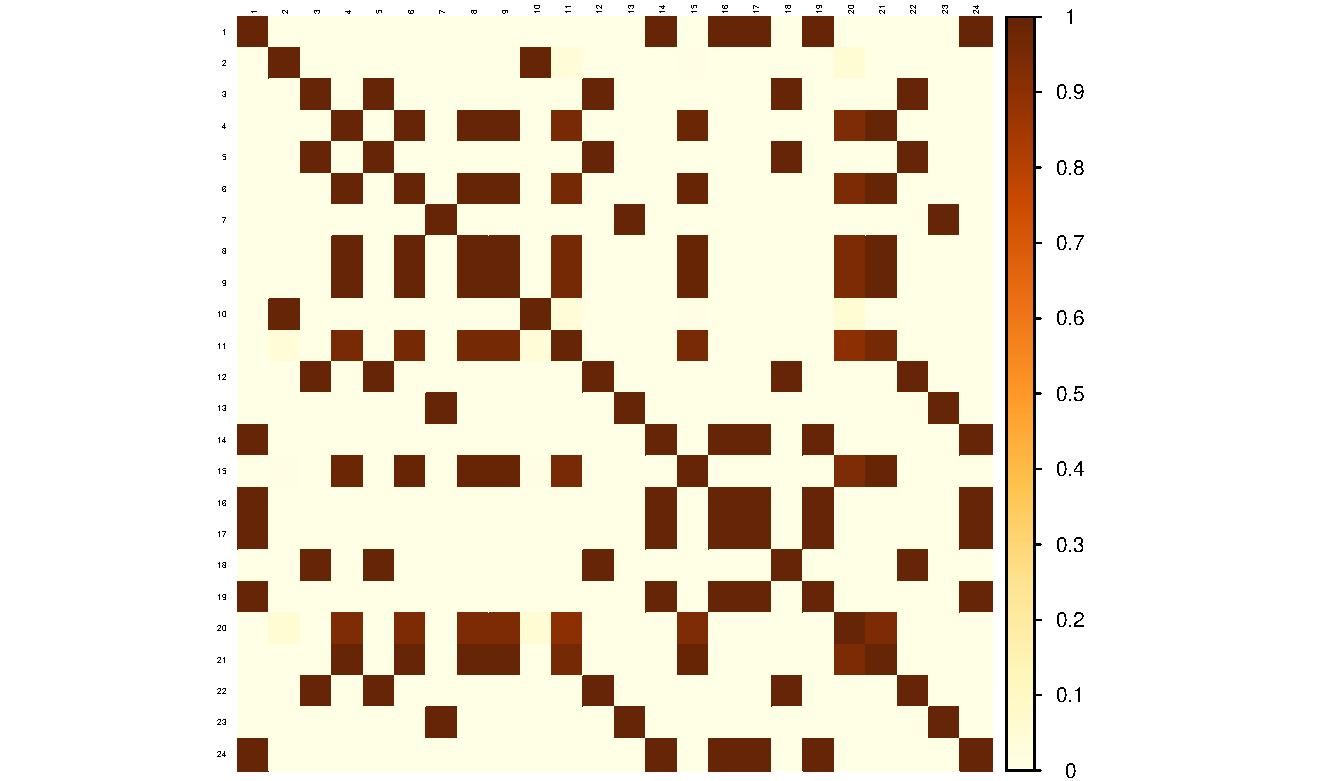
\includegraphics[width=\textwidth]{Kap3/chlrm_vi_A_init.pdf}
        \caption*{(a) Initial adjacency}
    \end{minipage}\hfill
    \begin{minipage}{0.5\textwidth}
        \centering
        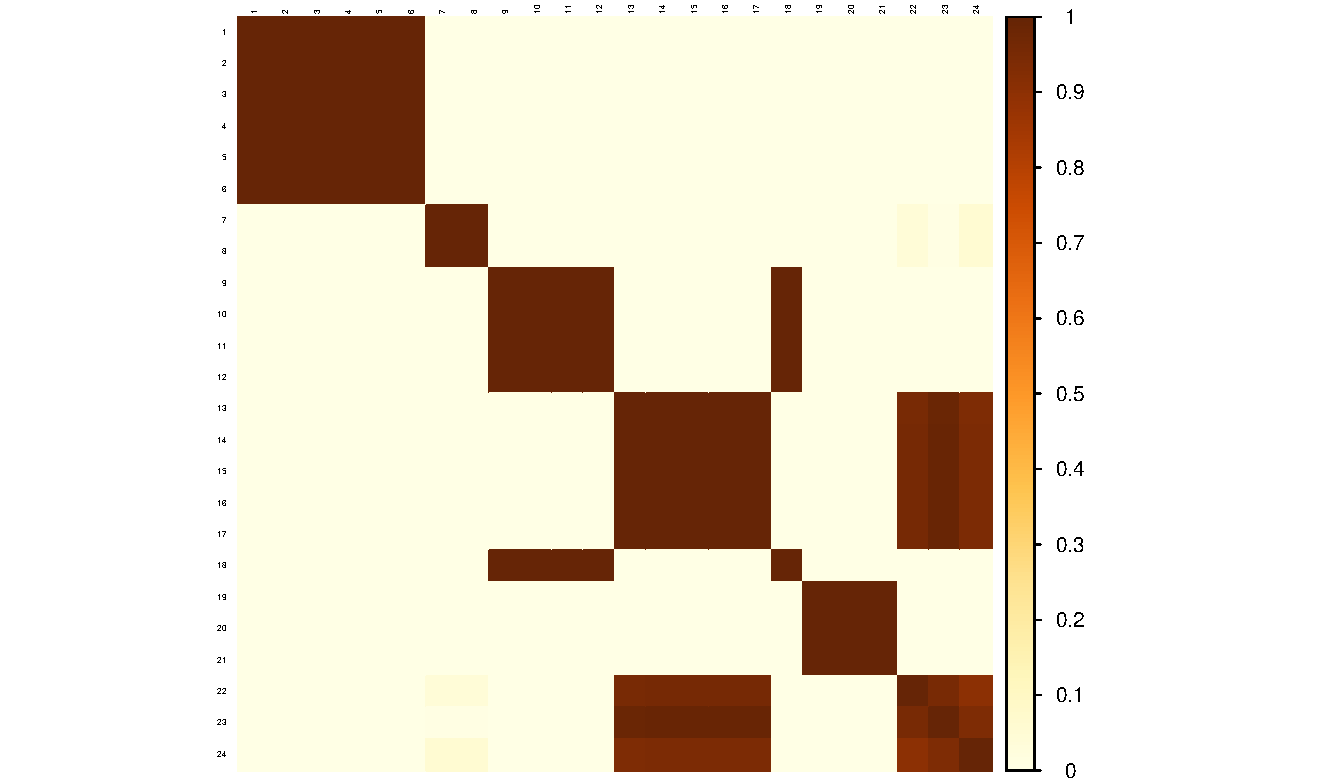
\includegraphics[width=\textwidth]{Kap3/chlrm_vi_A_fin.pdf}
        \caption*{(b) Final adjacency}
    \end{minipage}
    \caption{Adjacency matrices: co–assignment probabilities between groups under VI, farms dataset.}
    \label{fig:chlrm_vi_A_compare}
\end{figure}

\begin{figure}[H]
    \centering
    \begin{minipage}{0.5\textwidth}
        \centering
        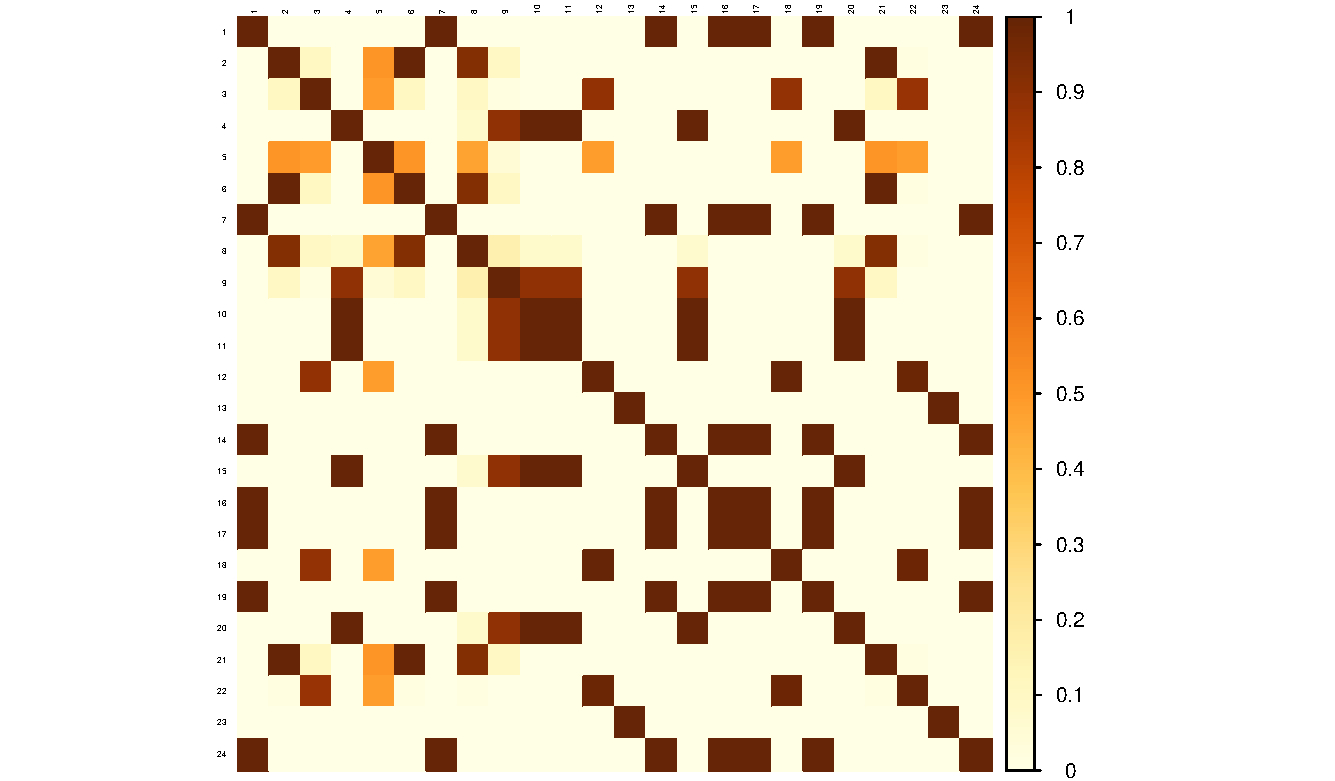
\includegraphics[width=\textwidth]{Kap3/chlrm_svi_A_init.pdf}
        \caption*{(a) Initial adjacency}
    \end{minipage}\hfill
    \begin{minipage}{0.5\textwidth}
        \centering
        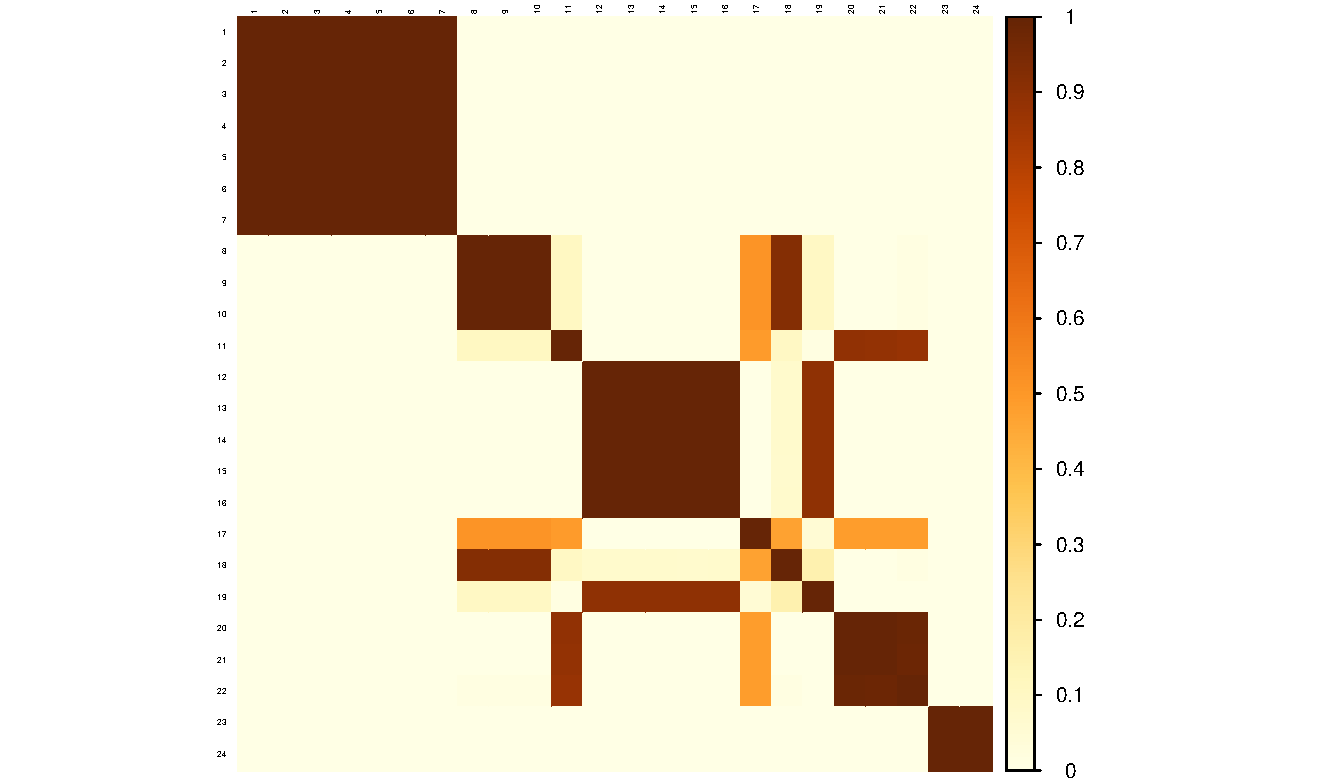
\includegraphics[width=\textwidth]{Kap3/chlrm_svi_A_fin.pdf}
        \caption*{(b) Final adjacency}
    \end{minipage}
    \caption{Adjacency matrices: co–assignment probabilities between groups under SVI, farms dataset.}
    \label{fig:chlrm_svi_A_compare}
\end{figure}

The adjacency matrices in Figures \ref{fig:chlrm_mcmc_A_compare}, \ref{fig:chlrm_vi_A_compare}, and \ref{fig:chlrm_svi_A_compare} provide a qualitative assessment of co–assignment probabilities. MCMC gradually transitions from diffuse initial states to sharper block structures, reflecting its ability to capture fine–grained posterior co–clustering. VI converges more quickly to rigid partitions, but with reduced representation of uncertainty. SVI strikes a balance: its final adjacency matrices show clear cluster delineation achieved in shorter time, though with additional stochastic variability introduced by mini–batch updates. 

\vspace{0.5cm}

In summary, the farms dataset highlights the core trade–offs of MCMC, VI, and SVI in clustered hierarchical regression. MCMC provides the most faithful posterior inference, as reflected in lower information criteria and richer adjacency structures, but at prohibitive computational cost. VI offers speed and stable convergence, producing sharp predictive fits at the expense of underestimating posterior variance. SVI emerges as a middle ground: it scales efficiently, delivers predictive accuracy close to VI, and produces adjacency structures that capture cluster patterns more robustly than VI alone, but it inherits stochastic noise and some bias in posterior uncertainty. Thus, while MCMC remains the gold standard in terms of posterior fidelity, VI and SVI provide practical alternatives when runtime and scalability are critical, particularly in datasets with weak cluster separation.
